\documentclass[]{report}
\usepackage{lmodern}
\usepackage{amssymb,amsmath}
\usepackage{ifxetex,ifluatex}
\usepackage{fixltx2e} % provides \textsubscript
\ifnum 0\ifxetex 1\fi\ifluatex 1\fi=0 % if pdftex
  \usepackage[T1]{fontenc}
  \usepackage[utf8]{inputenc}
\else % if luatex or xelatex
  \ifxetex
    \usepackage{mathspec}
  \else
    \usepackage{fontspec}
  \fi
  \defaultfontfeatures{Ligatures=TeX,Scale=MatchLowercase}
\fi
% use upquote if available, for straight quotes in verbatim environments
\IfFileExists{upquote.sty}{\usepackage{upquote}}{}
% use microtype if available
\IfFileExists{microtype.sty}{%
\usepackage{microtype}
\UseMicrotypeSet[protrusion]{basicmath} % disable protrusion for tt fonts
}{}
\usepackage[margin=1in]{geometry}
\usepackage{hyperref}
\hypersetup{unicode=true,
            pdftitle={MyBook},
            pdfauthor={Corinna Trierweiler and Philipp Gaulke},
            pdfborder={0 0 0},
            breaklinks=true}
\urlstyle{same}  % don't use monospace font for urls
\usepackage{natbib}
\bibliographystyle{plainnat}
\usepackage{color}
\usepackage{fancyvrb}
\newcommand{\VerbBar}{|}
\newcommand{\VERB}{\Verb[commandchars=\\\{\}]}
\DefineVerbatimEnvironment{Highlighting}{Verbatim}{commandchars=\\\{\}}
% Add ',fontsize=\small' for more characters per line
\usepackage{framed}
\definecolor{shadecolor}{RGB}{248,248,248}
\newenvironment{Shaded}{\begin{snugshade}}{\end{snugshade}}
\newcommand{\KeywordTok}[1]{\textcolor[rgb]{0.13,0.29,0.53}{\textbf{#1}}}
\newcommand{\DataTypeTok}[1]{\textcolor[rgb]{0.13,0.29,0.53}{#1}}
\newcommand{\DecValTok}[1]{\textcolor[rgb]{0.00,0.00,0.81}{#1}}
\newcommand{\BaseNTok}[1]{\textcolor[rgb]{0.00,0.00,0.81}{#1}}
\newcommand{\FloatTok}[1]{\textcolor[rgb]{0.00,0.00,0.81}{#1}}
\newcommand{\ConstantTok}[1]{\textcolor[rgb]{0.00,0.00,0.00}{#1}}
\newcommand{\CharTok}[1]{\textcolor[rgb]{0.31,0.60,0.02}{#1}}
\newcommand{\SpecialCharTok}[1]{\textcolor[rgb]{0.00,0.00,0.00}{#1}}
\newcommand{\StringTok}[1]{\textcolor[rgb]{0.31,0.60,0.02}{#1}}
\newcommand{\VerbatimStringTok}[1]{\textcolor[rgb]{0.31,0.60,0.02}{#1}}
\newcommand{\SpecialStringTok}[1]{\textcolor[rgb]{0.31,0.60,0.02}{#1}}
\newcommand{\ImportTok}[1]{#1}
\newcommand{\CommentTok}[1]{\textcolor[rgb]{0.56,0.35,0.01}{\textit{#1}}}
\newcommand{\DocumentationTok}[1]{\textcolor[rgb]{0.56,0.35,0.01}{\textbf{\textit{#1}}}}
\newcommand{\AnnotationTok}[1]{\textcolor[rgb]{0.56,0.35,0.01}{\textbf{\textit{#1}}}}
\newcommand{\CommentVarTok}[1]{\textcolor[rgb]{0.56,0.35,0.01}{\textbf{\textit{#1}}}}
\newcommand{\OtherTok}[1]{\textcolor[rgb]{0.56,0.35,0.01}{#1}}
\newcommand{\FunctionTok}[1]{\textcolor[rgb]{0.00,0.00,0.00}{#1}}
\newcommand{\VariableTok}[1]{\textcolor[rgb]{0.00,0.00,0.00}{#1}}
\newcommand{\ControlFlowTok}[1]{\textcolor[rgb]{0.13,0.29,0.53}{\textbf{#1}}}
\newcommand{\OperatorTok}[1]{\textcolor[rgb]{0.81,0.36,0.00}{\textbf{#1}}}
\newcommand{\BuiltInTok}[1]{#1}
\newcommand{\ExtensionTok}[1]{#1}
\newcommand{\PreprocessorTok}[1]{\textcolor[rgb]{0.56,0.35,0.01}{\textit{#1}}}
\newcommand{\AttributeTok}[1]{\textcolor[rgb]{0.77,0.63,0.00}{#1}}
\newcommand{\RegionMarkerTok}[1]{#1}
\newcommand{\InformationTok}[1]{\textcolor[rgb]{0.56,0.35,0.01}{\textbf{\textit{#1}}}}
\newcommand{\WarningTok}[1]{\textcolor[rgb]{0.56,0.35,0.01}{\textbf{\textit{#1}}}}
\newcommand{\AlertTok}[1]{\textcolor[rgb]{0.94,0.16,0.16}{#1}}
\newcommand{\ErrorTok}[1]{\textcolor[rgb]{0.64,0.00,0.00}{\textbf{#1}}}
\newcommand{\NormalTok}[1]{#1}
\usepackage{longtable,booktabs}
\usepackage{graphicx,grffile}
\makeatletter
\def\maxwidth{\ifdim\Gin@nat@width>\linewidth\linewidth\else\Gin@nat@width\fi}
\def\maxheight{\ifdim\Gin@nat@height>\textheight\textheight\else\Gin@nat@height\fi}
\makeatother
% Scale images if necessary, so that they will not overflow the page
% margins by default, and it is still possible to overwrite the defaults
% using explicit options in \includegraphics[width, height, ...]{}
\setkeys{Gin}{width=\maxwidth,height=\maxheight,keepaspectratio}
\IfFileExists{parskip.sty}{%
\usepackage{parskip}
}{% else
\setlength{\parindent}{0pt}
\setlength{\parskip}{6pt plus 2pt minus 1pt}
}
\setlength{\emergencystretch}{3em}  % prevent overfull lines
\providecommand{\tightlist}{%
  \setlength{\itemsep}{0pt}\setlength{\parskip}{0pt}}
\setcounter{secnumdepth}{5}
% Redefines (sub)paragraphs to behave more like sections
\ifx\paragraph\undefined\else
\let\oldparagraph\paragraph
\renewcommand{\paragraph}[1]{\oldparagraph{#1}\mbox{}}
\fi
\ifx\subparagraph\undefined\else
\let\oldsubparagraph\subparagraph
\renewcommand{\subparagraph}[1]{\oldsubparagraph{#1}\mbox{}}
\fi

%%% Use protect on footnotes to avoid problems with footnotes in titles
\let\rmarkdownfootnote\footnote%
\def\footnote{\protect\rmarkdownfootnote}

%%% Change title format to be more compact
\usepackage{titling}

% Create subtitle command for use in maketitle
\providecommand{\subtitle}[1]{
  \posttitle{
    \begin{center}\large#1\end{center}
    }
}

\setlength{\droptitle}{-2em}

  \title{MyBook}
    \pretitle{\vspace{\droptitle}\centering\huge}
  \posttitle{\par}
    \author{Corinna Trierweiler and Philipp Gaulke}
    \preauthor{\centering\large\emph}
  \postauthor{\par}
      \predate{\centering\large\emph}
  \postdate{\par}
    \date{2019-07-26}

\usepackage{booktabs}
\usepackage{amsthm}
\makeatletter
\def\thm@space@setup{%
  \thm@preskip=8pt plus 2pt minus 4pt
  \thm@postskip=\thm@preskip
}
\makeatother

\begin{document}
\maketitle

{
\setcounter{tocdepth}{1}
\tableofcontents
}
\chapter*{Preface}\label{preface}
\addcontentsline{toc}{chapter}{Preface}

This book has been produced for and based on the Data Science class of
Hochschule Fresenius in Cologne, Germany. In context of the task, the
book includes basic R skills, statistical methods for data science and a
solution for the exercise given at the end of the semester.

\chapter*{Introduction}\label{introduction}
\addcontentsline{toc}{chapter}{Introduction}

This book is created in order to provide programming beginners a clear
and understandable overview of how to use R for statistical
investigations. This includes the explanation for the set up and an
introduction to the basic skills for R, as well as an overview of major
statistical methods for data science.

\begin{itemize}
\tightlist
\item
  What is R? -
\end{itemize}

R is a programming language and free software environment for
statistical computing created by the R Foundation for Statistical
Computing. It is a common tool to create statistical software that can
be used to analyze and interprete data sets. Apart from the ground
infrastructure and function, R can be individualized easy and quickly by
downloading additional tools and packages which are free avalaibale.
These packages may include further function for calculation, data sets
or even own programming features.

\begin{itemize}
\tightlist
\item
  How do we approach it? -
\end{itemize}

Learning programming is broadly declared as a herculean task. Firstly,
this is simply not true especially when you consider that most of us
learn a second real language in the age of 10, which is by far more
difficult. Secondly, learning success is like everywhere else depending
on how you approach it. Opening in the first step some R file and apply
random statistical methods on a 7 terrabyte file will most probably not
lead to a result that makes any sense, especially when you are not too
familiar with statistics. However, in the following we will make one
step after the other, so that any of you will be able to follow and
understand the next step. This will include at first the software
set-up, which is quite easy but highly important for further steps.
After that, we will introduce you the structure of R and the basic
skills. Having you then on a ``I now somehow know how to import and
calculate things''-level we will go over to the statistical part. Before
you now go on and start with your R career, answer yourself some
questions:

\begin{itemize}
\item
  Are you able to read, write and calculate?
\item
  Have you ever worked on a computer in your life (surfing, writing a
  text or dowload something?)
\item
  Are you actually interested in how to understand and analyze data?
\end{itemize}

If there is any ``No'' here, then think about it once again. As already
said, this is not a herculean task but of course it will need some
effort and time to get into R. If it is ``yes, yes, and yes'' then
great! Let's get started, you will probably be able to write ``Basic R
skills'' into your CV, before you even think about it.

\part{Explaining R}\label{part-explaining-r}

\chapter{Setup}\label{setup}

You will need the following software:

The R software itself, RStudio (so to say, the environment where you
will work in) and a Latex distribution for creating output files such as
pdf files with R graphics.

R Software - \url{https://cran.uni-muenster.de/}

FreeVersion of RStudio -
\url{https://www.rstudio.com/products/rstudio/download/\#download}

Latex distribution - for example:
\url{https://www.latex-project.org/get/} (depending on your software)

\section{Start Your Project}\label{start-your-project}

In order to share your work, GitHub is a tool of major importance. In
the following, we will explain to you how to set this up. It is totally
up to you whether to install it now or later. Please just consider, that
you should install it before you start your project. Otherwise you will
face a quite complicated process and limited possibilities to fully
enjoy all collaborational features that GitHub provides.

The software you need for this is Git Distribution.

Git distribution - \url{https://git-scm.com/downloads}

In parallel of installing the Git distribution, go to
\url{https://github.com} and create an account.

In a first step, you should activate Git in RStudio. Therefore choose:
`Tools' \textgreater{} `Global Options' \textgreater{} `Git/SVN' and
click on the button to enable the version control interface.
Additionally, you should generate a SHH RSA key which will be needed in
a later stage when setting up your repository on GitHub.

Now you can create your project. Click on `File' \textgreater{} `New
Project' \textgreater{} `Existing directory' and choose where you want
to place your project on your computer. Be aware, that you really know
where you place it as you will need the directory in a later stage.

Now it is time to prepare for the marriage of your GitHub account and
your project. Go to GitHub and create a new repository and name it
exactly the same way as you named your R project. The naming has to be
identical. Next, got to your settings in GitHub and choose `SHH and GPG
Keys' and click on `New SHH key'. Go back to RStudio and copy the SHH
key that has been created in the first step, then paste it into your
GitHub account.

Now everything is set up to create the connection. In order to do so, go
in RStudio to `Tools' \textgreater{} `Project Options' \textgreater{}
`Git/SVN'. Select `Git' in the Version control system field. After that,
go again to `Tools' \textgreater{} `Terminal' \textgreater{} `New
Terminal'. Now next to the console a terminal should appear.

As you may already read when you finished your the creation of your
repository, here you should type in the following commands:

\begin{Shaded}
\begin{Highlighting}[]
\NormalTok{git init}


\NormalTok{git remote add origin https}\OperatorTok{:}\ErrorTok{//}\NormalTok{github.com}\OperatorTok{/}\NormalTok{YOURNAME}\OperatorTok{/}\NormalTok{YOURREPOSITORY.git}
\NormalTok{git push }\OperatorTok{-}\NormalTok{u origin master}
\end{Highlighting}
\end{Shaded}

Obvisously you should adopt the origin link with your own names.

Now restart RStudio and enjoy that you just completed to connect your
project with GitHub. In the upper right corner of RStudio you should now
see a Git button (right next to environment/history/connections). To put
your files on GitHub, you can now easily commit and then push all files
you want to share.

\section{Work Collaboratively}\label{work-collaboratively}

If you are interested to work simoultanesly with another person on one
project, you can create a team in GitHub. However, this is not done by a
few clicks.

At first, you have to decide who the owner of the project should be. The
role will not have too much influence later on, but it defines the set
up for each participant.

The project owner needs to create an organization on Github. Within this
organization a new repository should be created, which again should have
exactly the same name as the project in R Studio. Herefore, you can
follow the steps described above. If you have done that, you should
create a team in the organization and add the further participants to
the team. Be aware that you should assign the repository to these
members and provide the members with respective rights.

As the team member who should have received an email at this point.
After you confirmed the participation, go onto the repository and click
on the button `Clone or download'. Look for the https adress, copy it
and go now into a simple RStudio session (not a project). Open a new
Terminal and type in cd with the path where you want to save the
project. Now typ `git clone' and paste the the copied link from GitHub.

\begin{Shaded}
\begin{Highlighting}[]
\NormalTok{cd Dropbox}\OperatorTok{/}\NormalTok{Master}\OperatorTok{/}\NormalTok{2Sem}
\NormalTok{git clone https}\OperatorTok{:}\ErrorTok{//}\NormalTok{github.com}\OperatorTok{/}\NormalTok{ORGANIZATION}\OperatorTok{/}\NormalTok{repo.git }
\end{Highlighting}
\end{Shaded}

Now you should finally be able to push and pull the all files and start
your collaborative R project.

\chapter{Creating Files in R}\label{creating-files-in-r}

For working in R we use R Markdown documents. Click on `File'
\textgreater{} `New File' and then create a new R Markdown file. R
Markdown files include simple formatting syntax for authoring HTML, PDF
and Microsoft Word documents. If you look for any specific information
about R Markdown which is not included in this book, check this link
\url{http://rmarkdown.rstudio.com}.

Basically, there are two ways to add something to an R Markdown file.

\begin{itemize}
\tightlist
\item
  Written text, in which you can include some inline-code by starting
  with a backstick plus r and ending with a backstick e.g.~6. However
  this kind of code integration will be used less often in this book.
\item
  Chunks, seperate grey fields that are used to integrate code. You can
  create a chunk by entering three backsticks plus \{r\} and end it with
  again three backticks
\end{itemize}

Below a short example for a chunk

\begin{Shaded}
\begin{Highlighting}[]
\DecValTok{2}\OperatorTok{*}\DecValTok{3}
\end{Highlighting}
\end{Shaded}

\begin{verbatim}
## [1] 6
\end{verbatim}

In order to process the operation that you entered, you have to click on
the green arrow in the right corner. This is what we call to run a
chunk. While working through this book, you will create many chunks with
different operations. This includes not only mathematical operations,
but also the creation of graphs. There are various ways how to write
code in a chunk, we will provide you in the following chapters with more
insights, so that you will be able chose the most efficient and fastest
ways for each purpose.

In the following, both ways of adding something to a R Markdown file
will be illustrated in detail.

\section{Designing written text}\label{designing-written-text}

General advises of how to edit written text can you find on the
following website:
\url{https://www.rstudio.com/wp-content/uploads/2015/02/rmarkdown-cheatsheet.pdf}

This cheatsheet contains all inline-formatting options that you can use
in base R. It also shows you how to understand the use of block level
elements. By using a hashtag, you can create headlines. The logic is
that:

One \# - main-headline Two \# - sub-headline Three \# - sub-headline of
degree 2

It is important to know that you can only use on main-headline per R
markdown file. In order to include more main-headlines you should
another R markdown file in your project. For example, in case that you
create a book it is recommendable to create one R markdown file per
chapter. That is not only more attractive because of the usability of
main-headline, but it also provides a better overview of your work.

Of course, formatting is not limited to that. The actual output can be
edited in various ways by using YAML. You find your YAML-header in each
of your R markdown files. However, if you want to adopt your files
generally rather than specific for each R markdown file you can use the
output.yml file. As soon as you create a project, you will find a file
in your project that is called output.yml. Settings that you include
here will work as a standard for your project, so that you do not need
to adopt each R markdown file.

Considering that you probably want to produce a book, respectively
create output in form of a PDF, HTML, or other kind of file, it will be
necessary to include some information in the header.

For example, if you want to build a PDF file, you have to include:

\begin{verbatim}
bookdown::pdf_book:
  includes:
    in_header: preamble.tex
\end{verbatim}

However, for further information on how to produce output, please check
Chapter 3 - (\citet{ref/Creation} of Output)

HIER NOCH EINE INFORMATION ZU DEN GESTALTUNGSMÖGLICHKEITEN BEI YAML

\section{Coding in chunks}\label{coding-in-chunks}

Actually, this is the main topic of this book. The explanation of coding
in R chunks will not be limited to this chapter, but at this point it is
helpful to get an overview of how chunks work and what you can do with
them.

The sample chunk in the beginning of this chapter, already revealed the
general functionality. Nevertheless, there some general notes to make.

\subsection{Chunk options}\label{chunk-options}

At first, different options can be set for a chunk, for example wheter
to evaluate the code chunk, to stop processing when an error occurs, or
to dispay the source code in your output file and a lot more. This can
be done by editing the content of the brackets.

If you add eval=TRUE/FALSE, then the whole chunk will be evaluated
respectively not evaluated.

\begin{Shaded}
\begin{Highlighting}[]
\DecValTok{42}\OperatorTok{+}\DecValTok{17}
\end{Highlighting}
\end{Shaded}

\begin{verbatim}
## [1] 59
\end{verbatim}

\begin{Shaded}
\begin{Highlighting}[]
\DecValTok{82}\OperatorTok{-}\DecValTok{2}
\end{Highlighting}
\end{Shaded}

\begin{verbatim}
## [1] 80
\end{verbatim}

\begin{Shaded}
\begin{Highlighting}[]
\DecValTok{42}\OperatorTok{+}\DecValTok{17}
\DecValTok{82}\OperatorTok{-}\DecValTok{2}
\end{Highlighting}
\end{Shaded}

If you add error=TRUE/FALSE, then the run-process will be stopped,
respecitively not stopped, if an error occures.

\begin{Shaded}
\begin{Highlighting}[]
\DecValTok{100}\OperatorTok{*}\NormalTok{apples}
\DecValTok{9}\OperatorTok{*}\DecValTok{3}
\end{Highlighting}
\end{Shaded}

\begin{Shaded}
\begin{Highlighting}[]
\DecValTok{100}\OperatorTok{*}\NormalTok{apples}
\DecValTok{9}\OperatorTok{*}\DecValTok{3}
\end{Highlighting}
\end{Shaded}

If you add echo=TRUE/FALSE, then the source code will be displayed
respecitively not displayed in the output file.

\begin{Shaded}
\begin{Highlighting}[]
\DecValTok{10}\OperatorTok{+}\DecValTok{27}
\end{Highlighting}
\end{Shaded}

\begin{verbatim}
## [1] 37
\end{verbatim}

\begin{Shaded}
\begin{Highlighting}[]
\DecValTok{8}\OperatorTok{+}\DecValTok{6}
\end{Highlighting}
\end{Shaded}

\begin{verbatim}
## [1] 14
\end{verbatim}

\begin{verbatim}
## [1] 37
\end{verbatim}

\begin{verbatim}
## [1] 14
\end{verbatim}

For a detailed explanation for most of all options, please see here
\url{https://yihui.name/knitr/options/}.

Looking into what you can add into the chunk, you have to be aware that
any small mistake will mess up the whole chunk. Especially, for larger
and more complex chunks this is a challenge. Therefore, it might be a
good idea to make comments for later understanding. Comments can be made
by using a hashtag when starting a new line in a chunk. Here an example:

\begin{Shaded}
\begin{Highlighting}[]
\DecValTok{10}\OperatorTok{*}\DecValTok{750000}\OperatorTok{/}\DecValTok{17}
\end{Highlighting}
\end{Shaded}

\begin{verbatim}
## [1] 441176.5
\end{verbatim}

\begin{Shaded}
\begin{Highlighting}[]
\CommentTok{#Just a random calculation}
\end{Highlighting}
\end{Shaded}

\subsection{Chunk Functions}\label{chunk-functions}

As a basic, we can use the chunk as a \emph{calculator}.

We can build up easier calculations as well as more difficult
calculations, as far as our keyboard allows us.

\begin{Shaded}
\begin{Highlighting}[]
\DecValTok{8}\OperatorTok{*}\DecValTok{4}\OperatorTok{+}\DecValTok{12}
\end{Highlighting}
\end{Shaded}

\begin{verbatim}
## [1] 44
\end{verbatim}

\begin{Shaded}
\begin{Highlighting}[]
\DecValTok{37}\OperatorTok{*}\DecValTok{4235}\OperatorTok{+}\NormalTok{(}\DecValTok{19}\OperatorTok{*}\DecValTok{245}\NormalTok{)}\OperatorTok{/}\DecValTok{422}\OperatorTok{+}\DecValTok{3}\OperatorTok{-}\DecValTok{10}
\end{Highlighting}
\end{Shaded}

\begin{verbatim}
## [1] 156699
\end{verbatim}

\begin{Shaded}
\begin{Highlighting}[]
\KeywordTok{sin}\NormalTok{(}\DecValTok{40}\OperatorTok{*}\DecValTok{9}\NormalTok{)}\OperatorTok{+}\KeywordTok{log}\NormalTok{(}\DecValTok{120}\NormalTok{)}
\end{Highlighting}
\end{Shaded}

\begin{verbatim}
## [1] 5.746407
\end{verbatim}

Moreover, R provides built-in functions that you can easily use to
exercise special operations. In the following example, a sequence will
be created by using the function - seq -

\begin{Shaded}
\begin{Highlighting}[]
\KeywordTok{seq}\NormalTok{(}\DecValTok{1}\NormalTok{,}\DecValTok{5}\NormalTok{)}
\end{Highlighting}
\end{Shaded}

\begin{verbatim}
## [1] 1 2 3 4 5
\end{verbatim}

\begin{Shaded}
\begin{Highlighting}[]
\KeywordTok{seq}\NormalTok{(}\DecValTok{1}\NormalTok{,}\DecValTok{10}\NormalTok{,}\DataTypeTok{length.out =} \DecValTok{3}\NormalTok{)}
\end{Highlighting}
\end{Shaded}

\begin{verbatim}
## [1]  1.0  5.5 10.0
\end{verbatim}

More built-in functions can be found under the following link:
\url{https://www.statmethods.net/management/functions.html}

Another function that is included in chunks is to \emph{name
operations}. Naming advantages can be beneficial if you want to use the
operational multiple times in your chunk.

\begin{Shaded}
\begin{Highlighting}[]
\NormalTok{a <-}\DecValTok{905}\OperatorTok{/}\DecValTok{12}\OperatorTok{*}\DecValTok{5}

\KeywordTok{sin}\NormalTok{(a)}\OperatorTok{+}\KeywordTok{sin}\NormalTok{(a}\OperatorTok{^}\DecValTok{2}\NormalTok{)}\OperatorTok{+}\KeywordTok{sin}\NormalTok{(a}\OperatorTok{^}\DecValTok{3}\NormalTok{)}
\end{Highlighting}
\end{Shaded}

\begin{verbatim}
## [1] 0.8484134
\end{verbatim}

\chapter{Creation of output}\label{creation-of-output}

By selecting Knit you can create a file out of your .rmd's. R Studio
supports various formats which you can set in the header of any .rmd
file.

\begin{Shaded}
\begin{Highlighting}[]
\NormalTok{output}\OperatorTok{:}\StringTok{ }\NormalTok{html_document}
\end{Highlighting}
\end{Shaded}

Otherwise you can also select a format in the dropdown menu oft the
Knit-button.

Of course, there are various ways of formatting your output. Herefore,
you have to use the fields below your output format in the header. To
know which options you can choose for every output format, just check
the respective help page. To open the help page, you have to type in
?rmarkdown::(here output format) into the console.

Another option you have, is to build a book. In case you want to compile
all your rmd.file to one book, you can call the render function in
bookdown. In order to this, you have to download the bookdown package.
This is easily done, by clicking on \emph{Tools}, then \emph{Install
packages} and search for bookdown. There is more than only one way to
download packages, also chunks provide this option by searching for the
packages like this:

\begin{Shaded}
\begin{Highlighting}[]
\KeywordTok{install.packages}\NormalTok{(}\StringTok{"bookdown"}\NormalTok{)}
\end{Highlighting}
\end{Shaded}

To now prepare for building a book, please go into the .yml file of your
project and set the options up accordingly. For example to create a .pdf
book, type in this:

\begin{Shaded}
\begin{Highlighting}[]
\NormalTok{bookdown}\OperatorTok{::}\NormalTok{pdf_book}\OperatorTok{:}
\end{Highlighting}
\end{Shaded}

This should then be further set up, for options you can again use the
console:

\begin{Shaded}
\begin{Highlighting}[]
\NormalTok{?bookdown}\OperatorTok{::}\NormalTok{pdf}\OperatorTok{:}\NormalTok{book}
\end{Highlighting}
\end{Shaded}

\chapter{Basic R Skills}\label{basic-r-skills}

Now we dive a little bit deeper into R and go trough the basics of how
to handle data. For this, it is necessary to get an understanding of the
most important data structures that do exist, what kind of data they may
include and in what kind of format they are. Furthermore, we will
introduce you some major rules which should be considered while handling
data in R as well as how to import data and what packages might be
useful in order to handle data effective and efficiently. Before closing
this chapter, also a short overview on how to visualize data is given.

After gathering all the informations and knowledge, it will be possible
for you to work with statistics in R, which will be the topic of the
second part of this book.

\section{Data stuctures}\label{data-stuctures}

In general there are four types of data structures: atomic vectors,
lists, matrix and arrays, and data frames.

The most common type of data structure are \emph{atomic vectors}.
Vectors can be described by three attributes:

\begin{enumerate}
\def\labelenumi{\arabic{enumi}.}
\tightlist
\item
  the type \texttt{typeof()}
\end{enumerate}

Vectors can be either numeric, logical, or character.

\begin{Shaded}
\begin{Highlighting}[]
\NormalTok{numeric_vector <-}\StringTok{ }\KeywordTok{c}\NormalTok{(}\DecValTok{1}\NormalTok{,}\DecValTok{2}\NormalTok{,}\DecValTok{3}\NormalTok{,}\DecValTok{4}\NormalTok{,}\DecValTok{5}\NormalTok{) }\CommentTok{# numeric vector}
\NormalTok{logical_vector <-}\StringTok{ }\KeywordTok{c}\NormalTok{(}\OtherTok{TRUE}\NormalTok{,}\OtherTok{TRUE}\NormalTok{,}\OtherTok{TRUE}\NormalTok{,}\OtherTok{FALSE}\NormalTok{) }\CommentTok{# logical vector}
\NormalTok{character_vector <-}\StringTok{ }\KeywordTok{c}\NormalTok{(}\StringTok{"first"}\NormalTok{, }\StringTok{"apple"}\NormalTok{, }\StringTok{"child"}\NormalTok{, }\StringTok{"word"}\NormalTok{) }\CommentTok{# character vector}
\end{Highlighting}
\end{Shaded}

Further, you can also create integer and mixed vectors

\begin{Shaded}
\begin{Highlighting}[]
\NormalTok{integer_vector <-}\StringTok{ }\KeywordTok{c}\NormalTok{(10L, 4L, 7L) }\CommentTok{# integer vector}
\NormalTok{mixed_vector <-}\StringTok{ }\KeywordTok{c}\NormalTok{(}\DecValTok{2}\NormalTok{, }\StringTok{"mixed"}\NormalTok{) }\CommentTok{# mixed vector}
\end{Highlighting}
\end{Shaded}

When you create a mixed vector and you do not determine which type of
vector you create, than R decides on itself. The logic is: logical
\textless{} numeric \textless{} character.

Numeric vectors can be also created by only using `x:y' if you want to
include all numbers from x to y.

\begin{Shaded}
\begin{Highlighting}[]
\NormalTok{another_numeric <-}\StringTok{ }\DecValTok{1}\OperatorTok{:}\DecValTok{5}
\end{Highlighting}
\end{Shaded}

\begin{enumerate}
\def\labelenumi{\arabic{enumi}.}
\setcounter{enumi}{1}
\tightlist
\item
  the length \texttt{length()}
\end{enumerate}

The length basically describes the size of the vector. If you want to
check the length of a vector, you have to use \texttt{length()}.

\begin{Shaded}
\begin{Highlighting}[]
\NormalTok{whatisthelength <-}\StringTok{ }\KeywordTok{c}\NormalTok{(}\DecValTok{1}\NormalTok{,}\DecValTok{4}\NormalTok{,}\DecValTok{2}\NormalTok{,}\DecValTok{1}\NormalTok{,}\DecValTok{16}\NormalTok{,}\DecValTok{124}\NormalTok{,}\DecValTok{54}\NormalTok{,}\DecValTok{6}\NormalTok{,}\DecValTok{7}\NormalTok{)}

\KeywordTok{length}\NormalTok{(whatisthelength)}
\end{Highlighting}
\end{Shaded}

\begin{verbatim}
## [1] 9
\end{verbatim}

\begin{enumerate}
\def\labelenumi{\arabic{enumi}.}
\setcounter{enumi}{2}
\tightlist
\item
  the attributes \texttt{attributes()}
\end{enumerate}

Attributes define the nature of a specific vector and are relevant for
what kind of function can be applied. The three major attributes are:

\begin{itemize}
\tightlist
\item
  the names, \texttt{names()},
\item
  the dimensions, \texttt{dim()},
\item
  the class, \texttt{class}.
\end{itemize}

However, you can also check attributes in the summary of the vector.
Therefore, you have to use \texttt{summary()}, which is (as most all
other attributes) also applicable on other data structures.

\begin{Shaded}
\begin{Highlighting}[]
\NormalTok{atry <-}\StringTok{ }\KeywordTok{c}\NormalTok{(}\DecValTok{1}\OperatorTok{:}\DecValTok{15}\NormalTok{)}
\KeywordTok{summary}\NormalTok{(atry)}
\end{Highlighting}
\end{Shaded}

\begin{verbatim}
##    Min. 1st Qu.  Median    Mean 3rd Qu.    Max. 
##     1.0     4.5     8.0     8.0    11.5    15.0
\end{verbatim}

\begin{Shaded}
\begin{Highlighting}[]
\NormalTok{anothertry <-}\StringTok{ }\KeywordTok{c}\NormalTok{(T,F,T,F)  }
\KeywordTok{summary}\NormalTok{(anothertry)}
\end{Highlighting}
\end{Shaded}

\begin{verbatim}
##    Mode   FALSE    TRUE 
## logical       2       2
\end{verbatim}

Another type of data structure are \emph{lists}. A list can include a
number of objects, but also another list. Therefore, it is useful in
order to gather data into one structure.

\begin{Shaded}
\begin{Highlighting}[]
\NormalTok{alist <-}\StringTok{ }\KeywordTok{list}\NormalTok{(}\DataTypeTok{numbers=}\KeywordTok{c}\NormalTok{(}\DecValTok{1}\OperatorTok{:}\DecValTok{10}\NormalTok{),}
      \DataTypeTok{fruits=}\KeywordTok{c}\NormalTok{(}\StringTok{"Banana"}\NormalTok{, }\StringTok{"Peach"}\NormalTok{),}
      \DataTypeTok{values=}\KeywordTok{c}\NormalTok{(T,T,F,T,F))}
\NormalTok{alist}
\end{Highlighting}
\end{Shaded}

\begin{verbatim}
## $numbers
##  [1]  1  2  3  4  5  6  7  8  9 10
## 
## $fruits
## [1] "Banana" "Peach" 
## 
## $values
## [1]  TRUE  TRUE FALSE  TRUE FALSE
\end{verbatim}

If you want to illustrate a \emph{matrix} than you can also use R for
this. Therefore, you have to consider that all columns have the same
mode and the same length. In general the formel to use is:

\begin{Shaded}
\begin{Highlighting}[]
\NormalTok{amatrix <-}\StringTok{ }\KeywordTok{matrix}\NormalTok{(}\KeywordTok{c}\NormalTok{(}\DecValTok{1}\OperatorTok{:}\DecValTok{12}\NormalTok{), }\DataTypeTok{nrow=}\DecValTok{4}\NormalTok{, }\DataTypeTok{ncol=}\DecValTok{3}\NormalTok{) }
\NormalTok{amatrix}
\end{Highlighting}
\end{Shaded}

\begin{verbatim}
##      [,1] [,2] [,3]
## [1,]    1    5    9
## [2,]    2    6   10
## [3,]    3    7   11
## [4,]    4    8   12
\end{verbatim}

Another essential data structure are \emph{data frames}. Somehow the
data frame is similar to the matrix, but you can use different modes.
Apart from some build-in data sets that are provided in a data frame
layout, you can create a data frame by yourself by using the function
data.frame.

\begin{Shaded}
\begin{Highlighting}[]
\NormalTok{adf <-}\StringTok{ }\KeywordTok{data.frame}\NormalTok{(}\DataTypeTok{numbers=}\DecValTok{1}\OperatorTok{:}\DecValTok{4}\NormalTok{,}
                  \DataTypeTok{fruits=} \KeywordTok{c}\NormalTok{(}\StringTok{"banana"}\NormalTok{, }\StringTok{"peaches"}\NormalTok{, }\StringTok{"orange"}\NormalTok{, }\StringTok{"strawberry"}\NormalTok{),}
                  \DataTypeTok{value=} \KeywordTok{c}\NormalTok{(T,F,F,T))}
\NormalTok{adf}
\end{Highlighting}
\end{Shaded}

\begin{verbatim}
##   numbers     fruits value
## 1       1     banana  TRUE
## 2       2    peaches FALSE
## 3       3     orange FALSE
## 4       4 strawberry  TRUE
\end{verbatim}

By the way, the length of data frame is determined by the number of
columns you include. For our example, you can check the length like
this:

\begin{Shaded}
\begin{Highlighting}[]
\NormalTok{adf <-}\StringTok{ }\KeywordTok{data.frame}\NormalTok{(}\DataTypeTok{numbers=}\DecValTok{1}\OperatorTok{:}\DecValTok{4}\NormalTok{,}
                  \DataTypeTok{fruits=} \KeywordTok{c}\NormalTok{(}\StringTok{"banana"}\NormalTok{, }\StringTok{"peaches"}\NormalTok{, }\StringTok{"orange"}\NormalTok{, }\StringTok{"strawberry"}\NormalTok{),}
                  \DataTypeTok{value=} \KeywordTok{c}\NormalTok{(T,F,F,T))}
\KeywordTok{length}\NormalTok{(adf)}
\end{Highlighting}
\end{Shaded}

\begin{verbatim}
## [1] 3
\end{verbatim}

\section{Principles in R Chunks}\label{principles-in-r-chunks}

There are some major calculation principles that you have to consider
while working with R. For instance, these principles can be quite
helpful but being not aware of there existence might lead to errors that
are difficult to detect.

At first, we have to consider that \emph{element by element evaluation}
is active. In case that you want to somehow create a calculation with
two or more vectors, this principle is of major importance.

In case of two numeric vectors of the same length, the calculation will
be applied on each element in the same position.

\begin{Shaded}
\begin{Highlighting}[]
\NormalTok{store1revenue <-}\StringTok{ }\KeywordTok{c}\NormalTok{(}\DecValTok{10000}\NormalTok{,}\DecValTok{12000}\NormalTok{,}\DecValTok{18000}\NormalTok{,}\DecValTok{9000}\NormalTok{,}\DecValTok{11000}\NormalTok{)}
\NormalTok{store2revenue <-}\StringTok{ }\KeywordTok{c}\NormalTok{(}\DecValTok{25000}\NormalTok{,}\DecValTok{29000}\NormalTok{,}\DecValTok{21000}\NormalTok{,}\DecValTok{23000}\NormalTok{,}\DecValTok{24000}\NormalTok{)}

\KeywordTok{length}\NormalTok{(store1revenue) }\OperatorTok{==}\StringTok{ }\KeywordTok{length}\NormalTok{(store2revenue)}
\end{Highlighting}
\end{Shaded}

\begin{verbatim}
## [1] TRUE
\end{verbatim}

\begin{Shaded}
\begin{Highlighting}[]
\NormalTok{revenuesum <-}\StringTok{ }\NormalTok{store1revenue}\OperatorTok{+}\NormalTok{store2revenue}

\NormalTok{revenuesum}
\end{Highlighting}
\end{Shaded}

\begin{verbatim}
## [1] 35000 41000 39000 32000 35000
\end{verbatim}

Every element of the first vector is added to the element that is in the
same position in the second vector.

Now, if you violate the premise that the vectors used have the same
length, the second principle will be activated. \emph{Recycling} happens
and the objects included int he shortest vector will be repetivtively
used for the calculation.

\begin{Shaded}
\begin{Highlighting}[]
\NormalTok{performanceofa <-}\StringTok{ }\KeywordTok{c}\NormalTok{(}\DecValTok{34}\NormalTok{,}\DecValTok{39}\NormalTok{,}\DecValTok{51}\NormalTok{,}\DecValTok{45}\NormalTok{,}\DecValTok{28}\NormalTok{,}\DecValTok{37}\NormalTok{)}
\NormalTok{performanceofb <-}\StringTok{ }\KeywordTok{c}\NormalTok{(}\DecValTok{30}\NormalTok{,}\DecValTok{29}\NormalTok{,}\DecValTok{45}\NormalTok{,}\DecValTok{42}\NormalTok{)}
\NormalTok{performancesum <-}\StringTok{ }\NormalTok{performanceofa}\OperatorTok{+}\NormalTok{performanceofb}
\end{Highlighting}
\end{Shaded}

\begin{verbatim}
## Warning in performanceofa + performanceofb: Länge des längeren Objektes
##       ist kein Vielfaches der Länge des kürzeren Objektes
\end{verbatim}

\begin{Shaded}
\begin{Highlighting}[]
\NormalTok{performancesum}
\end{Highlighting}
\end{Shaded}

\begin{verbatim}
## [1] 64 68 96 87 58 66
\end{verbatim}

If recycing happens, you will receive an error message which is
apparently not an error message that is stopping any process, but making
you aware of the recycling.

Another important thing, which is less a principle but more a shortcut,
is the \emph{deletion of NA's}. Sometimes you want to take a vector for
a calculation that will take all values of that vector into account.
This might lead to difficulties, as missing values are often replaced
with \texttt{NA} in data sets. However, with using 'na.rm = T, R will
ignore the NA during the calculation.

\begin{Shaded}
\begin{Highlighting}[]
\NormalTok{horsepower <-}\StringTok{ }\KeywordTok{c}\NormalTok{(}\DecValTok{400}\NormalTok{,}\DecValTok{320}\NormalTok{,}\DecValTok{190}\NormalTok{,}\DecValTok{200}\NormalTok{,}\DecValTok{310}\NormalTok{,}\DecValTok{290}\NormalTok{,}\DecValTok{420}\NormalTok{,}\OtherTok{NA}\NormalTok{,}\DecValTok{230}\NormalTok{,}\DecValTok{220}\NormalTok{)}
\KeywordTok{mean}\NormalTok{(horsepower, }\DataTypeTok{na.rm =}\NormalTok{ T)}
\end{Highlighting}
\end{Shaded}

\begin{verbatim}
## [1] 286.6667
\end{verbatim}

\section{Subsetting}\label{subsetting}

Subsetting means to create a data set out of the existing data
structure. So to say, you copy particular items out of a data
collection.

There are three main operators which can be used to subset:

\begin{itemize}
\tightlist
\item
  \texttt{{[}{]}}
\item
  \texttt{{[}{[}{]}{]}}
\item
  \texttt{\$}
\end{itemize}

The first one, \texttt{{[}{]}}can be applied on all discussed data
strucures - vectors, lists, matrices, and data frames.

In case of a vector, you can easily use it these ways:

\begin{Shaded}
\begin{Highlighting}[]
\NormalTok{vec <-}\StringTok{ }\KeywordTok{c}\NormalTok{(}\OperatorTok{-}\DecValTok{7}\NormalTok{,}\DecValTok{4}\NormalTok{,}\DecValTok{12}\NormalTok{,}\DecValTok{6}\NormalTok{,}\OperatorTok{-}\DecValTok{2}\NormalTok{,}\DecValTok{1}\NormalTok{,}\DecValTok{3}\NormalTok{,}\OperatorTok{-}\DecValTok{3}\NormalTok{)}

\CommentTok{# subsetting only one element by naming the position of the element}
\NormalTok{vec[}\DecValTok{3}\NormalTok{]}
\end{Highlighting}
\end{Shaded}

\begin{verbatim}
## [1] 12
\end{verbatim}

\begin{Shaded}
\begin{Highlighting}[]
\CommentTok{# subsetting several elements in a row}
\NormalTok{vec[}\KeywordTok{c}\NormalTok{(}\DecValTok{2}\OperatorTok{:}\DecValTok{6}\NormalTok{)]}
\end{Highlighting}
\end{Shaded}

\begin{verbatim}
## [1]  4 12  6 -2  1
\end{verbatim}

\begin{Shaded}
\begin{Highlighting}[]
\CommentTok{# subsetting all elements but not the named ones}
\NormalTok{vec[}\KeywordTok{c}\NormalTok{(}\OperatorTok{-}\DecValTok{2}\NormalTok{,}\OperatorTok{-}\DecValTok{4}\NormalTok{)]}
\end{Highlighting}
\end{Shaded}

\begin{verbatim}
## [1] -7 12 -2  1  3 -3
\end{verbatim}

\begin{Shaded}
\begin{Highlighting}[]
\CommentTok{# subsetting elements by logical selection}
\NormalTok{vec[}\KeywordTok{c}\NormalTok{(T,F,T,F)] }\CommentTok{# recycling eventually activated}
\end{Highlighting}
\end{Shaded}

\begin{verbatim}
## [1] -7 12 -2  3
\end{verbatim}

If you have a list, than you have to be even more careful about where
the data is placed.

\begin{Shaded}
\begin{Highlighting}[]
\NormalTok{alist <-}\StringTok{ }\KeywordTok{list}\NormalTok{(}\DataTypeTok{numbers=}\KeywordTok{c}\NormalTok{(}\DecValTok{1}\OperatorTok{:}\DecValTok{10}\NormalTok{),}
      \DataTypeTok{fruits=}\KeywordTok{c}\NormalTok{(}\StringTok{"Banana"}\NormalTok{, }\StringTok{"Peach"}\NormalTok{),}
      \DataTypeTok{values=}\KeywordTok{c}\NormalTok{(T,T,F,T,F))}

\CommentTok{# subsetting a specific data set in the list}
\NormalTok{alist[}\DecValTok{2}\NormalTok{]}
\end{Highlighting}
\end{Shaded}

\begin{verbatim}
## $fruits
## [1] "Banana" "Peach"
\end{verbatim}

Applying \texttt{{[}{]}} on a matrix requires again a different logic.
To understand all dimension, you can use \texttt{str()}, which shows you
the exact length of the matrix columns and rows.

\begin{Shaded}
\begin{Highlighting}[]
\NormalTok{amatrix <-}\StringTok{ }\KeywordTok{matrix}\NormalTok{(}\KeywordTok{c}\NormalTok{(}\DecValTok{1}\OperatorTok{:}\DecValTok{12}\NormalTok{), }\DataTypeTok{nrow=}\DecValTok{4}\NormalTok{, }\DataTypeTok{ncol=}\DecValTok{3}\NormalTok{) }

\CommentTok{# subsetting one particular row}
\NormalTok{amatrix[}\DecValTok{2}\NormalTok{,]}
\end{Highlighting}
\end{Shaded}

\begin{verbatim}
## [1]  2  6 10
\end{verbatim}

\begin{Shaded}
\begin{Highlighting}[]
\CommentTok{# subsetting one particular column}
\NormalTok{amatrix[,}\DecValTok{2}\NormalTok{]}
\end{Highlighting}
\end{Shaded}

\begin{verbatim}
## [1] 5 6 7 8
\end{verbatim}

\begin{Shaded}
\begin{Highlighting}[]
\CommentTok{# subsetting one specific value}
\NormalTok{amatrix[}\DecValTok{2}\NormalTok{,}\DecValTok{2}\NormalTok{]}
\end{Highlighting}
\end{Shaded}

\begin{verbatim}
## [1] 6
\end{verbatim}

For data frames the use of \texttt{{[}{]}} is limited, as you can only
subset the class.

\begin{Shaded}
\begin{Highlighting}[]
\NormalTok{adf <-}\StringTok{ }\KeywordTok{data.frame}\NormalTok{(}\DataTypeTok{numbers=}\DecValTok{1}\OperatorTok{:}\DecValTok{4}\NormalTok{,}
                  \DataTypeTok{fruits=} \KeywordTok{c}\NormalTok{(}\StringTok{"banana"}\NormalTok{, }\StringTok{"peaches"}\NormalTok{, }\StringTok{"orange"}\NormalTok{, }\StringTok{"strawberry"}\NormalTok{),}
                  \DataTypeTok{value=} \KeywordTok{c}\NormalTok{(T,F,F,T))}

\CommentTok{# subsetting the whole class}

\NormalTok{adf[}\DecValTok{1}\NormalTok{]}
\end{Highlighting}
\end{Shaded}

\begin{verbatim}
##   numbers
## 1       1
## 2       2
## 3       3
## 4       4
\end{verbatim}

The second operator, \texttt{{[}{[}{]}{]}}, is mostly used for lists. It
is quite similar to \texttt{{[}{]}}, but is important to differentiate
within values.

\begin{Shaded}
\begin{Highlighting}[]
\NormalTok{alist <-}\StringTok{ }\KeywordTok{list}\NormalTok{(}\DataTypeTok{numbers=}\KeywordTok{c}\NormalTok{(}\DecValTok{1}\OperatorTok{:}\DecValTok{10}\NormalTok{),}
      \DataTypeTok{fruits=}\KeywordTok{c}\NormalTok{(}\StringTok{"Banana"}\NormalTok{, }\StringTok{"Peach"}\NormalTok{),}
      \DataTypeTok{values=}\KeywordTok{c}\NormalTok{(T,T,F,T,F))}

\CommentTok{# subsetting a specific data set in the list}
\NormalTok{alist[[}\DecValTok{2}\NormalTok{]]}
\end{Highlighting}
\end{Shaded}

\begin{verbatim}
## [1] "Banana" "Peach"
\end{verbatim}

\begin{Shaded}
\begin{Highlighting}[]
\CommentTok{# subsetting a specific element within a data set}
\NormalTok{alist[[}\DecValTok{2}\NormalTok{]][}\DecValTok{1}\NormalTok{]}
\end{Highlighting}
\end{Shaded}

\begin{verbatim}
## [1] "Banana"
\end{verbatim}

The thrid operator, \texttt{\$}, is especially used for data frames. You
can subset a whole variable, even if you only partially match the
variable name.

\begin{Shaded}
\begin{Highlighting}[]
\NormalTok{adf <-}\StringTok{ }\KeywordTok{data.frame}\NormalTok{(}\DataTypeTok{numbers=}\DecValTok{1}\OperatorTok{:}\DecValTok{4}\NormalTok{,}
                  \DataTypeTok{fruits=} \KeywordTok{c}\NormalTok{(}\StringTok{"banana"}\NormalTok{, }\StringTok{"peaches"}\NormalTok{, }\StringTok{"orange"}\NormalTok{, }\StringTok{"strawberry"}\NormalTok{),}
                  \DataTypeTok{value=} \KeywordTok{c}\NormalTok{(T,F,F,T))}

\CommentTok{# subsetting a whole variable}

\NormalTok{adf}\OperatorTok{$}\NormalTok{numbers}
\end{Highlighting}
\end{Shaded}

\begin{verbatim}
## [1] 1 2 3 4
\end{verbatim}

\begin{Shaded}
\begin{Highlighting}[]
\CommentTok{# even with partial matched naming}

\NormalTok{adf}\OperatorTok{$}\NormalTok{num}
\end{Highlighting}
\end{Shaded}

\begin{verbatim}
## [1] 1 2 3 4
\end{verbatim}

Of course, you can combine the subset operators to create the desired
data set. However, if you want to precisely dissect numeric data, then
you can use conditions.

\begin{Shaded}
\begin{Highlighting}[]
\NormalTok{adf <-}\StringTok{ }\KeywordTok{data.frame}\NormalTok{(}\DataTypeTok{numbers=}\DecValTok{1}\OperatorTok{:}\DecValTok{4}\NormalTok{,}
                  \DataTypeTok{fruits=} \KeywordTok{c}\NormalTok{(}\StringTok{"banana"}\NormalTok{, }\StringTok{"peaches"}\NormalTok{, }\StringTok{"orange"}\NormalTok{, }\StringTok{"strawberry"}\NormalTok{),}
                  \DataTypeTok{value=} \KeywordTok{c}\NormalTok{(T,F,F,T))}

\CommentTok{# subset a specific number}

\NormalTok{adf[adf}\OperatorTok{$}\NormalTok{numbers}\OperatorTok{==}\DecValTok{2}\NormalTok{,]}
\end{Highlighting}
\end{Shaded}

\begin{verbatim}
##   numbers  fruits value
## 2       2 peaches FALSE
\end{verbatim}

\begin{Shaded}
\begin{Highlighting}[]
\CommentTok{# subset a number that is higher/lower than}

\NormalTok{adf[adf}\OperatorTok{$}\NormalTok{numbers}\OperatorTok{<=}\DecValTok{3}\NormalTok{,]}
\end{Highlighting}
\end{Shaded}

\begin{verbatim}
##   numbers  fruits value
## 1       1  banana  TRUE
## 2       2 peaches FALSE
## 3       3  orange FALSE
\end{verbatim}

By the way, you can also assign/replace new numbers by using conditions.

\begin{Shaded}
\begin{Highlighting}[]
\NormalTok{adf <-}\StringTok{ }\KeywordTok{data.frame}\NormalTok{(}\DataTypeTok{numbers=}\DecValTok{1}\OperatorTok{:}\DecValTok{4}\NormalTok{,}
                  \DataTypeTok{fruits=} \KeywordTok{c}\NormalTok{(}\StringTok{"banana"}\NormalTok{, }\StringTok{"peaches"}\NormalTok{, }\StringTok{"orange"}\NormalTok{, }\StringTok{"strawberry"}\NormalTok{),}
                  \DataTypeTok{value=} \KeywordTok{c}\NormalTok{(T,F,F,T))}

\NormalTok{adf[adf}\OperatorTok{$}\NormalTok{numbers}\OperatorTok{==}\DecValTok{2}\NormalTok{,] <-}\StringTok{ }\DecValTok{10}
\end{Highlighting}
\end{Shaded}

\begin{verbatim}
## Warning in `[<-.factor`(`*tmp*`, iseq, value = 10): invalid factor level,
## NA generated
\end{verbatim}

\begin{Shaded}
\begin{Highlighting}[]
\NormalTok{adf}
\end{Highlighting}
\end{Shaded}

\begin{verbatim}
##   numbers     fruits value
## 1       1     banana     1
## 2      10       <NA>    10
## 3       3     orange     0
## 4       4 strawberry     1
\end{verbatim}

\section{Conditions}\label{conditions}

With the last part of the previous chapter (REF HERE! subsetting
chapter), we implicitly introduced conditions in R. However, writing
conditions is not to difficult in the first place and can be used in
various ways

\begin{Shaded}
\begin{Highlighting}[]
\NormalTok{points <-}\StringTok{ }\KeywordTok{c}\NormalTok{(}\DecValTok{12}\NormalTok{,}\DecValTok{4}\NormalTok{,}\DecValTok{15}\NormalTok{,}\DecValTok{7}\NormalTok{,}\DecValTok{10}\NormalTok{)}
\KeywordTok{sum}\NormalTok{(points)}
\end{Highlighting}
\end{Shaded}

\begin{verbatim}
## [1] 48
\end{verbatim}

\begin{Shaded}
\begin{Highlighting}[]
\ControlFlowTok{if}\NormalTok{ (}\KeywordTok{sum}\NormalTok{(points) }\OperatorTok{>}\DecValTok{30}\NormalTok{) \{}
  \KeywordTok{print}\NormalTok{(}\StringTok{"Passed"}\NormalTok{)}
\NormalTok{\} }\ControlFlowTok{else}\NormalTok{  \{}
  \KeywordTok{print}\NormalTok{ (}\StringTok{"Failed"}\NormalTok{)}
\NormalTok{\}}
\end{Highlighting}
\end{Shaded}

\begin{verbatim}
## [1] "Passed"
\end{verbatim}

\begin{Shaded}
\begin{Highlighting}[]
\CommentTok{# else statement for display something else in case the if condition is false}
\end{Highlighting}
\end{Shaded}

Of course, more conditions can be added.

\begin{Shaded}
\begin{Highlighting}[]
\NormalTok{points <-}\StringTok{ }\KeywordTok{c}\NormalTok{(}\DecValTok{12}\NormalTok{,}\DecValTok{4}\NormalTok{,}\DecValTok{15}\NormalTok{,}\DecValTok{7}\NormalTok{,}\DecValTok{10}\NormalTok{)}
\KeywordTok{sum}\NormalTok{(points)}
\end{Highlighting}
\end{Shaded}

\begin{verbatim}
## [1] 48
\end{verbatim}

\begin{Shaded}
\begin{Highlighting}[]
\ControlFlowTok{if}\NormalTok{ (}\KeywordTok{sum}\NormalTok{(points) }\OperatorTok{>}\DecValTok{50}\NormalTok{) \{}
  \KeywordTok{print}\NormalTok{(}\StringTok{"Grade A"}\NormalTok{)}
\NormalTok{\} }\ControlFlowTok{else} \ControlFlowTok{if}\NormalTok{ (}\KeywordTok{sum}\NormalTok{(points)}\OperatorTok{>}\DecValTok{40}\NormalTok{) \{}
  \KeywordTok{print}\NormalTok{(}\StringTok{"Grade B"}\NormalTok{)}
\NormalTok{\} }\ControlFlowTok{else} \ControlFlowTok{if}\NormalTok{ (}\KeywordTok{sum}\NormalTok{(points)}\OperatorTok{>}\DecValTok{30}\NormalTok{) \{}
  \KeywordTok{print}\NormalTok{(}\StringTok{"Grade C"}\NormalTok{)}
\NormalTok{\} }\ControlFlowTok{else} \ControlFlowTok{if}\NormalTok{ (}\KeywordTok{sum}\NormalTok{(points)}\OperatorTok{>}\DecValTok{20}\NormalTok{) \{}
  \KeywordTok{print}\NormalTok{(}\StringTok{"Grade D"}\NormalTok{)}
\NormalTok{\} }\ControlFlowTok{else} \ControlFlowTok{if}\NormalTok{ (}\KeywordTok{sum}\NormalTok{(points)}\OperatorTok{>}\DecValTok{10}\NormalTok{) \{}
  \KeywordTok{print}\NormalTok{(}\StringTok{"Grade E"}\NormalTok{)  }
\NormalTok{\} }\ControlFlowTok{else} \ControlFlowTok{if}\NormalTok{ (}\KeywordTok{sum}\NormalTok{(points) }\OperatorTok{>=}\DecValTok{0}\NormalTok{)\{}
  \KeywordTok{print}\NormalTok{(}\StringTok{"Grade F"}\NormalTok{)}
\NormalTok{\}}
\end{Highlighting}
\end{Shaded}

\begin{verbatim}
## [1] "Grade B"
\end{verbatim}

\section{How to Write Functions}\label{how-to-write-functions}

To really calculate and use statistical methods, you should be able to
write all functions in R chunks. This might lead to difficulties,
because not all function are built-in or included in a package. In order
to be able to write functions on your own, you will need to understand
the following logic.\#

\begin{Shaded}
\begin{Highlighting}[]
\CommentTok{# designing a simple function}

\NormalTok{firstfunction <-}\StringTok{ }\ControlFlowTok{function}\NormalTok{(a)\{}
\NormalTok{  a}\OperatorTok{^}\DecValTok{2}
\NormalTok{\}}

\KeywordTok{firstfunction}\NormalTok{(}\DecValTok{4}\NormalTok{)}
\end{Highlighting}
\end{Shaded}

\begin{verbatim}
## [1] 16
\end{verbatim}

\begin{Shaded}
\begin{Highlighting}[]
\CommentTok{# firstfunction is a random name for one function}
\end{Highlighting}
\end{Shaded}

To receive several returns on more than one expression in the function,
you should create a list.

\begin{Shaded}
\begin{Highlighting}[]
\NormalTok{onemorefunction<-}\StringTok{ }\ControlFlowTok{function}\NormalTok{(a)\{}
  \KeywordTok{list}\NormalTok{(}\DataTypeTok{ff=}\NormalTok{a}\OperatorTok{^}\DecValTok{2}\NormalTok{, }\DataTypeTok{sf=}\NormalTok{a}\OperatorTok{^}\DecValTok{3}\NormalTok{, }\DataTypeTok{tf=}\NormalTok{a}\OperatorTok{^}\DecValTok{4}\NormalTok{) }
\NormalTok{\}}

\KeywordTok{onemorefunction}\NormalTok{(}\DecValTok{2}\OperatorTok{:}\DecValTok{5}\NormalTok{)}
\end{Highlighting}
\end{Shaded}

\begin{verbatim}
## $ff
## [1]  4  9 16 25
## 
## $sf
## [1]   8  27  64 125
## 
## $tf
## [1]  16  81 256 625
\end{verbatim}

\begin{Shaded}
\begin{Highlighting}[]
\CommentTok{# In case of further calculations with the returns, you should assign it to an object}

\NormalTok{furthercalc <-}\StringTok{ }\KeywordTok{onemorefunction}\NormalTok{(}\DecValTok{2}\OperatorTok{:}\DecValTok{5}\NormalTok{)}

\NormalTok{furthercalc}\OperatorTok{$}\NormalTok{ff}
\end{Highlighting}
\end{Shaded}

\begin{verbatim}
## [1]  4  9 16 25
\end{verbatim}

Appropriately to what you need to do, you can include more variables in
your function

\begin{Shaded}
\begin{Highlighting}[]
\NormalTok{superfunction <-}\StringTok{ }\ControlFlowTok{function}\NormalTok{(x, y)\{}
\NormalTok{  y}\OperatorTok{*}\NormalTok{x}\OperatorTok{^}\DecValTok{2}
\NormalTok{\}}
\KeywordTok{superfunction}\NormalTok{(}\DecValTok{4}\NormalTok{, }\DecValTok{2}\NormalTok{)}
\end{Highlighting}
\end{Shaded}

\begin{verbatim}
## [1] 32
\end{verbatim}

In case that you do not want to only trust on reproducing the order,
than you can also call the variable to return correctly.

\begin{Shaded}
\begin{Highlighting}[]
\NormalTok{afunc <-}\StringTok{ }\ControlFlowTok{function}\NormalTok{(c, d, g)\{}
\NormalTok{  g}\OperatorTok{/}\NormalTok{c}\OperatorTok{*}\NormalTok{d}\OperatorTok{^}\DecValTok{2}
\NormalTok{\}}
\KeywordTok{afunc}\NormalTok{(}\DataTypeTok{g=}\DecValTok{4}\NormalTok{, }\DataTypeTok{c=}\DecValTok{2}\NormalTok{, }\DataTypeTok{d=}\DecValTok{10}\NormalTok{)}
\end{Highlighting}
\end{Shaded}

\begin{verbatim}
## [1] 200
\end{verbatim}

In order to now combin knowledge from the previous subchapter with this
one, we can create conditions dependent on functions.

\begin{Shaded}
\begin{Highlighting}[]
\NormalTok{roots <-}\StringTok{ }\ControlFlowTok{function}\NormalTok{(a, b, c)\{}
  
  \ControlFlowTok{if}\NormalTok{ (b}\OperatorTok{^}\DecValTok{4}\OperatorTok{-}\StringTok{ }\DecValTok{3}\OperatorTok{*}\NormalTok{a}\OperatorTok{*}\NormalTok{c }\OperatorTok{<}\DecValTok{0}\NormalTok{) \{}
    \KeywordTok{print}\NormalTok{(}\StringTok{"No solution! (negativ root can't be squared)"}\NormalTok{)}
\NormalTok{  \} }\ControlFlowTok{else}\NormalTok{ \{\}}
  
\NormalTok{  (}\OperatorTok{-}\NormalTok{b }\OperatorTok{+}\StringTok{ }\KeywordTok{sqrt}\NormalTok{ (b}\OperatorTok{^}\DecValTok{2}\OperatorTok{-}\StringTok{ }\DecValTok{4}\OperatorTok{*}\NormalTok{a}\OperatorTok{*}\NormalTok{c)) }\OperatorTok{/}\StringTok{ }\DecValTok{2}\OperatorTok{*}\NormalTok{a}
\NormalTok{\}}
\KeywordTok{roots}\NormalTok{(}\DataTypeTok{a=}\DecValTok{2}\NormalTok{, }\DataTypeTok{b=}\DecValTok{3}\NormalTok{, }\DataTypeTok{c=}\DecValTok{1}\NormalTok{)}
\end{Highlighting}
\end{Shaded}

\begin{verbatim}
## [1] -2
\end{verbatim}

\begin{Shaded}
\begin{Highlighting}[]
\KeywordTok{roots}\NormalTok{(}\DataTypeTok{a=}\DecValTok{4}\NormalTok{, }\DataTypeTok{b=}\DecValTok{1}\NormalTok{, }\DataTypeTok{c=}\DecValTok{2}\NormalTok{)}
\end{Highlighting}
\end{Shaded}

\begin{verbatim}
## [1] "No solution! (negativ root can't be squared)"
\end{verbatim}

\begin{verbatim}
## Warning in sqrt(b^2 - 4 * a * c): NaNs wurden erzeugt
\end{verbatim}

\begin{verbatim}
## [1] NaN
\end{verbatim}

\chapter{Data Sets, Visualisation, and Packages in
R}\label{data-sets-visualisation-and-packages-in-r}

You already learned that R provides some built-in functions (such as
\texttt{seq()}) that make your work more comfortable. However R provides
also built-in data sets, that you can use for example calculation or
data analysis.

One example for this is the data set mtcars.

\begin{Shaded}
\begin{Highlighting}[]
\NormalTok{mtcars}
\end{Highlighting}
\end{Shaded}

\begin{verbatim}
##                      mpg cyl  disp  hp drat    wt  qsec vs am gear carb
## Mazda RX4           21.0   6 160.0 110 3.90 2.620 16.46  0  1    4    4
## Mazda RX4 Wag       21.0   6 160.0 110 3.90 2.875 17.02  0  1    4    4
## Datsun 710          22.8   4 108.0  93 3.85 2.320 18.61  1  1    4    1
## Hornet 4 Drive      21.4   6 258.0 110 3.08 3.215 19.44  1  0    3    1
## Hornet Sportabout   18.7   8 360.0 175 3.15 3.440 17.02  0  0    3    2
## Valiant             18.1   6 225.0 105 2.76 3.460 20.22  1  0    3    1
## Duster 360          14.3   8 360.0 245 3.21 3.570 15.84  0  0    3    4
## Merc 240D           24.4   4 146.7  62 3.69 3.190 20.00  1  0    4    2
## Merc 230            22.8   4 140.8  95 3.92 3.150 22.90  1  0    4    2
## Merc 280            19.2   6 167.6 123 3.92 3.440 18.30  1  0    4    4
## Merc 280C           17.8   6 167.6 123 3.92 3.440 18.90  1  0    4    4
## Merc 450SE          16.4   8 275.8 180 3.07 4.070 17.40  0  0    3    3
## Merc 450SL          17.3   8 275.8 180 3.07 3.730 17.60  0  0    3    3
## Merc 450SLC         15.2   8 275.8 180 3.07 3.780 18.00  0  0    3    3
## Cadillac Fleetwood  10.4   8 472.0 205 2.93 5.250 17.98  0  0    3    4
## Lincoln Continental 10.4   8 460.0 215 3.00 5.424 17.82  0  0    3    4
## Chrysler Imperial   14.7   8 440.0 230 3.23 5.345 17.42  0  0    3    4
## Fiat 128            32.4   4  78.7  66 4.08 2.200 19.47  1  1    4    1
## Honda Civic         30.4   4  75.7  52 4.93 1.615 18.52  1  1    4    2
## Toyota Corolla      33.9   4  71.1  65 4.22 1.835 19.90  1  1    4    1
## Toyota Corona       21.5   4 120.1  97 3.70 2.465 20.01  1  0    3    1
## Dodge Challenger    15.5   8 318.0 150 2.76 3.520 16.87  0  0    3    2
## AMC Javelin         15.2   8 304.0 150 3.15 3.435 17.30  0  0    3    2
## Camaro Z28          13.3   8 350.0 245 3.73 3.840 15.41  0  0    3    4
## Pontiac Firebird    19.2   8 400.0 175 3.08 3.845 17.05  0  0    3    2
## Fiat X1-9           27.3   4  79.0  66 4.08 1.935 18.90  1  1    4    1
## Porsche 914-2       26.0   4 120.3  91 4.43 2.140 16.70  0  1    5    2
## Lotus Europa        30.4   4  95.1 113 3.77 1.513 16.90  1  1    5    2
## Ford Pantera L      15.8   8 351.0 264 4.22 3.170 14.50  0  1    5    4
## Ferrari Dino        19.7   6 145.0 175 3.62 2.770 15.50  0  1    5    6
## Maserati Bora       15.0   8 301.0 335 3.54 3.570 14.60  0  1    5    8
## Volvo 142E          21.4   4 121.0 109 4.11 2.780 18.60  1  1    4    2
\end{verbatim}

\begin{Shaded}
\begin{Highlighting}[]
\KeywordTok{data}\NormalTok{(mtcars)}
\KeywordTok{class}\NormalTok{(mtcars)}
\end{Highlighting}
\end{Shaded}

\begin{verbatim}
## [1] "data.frame"
\end{verbatim}

\begin{Shaded}
\begin{Highlighting}[]
\NormalTok{mtcars}
\end{Highlighting}
\end{Shaded}

\begin{verbatim}
##                      mpg cyl  disp  hp drat    wt  qsec vs am gear carb
## Mazda RX4           21.0   6 160.0 110 3.90 2.620 16.46  0  1    4    4
## Mazda RX4 Wag       21.0   6 160.0 110 3.90 2.875 17.02  0  1    4    4
## Datsun 710          22.8   4 108.0  93 3.85 2.320 18.61  1  1    4    1
## Hornet 4 Drive      21.4   6 258.0 110 3.08 3.215 19.44  1  0    3    1
## Hornet Sportabout   18.7   8 360.0 175 3.15 3.440 17.02  0  0    3    2
## Valiant             18.1   6 225.0 105 2.76 3.460 20.22  1  0    3    1
## Duster 360          14.3   8 360.0 245 3.21 3.570 15.84  0  0    3    4
## Merc 240D           24.4   4 146.7  62 3.69 3.190 20.00  1  0    4    2
## Merc 230            22.8   4 140.8  95 3.92 3.150 22.90  1  0    4    2
## Merc 280            19.2   6 167.6 123 3.92 3.440 18.30  1  0    4    4
## Merc 280C           17.8   6 167.6 123 3.92 3.440 18.90  1  0    4    4
## Merc 450SE          16.4   8 275.8 180 3.07 4.070 17.40  0  0    3    3
## Merc 450SL          17.3   8 275.8 180 3.07 3.730 17.60  0  0    3    3
## Merc 450SLC         15.2   8 275.8 180 3.07 3.780 18.00  0  0    3    3
## Cadillac Fleetwood  10.4   8 472.0 205 2.93 5.250 17.98  0  0    3    4
## Lincoln Continental 10.4   8 460.0 215 3.00 5.424 17.82  0  0    3    4
## Chrysler Imperial   14.7   8 440.0 230 3.23 5.345 17.42  0  0    3    4
## Fiat 128            32.4   4  78.7  66 4.08 2.200 19.47  1  1    4    1
## Honda Civic         30.4   4  75.7  52 4.93 1.615 18.52  1  1    4    2
## Toyota Corolla      33.9   4  71.1  65 4.22 1.835 19.90  1  1    4    1
## Toyota Corona       21.5   4 120.1  97 3.70 2.465 20.01  1  0    3    1
## Dodge Challenger    15.5   8 318.0 150 2.76 3.520 16.87  0  0    3    2
## AMC Javelin         15.2   8 304.0 150 3.15 3.435 17.30  0  0    3    2
## Camaro Z28          13.3   8 350.0 245 3.73 3.840 15.41  0  0    3    4
## Pontiac Firebird    19.2   8 400.0 175 3.08 3.845 17.05  0  0    3    2
## Fiat X1-9           27.3   4  79.0  66 4.08 1.935 18.90  1  1    4    1
## Porsche 914-2       26.0   4 120.3  91 4.43 2.140 16.70  0  1    5    2
## Lotus Europa        30.4   4  95.1 113 3.77 1.513 16.90  1  1    5    2
## Ford Pantera L      15.8   8 351.0 264 4.22 3.170 14.50  0  1    5    4
## Ferrari Dino        19.7   6 145.0 175 3.62 2.770 15.50  0  1    5    6
## Maserati Bora       15.0   8 301.0 335 3.54 3.570 14.60  0  1    5    8
## Volvo 142E          21.4   4 121.0 109 4.11 2.780 18.60  1  1    4    2
\end{verbatim}

\begin{Shaded}
\begin{Highlighting}[]
\KeywordTok{head}\NormalTok{(mtcars)}
\end{Highlighting}
\end{Shaded}

\begin{verbatim}
##                    mpg cyl disp  hp drat    wt  qsec vs am gear carb
## Mazda RX4         21.0   6  160 110 3.90 2.620 16.46  0  1    4    4
## Mazda RX4 Wag     21.0   6  160 110 3.90 2.875 17.02  0  1    4    4
## Datsun 710        22.8   4  108  93 3.85 2.320 18.61  1  1    4    1
## Hornet 4 Drive    21.4   6  258 110 3.08 3.215 19.44  1  0    3    1
## Hornet Sportabout 18.7   8  360 175 3.15 3.440 17.02  0  0    3    2
## Valiant           18.1   6  225 105 2.76 3.460 20.22  1  0    3    1
\end{verbatim}

\begin{Shaded}
\begin{Highlighting}[]
\KeywordTok{str}\NormalTok{(mtcars)}
\end{Highlighting}
\end{Shaded}

\begin{verbatim}
## 'data.frame':    32 obs. of  11 variables:
##  $ mpg : num  21 21 22.8 21.4 18.7 18.1 14.3 24.4 22.8 19.2 ...
##  $ cyl : num  6 6 4 6 8 6 8 4 4 6 ...
##  $ disp: num  160 160 108 258 360 ...
##  $ hp  : num  110 110 93 110 175 105 245 62 95 123 ...
##  $ drat: num  3.9 3.9 3.85 3.08 3.15 2.76 3.21 3.69 3.92 3.92 ...
##  $ wt  : num  2.62 2.88 2.32 3.21 3.44 ...
##  $ qsec: num  16.5 17 18.6 19.4 17 ...
##  $ vs  : num  0 0 1 1 0 1 0 1 1 1 ...
##  $ am  : num  1 1 1 0 0 0 0 0 0 0 ...
##  $ gear: num  4 4 4 3 3 3 3 4 4 4 ...
##  $ carb: num  4 4 1 1 2 1 4 2 2 4 ...
\end{verbatim}

\begin{Shaded}
\begin{Highlighting}[]
\KeywordTok{names}\NormalTok{(mtcars) }
\end{Highlighting}
\end{Shaded}

\begin{verbatim}
##  [1] "mpg"  "cyl"  "disp" "hp"   "drat" "wt"   "qsec" "vs"   "am"   "gear"
## [11] "carb"
\end{verbatim}

\begin{Shaded}
\begin{Highlighting}[]
\KeywordTok{length}\NormalTok{(mtcars)}
\end{Highlighting}
\end{Shaded}

\begin{verbatim}
## [1] 11
\end{verbatim}

\begin{Shaded}
\begin{Highlighting}[]
\KeywordTok{nrow}\NormalTok{(mtcars)}
\end{Highlighting}
\end{Shaded}

\begin{verbatim}
## [1] 32
\end{verbatim}

You can find all built-in data sets here:
\url{https://stat.ethz.ch/R-manual/R-devel/library/datasets/html/00Index.html}

However, apart from built-in functions and built-in data sets, there is
even more to explore. In the following, we will explain how to create
your individual and best R environment.

\section{Import Data}\label{import-data}

The actual idea of this book is that we want to enable you to analyze
data in R. It will be barely possible to do so without being able to
import the data you want to analyze in R. Therfore, we want to put data
from other files into a data frame in order to work with it in R. With
Base R, this is possibly for at least some types of files, however, for
others there are some special packages to use which we wil thematize in
the chapter //HERE THE REF.

Generally, there are different funtion in how to read a file. The most
common one is \texttt{read.table}. With this function you can read
rectangular data and convert it into a data frame. For all the arguments
you should check the help section \texttt{?read.table}. Most importantly
you have the arguement \texttt{file} which requires a path to find a
data. If you have the file in the same folder, then the name of the file
is enough. Also of high importance is the \texttt{sep} arguement which
indicates the character that seperates the values between different
columns.

\begin{Shaded}
\begin{Highlighting}[]
\NormalTok{randomdatafile <-}\StringTok{ }\KeywordTok{read.table}\NormalTok{(}\DataTypeTok{file=}\StringTok{"filename.txt"}\NormalTok{,}
                             \DataTypeTok{sep=}\StringTok{","}\NormalTok{)}
\end{Highlighting}
\end{Shaded}

For other files, R follows the logic of \texttt{read.xxx}. The xxx
specifies the data format (e.g.~read.csv -\textgreater{} .csv files)

\section{Data Visualisation}\label{data-visualisation}

In the following, we will describe how you can visualize data in R. This
will be limited to the base R functions, in the chapter \ref{ggplot2}
you will find a way to plot data more effectively.

In order to start with this topic, at first we will look at the simplest
way of plotting.

The \emph{scatter plot} is a simple line plot in which you plot one
variable against an index on the x axis Both vectors need to have
exactly the same length, and of course, they need to be numeric.

The main function to use here is \texttt{plot}.

\begin{Shaded}
\begin{Highlighting}[]
\NormalTok{revenue <-}\StringTok{ }\KeywordTok{c}\NormalTok{(}\DecValTok{59000}\NormalTok{, }\DecValTok{58000}\NormalTok{, }\DecValTok{62000}\NormalTok{, }\DecValTok{62000}\NormalTok{, }\DecValTok{65000}\NormalTok{, }\DecValTok{66000}\NormalTok{)}
\NormalTok{month <-}\StringTok{ }\KeywordTok{c}\NormalTok{(}\DecValTok{01}\NormalTok{, }\DecValTok{02}\NormalTok{, }\DecValTok{03}\NormalTok{, }\DecValTok{04}\NormalTok{, }\DecValTok{05}\NormalTok{, }\DecValTok{06}\NormalTok{)}

\KeywordTok{plot}\NormalTok{(month,revenue, }\DataTypeTok{type =}\StringTok{"l"}\NormalTok{)}
\end{Highlighting}
\end{Shaded}

\begin{figure}

{\centering \includegraphics[width=0.25\linewidth]{MyBook_files/figure-latex/simple-plots-1-1} 

}

\caption{Creating a simple line plot.}\label{fig:simple-plots-1}
\end{figure}

This looks pretty plain, so we can add some individual arguments. Show
We now add further customization with new functions and arguments.

\begin{itemize}
\tightlist
\item
  \texttt{col} adding a color (for
  details:(\url{http://www.stat.columbia.edu/~tzheng/files/Rcolor.pdf})
\item
  \texttt{lty} setting the line type (for details:
  \url{http://www.sthda.com/english/wiki/line-types-in-r-lty})
\item
  \texttt{lines} adding the plot of a vector to a previously opened
  plot.
\item
  \texttt{axis} changing the axis given in its first argument with 1, 2,
  3, 4 (bottom, left, top, and right)
\item
  \texttt{at} stating for what values of the axis the labels should
  correspond.
\item
  \texttt{las} stating if lables are showed horizontal or vertical
\item
  \texttt{xlab} and \texttt{ylab} are the x and y axes labels,
  respectively.
\item
  \texttt{xlim} and \texttt{ylim} set a numerical limit for the x and y
  axes labels, respectively, notice that a vector of length 2 is
  necessary for each.
\end{itemize}

The following arguements need to included in the chunk, but seperately
from the actual function. - \texttt{legend}setting a legend for the plot
- \texttt{title} setting a title for the plot

\begin{Shaded}
\begin{Highlighting}[]
\NormalTok{revenue <-}\StringTok{ }\KeywordTok{c}\NormalTok{(}\DecValTok{59000}\NormalTok{, }\DecValTok{58000}\NormalTok{, }\DecValTok{62000}\NormalTok{, }\DecValTok{62000}\NormalTok{, }\DecValTok{65000}\NormalTok{, }\DecValTok{66000}\NormalTok{)}
\NormalTok{month <-}\StringTok{ }\KeywordTok{c}\NormalTok{(}\DecValTok{01}\NormalTok{, }\DecValTok{02}\NormalTok{, }\DecValTok{03}\NormalTok{, }\DecValTok{04}\NormalTok{, }\DecValTok{05}\NormalTok{, }\DecValTok{06}\NormalTok{)}

\KeywordTok{plot}\NormalTok{(month,revenue, }\DataTypeTok{type =}\StringTok{"l"}\NormalTok{, }\DataTypeTok{col=}\StringTok{"blue"}\NormalTok{,}
     \DataTypeTok{axes=}\OtherTok{TRUE}\NormalTok{,}
     \DataTypeTok{xlab =} \StringTok{"Month"}\NormalTok{,}
     \DataTypeTok{ylab =} \StringTok{"Revenue"}
\NormalTok{     )}
\KeywordTok{title}\NormalTok{ (}\DataTypeTok{main=}\StringTok{"Halfyearly Plot"}\NormalTok{)}
\end{Highlighting}
\end{Shaded}

\begin{figure}

{\centering \includegraphics[width=0.25\linewidth]{MyBook_files/figure-latex/simple-plots-2-1} 

}

\caption{Creating a simple line plot.}\label{fig:simple-plots-2}
\end{figure}

Alternatively, you can also create barplots, histograms, boxplots, pies
and other plots. For example, for a barplot you should take the function
\texttt{barplot} and consider the following arguments.

\begin{itemize}
\tightlist
\item
  \texttt{col} for setting the colors
\item
  \texttt{horiz} for setting the direction of the plot
\item
  \texttt{border} setting the design of the borders of the plots
\item
  \texttt{beside} forces side-by-side bars instead of stacking bars
\end{itemize}

\begin{Shaded}
\begin{Highlighting}[]
\KeywordTok{barplot}\NormalTok{(revenue,}
        \DataTypeTok{main=}\StringTok{"Monthly Revenue"}\NormalTok{,}
        \DataTypeTok{names.arg=}\KeywordTok{c}\NormalTok{(}\StringTok{"Jan"}\NormalTok{,}\StringTok{"Feb"}\NormalTok{,}\StringTok{"Mar"}\NormalTok{,}\StringTok{"Apr"}\NormalTok{,}\StringTok{"May"}\NormalTok{,}\StringTok{"June"}\NormalTok{),}
        \DataTypeTok{border=}\StringTok{"black"}\NormalTok{,}
        \DataTypeTok{col =} \StringTok{"blue"}\NormalTok{)}
\end{Highlighting}
\end{Shaded}

\begin{figure}

{\centering \includegraphics[width=0.25\linewidth]{MyBook_files/figure-latex/bar-plots-1} 

}

\caption{Simple bar plots.}\label{fig:bar-plots}
\end{figure}

\section{Data Packages}\label{data-packages}

By installing new packages (again: Tools \textgreater{} Install
packages) you can download additional tools for R, that gives you access
to more operations, functions, and coding options. Before we introduce
some major R packages that will make data science a bit easier and
faster, please consider this short notice.

In case that you use anything out of an additional R package that you
downloaded, you always have to include the following process when
reopening the respective project.

\begin{Shaded}
\begin{Highlighting}[]
\KeywordTok{library}\NormalTok{(package)}
\end{Highlighting}
\end{Shaded}

This step is necessary to reload the package and use its functions. You
do not necessarily need to reinstall the whole package, but loading it
from your library will definitely be required.

\subsection{MagrittR}\label{magrittr}

Now you will meet a complete new operator for the first time that comes
with the package \texttt{magrittr}. This operator is called pipe
\texttt{\%\textgreater{}\%}. It provides a different way of writing
operations into chunks, by which you type in your operation from left to
right, instead from the outside to the inside. From a mathematical point
of view, this means\texttt{x\ \%\textgreater{}\%\ f} is equivalent to
\texttt{f(x)}, \texttt{x\ \%\textgreater{}\%\ f(y)} is equivalent to
\texttt{f(x,\ y)}, and
\texttt{x\ \%\textgreater{}\%\ f\ \%\textgreater{}\%\ g\ \%\textgreater{}\%\ h}is
equivalent to \texttt{h(g(f(x)))}

\begin{Shaded}
\begin{Highlighting}[]
\KeywordTok{require}\NormalTok{(magrittr)}

\NormalTok{somenumbers <-}\StringTok{ }\KeywordTok{c}\NormalTok{(}\DecValTok{200}\NormalTok{,}\DecValTok{300}\NormalTok{,}\DecValTok{700}\NormalTok{,}\DecValTok{50}\NormalTok{,}\DecValTok{400}\NormalTok{)}
\KeywordTok{sum}\NormalTok{(somenumbers)}
\end{Highlighting}
\end{Shaded}

\begin{verbatim}
## [1] 1650
\end{verbatim}

\begin{Shaded}
\begin{Highlighting}[]
\NormalTok{somenumbers }\OperatorTok
\StringTok{    }\KeywordTok{sum}\NormalTok{()}
\end{Highlighting}
\end{Shaded}

\begin{verbatim}
## [1] 1650
\end{verbatim}

\begin{Shaded}
\begin{Highlighting}[]
\KeywordTok{sqrt}\NormalTok{(}\KeywordTok{sum}\NormalTok{(somenumbers))}
\end{Highlighting}
\end{Shaded}

\begin{verbatim}
## [1] 40.62019
\end{verbatim}

\begin{Shaded}
\begin{Highlighting}[]
\NormalTok{somenumbers }\OperatorTok
\StringTok{    }\KeywordTok{sum}\NormalTok{() }\OperatorTok
\StringTok{    }\KeywordTok{sqrt}\NormalTok{()}
\end{Highlighting}
\end{Shaded}

\begin{verbatim}
## [1] 40.62019
\end{verbatim}

The transformation process of data frames can be processed in one
operation with piping.

df\_after\_f \textless{}-f(df) df\_after\_g \textless{}-g(df\_after\_f)
df\_after\_h \textless{}-g(df\_after\_g)

with piping it is

df \%\textgreater{}\% f \%\textgreater{}\% g \%\textgreater{}\% h

Furthermore, you can also use placeholders for an element that you
placed before the pipe.

\begin{Shaded}
\begin{Highlighting}[]
\CommentTok{#single placeholder}
\KeywordTok{round}\NormalTok{(}\FloatTok{1.66666666}\NormalTok{,}\DecValTok{2}\NormalTok{)}
\end{Highlighting}
\end{Shaded}

\begin{verbatim}
## [1] 1.67
\end{verbatim}

\begin{Shaded}
\begin{Highlighting}[]
\DecValTok{2} \OperatorTok
\StringTok{    }\KeywordTok{round}\NormalTok{(}\FloatTok{1.66666666}\NormalTok{, .)}
\end{Highlighting}
\end{Shaded}

\begin{verbatim}
## [1] 1.67
\end{verbatim}

\begin{Shaded}
\begin{Highlighting}[]
\CommentTok{#multiple placeholders}
\NormalTok{mtcars }\OperatorTok
\StringTok{  }\KeywordTok{subset}\NormalTok{(hp }\OperatorTok{>}\StringTok{ }\DecValTok{100}\NormalTok{) }\OperatorTok
\StringTok{  }\KeywordTok{aggregate}\NormalTok{(. }\OperatorTok{~}\StringTok{ }\NormalTok{mpg,.,mean)}
\end{Highlighting}
\end{Shaded}

\begin{verbatim}
##     mpg cyl  disp    hp  drat     wt   qsec  vs  am gear carb
## 1  10.4   8 466.0 210.0 2.965 5.3370 17.900 0.0 0.0  3.0  4.0
## 2  13.3   8 350.0 245.0 3.730 3.8400 15.410 0.0 0.0  3.0  4.0
## 3  14.3   8 360.0 245.0 3.210 3.5700 15.840 0.0 0.0  3.0  4.0
## 4  14.7   8 440.0 230.0 3.230 5.3450 17.420 0.0 0.0  3.0  4.0
## 5  15.0   8 301.0 335.0 3.540 3.5700 14.600 0.0 1.0  5.0  8.0
## 6  15.2   8 289.9 165.0 3.110 3.6075 17.650 0.0 0.0  3.0  2.5
## 7  15.5   8 318.0 150.0 2.760 3.5200 16.870 0.0 0.0  3.0  2.0
## 8  15.8   8 351.0 264.0 4.220 3.1700 14.500 0.0 1.0  5.0  4.0
## 9  16.4   8 275.8 180.0 3.070 4.0700 17.400 0.0 0.0  3.0  3.0
## 10 17.3   8 275.8 180.0 3.070 3.7300 17.600 0.0 0.0  3.0  3.0
## 11 17.8   6 167.6 123.0 3.920 3.4400 18.900 1.0 0.0  4.0  4.0
## 12 18.1   6 225.0 105.0 2.760 3.4600 20.220 1.0 0.0  3.0  1.0
## 13 18.7   8 360.0 175.0 3.150 3.4400 17.020 0.0 0.0  3.0  2.0
## 14 19.2   7 283.8 149.0 3.500 3.6425 17.675 0.5 0.0  3.5  3.0
## 15 19.7   6 145.0 175.0 3.620 2.7700 15.500 0.0 1.0  5.0  6.0
## 16 21.0   6 160.0 110.0 3.900 2.7475 16.740 0.0 1.0  4.0  4.0
## 17 21.4   5 189.5 109.5 3.595 2.9975 19.020 1.0 0.5  3.5  1.5
## 18 30.4   4  95.1 113.0 3.770 1.5130 16.900 1.0 1.0  5.0  2.0
\end{verbatim}

\section{Tidyverse}\label{tidyverse}

Tidyverse is a large package that basically includes different packages
such as \texttt{tibble}, \texttt{tidyr},\texttt{readr}, \texttt{dplyr}
and \texttt{ggplot2}. Considering all the functions and possibilties
that tidyverse provides, it can be seen a subdialect of R. For a
detailed overview of what tidyvere is, and what's included, see here:
\url{https://www.tidyverse.org/}. Especially, the cheat sheets for ReadR
and TidyR are recommendable:
\url{https://rawgit.com/rstudio/cheatsheets/master/data-import.pdf}.

As a first step, please load \texttt{tidyverse}.

\begin{Shaded}
\begin{Highlighting}[]
\KeywordTok{install.packages}\NormalTok{(}\StringTok{"tidyverse"}\NormalTok{)}
\end{Highlighting}
\end{Shaded}

\subsubsection{tibble}\label{tibble}

In a first step, we will go through the function and benefit of
\texttt{tibble}. Tibble is generally a description for a data frame in
tidyverse. All tibbles are data frames, but not vice versa. Using tibble
instead of regular data frames provides us benefits in terms of pace,
output, informations, and simplicity.

A data set is easily created as a tibble, therefore you have to options:

\begin{Shaded}
\begin{Highlighting}[]
\KeywordTok{library}\NormalTok{(tidyverse)}

\CommentTok{# creating a new data set as a tibble from scratch}
\NormalTok{new_tib <-}\StringTok{ }\KeywordTok{tibble}\NormalTok{(}
  \DataTypeTok{a =} \DecValTok{1}\OperatorTok{:}\DecValTok{5}\NormalTok{, }
  \DataTypeTok{b =} \DecValTok{5}\NormalTok{, }
  \DataTypeTok{c =} \DecValTok{20}\OperatorTok{:}\DecValTok{16}\NormalTok{,}
  \DataTypeTok{d =} \DecValTok{3}\OperatorTok{:}\DecValTok{7}
\NormalTok{)}
\NormalTok{new_tib}
\end{Highlighting}
\end{Shaded}

\begin{verbatim}
## # A tibble: 5 x 4
##       a     b     c     d
##   <int> <dbl> <int> <int>
## 1     1     5    20     3
## 2     2     5    19     4
## 3     3     5    18     5
## 4     4     5    17     6
## 5     5     5    16     7
\end{verbatim}

\begin{Shaded}
\begin{Highlighting}[]
\CommentTok{# converting an existing data set into a tibble}


\NormalTok{tibmtcars <-}\StringTok{ }\KeywordTok{as_tibble}\NormalTok{(mtcars)}
\NormalTok{tibmtcars}
\end{Highlighting}
\end{Shaded}

\begin{verbatim}
## # A tibble: 32 x 11
##      mpg   cyl  disp    hp  drat    wt  qsec    vs    am  gear  carb
##    <dbl> <dbl> <dbl> <dbl> <dbl> <dbl> <dbl> <dbl> <dbl> <dbl> <dbl>
##  1  21       6  160    110  3.9   2.62  16.5     0     1     4     4
##  2  21       6  160    110  3.9   2.88  17.0     0     1     4     4
##  3  22.8     4  108     93  3.85  2.32  18.6     1     1     4     1
##  4  21.4     6  258    110  3.08  3.22  19.4     1     0     3     1
##  5  18.7     8  360    175  3.15  3.44  17.0     0     0     3     2
##  6  18.1     6  225    105  2.76  3.46  20.2     1     0     3     1
##  7  14.3     8  360    245  3.21  3.57  15.8     0     0     3     4
##  8  24.4     4  147.    62  3.69  3.19  20       1     0     4     2
##  9  22.8     4  141.    95  3.92  3.15  22.9     1     0     4     2
## 10  19.2     6  168.   123  3.92  3.44  18.3     1     0     4     4
## # ... with 22 more rows
\end{verbatim}

\subsubsection{tidyr}\label{tidyr}

In order to continue with \texttt{tidyr}, we are now more about how to
organize a data set. The principle of tidy data is that, that every
column is a variable, every row an obersvation and every type of
observation belongs in a different table. Tidyr is mainly based upon the
following functions:

\begin{itemize}
\tightlist
\item
  \texttt{gather}
\item
  \texttt{spread}
\item
  \texttt{seperate}
\item
  \texttt{unite}
\end{itemize}

To \texttt{gather}is the function that let you create key-value pairs
out of multiple pairs. A large horizontal data set can therefore be
converted in a vertically larger data set. This can be beneficial in
order to get a clear overview on the data set.

\begin{Shaded}
\begin{Highlighting}[]
\NormalTok{pricing <-}\StringTok{ }\KeywordTok{tibble}\NormalTok{(}\DataTypeTok{type=} \KeywordTok{c}\NormalTok{(}\StringTok{"B2C"}\NormalTok{,}\StringTok{"B2B"}\NormalTok{),}
                  \DataTypeTok{productA=} \KeywordTok{c}\NormalTok{(}\DecValTok{20}\NormalTok{,}\DecValTok{15}\NormalTok{),}
                  \DataTypeTok{productB=} \KeywordTok{c}\NormalTok{(}\DecValTok{75}\NormalTok{,}\DecValTok{70}\NormalTok{),}
                  \DataTypeTok{productC=} \KeywordTok{c}\NormalTok{(}\DecValTok{30}\NormalTok{,}\DecValTok{20}\NormalTok{),}
                  \DataTypeTok{productD=} \KeywordTok{c}\NormalTok{(}\DecValTok{60}\NormalTok{,}\DecValTok{55}\NormalTok{),}
                  \DataTypeTok{productE=} \KeywordTok{c}\NormalTok{(}\DecValTok{15}\NormalTok{,}\DecValTok{10}\NormalTok{)}
\NormalTok{                    )}
\NormalTok{pricing}
\end{Highlighting}
\end{Shaded}

\begin{verbatim}
## # A tibble: 2 x 6
##   type  productA productB productC productD productE
##   <chr>    <dbl>    <dbl>    <dbl>    <dbl>    <dbl>
## 1 B2C         20       75       30       60       15
## 2 B2B         15       70       20       55       10
\end{verbatim}

Taking this example, we see that we actuall have the following three
variables: type of business, product, and price. However, we have 6
columns, which obviously does not correspond to a tidy data set, in
which every variable is a columnn. Therefore, we should now tidy the
data set up by considering the following logic: - \texttt{key}, which
are the messy columns (here the products) - \texttt{value}, which are
the messy values in the messy cells (here the prices)

\begin{Shaded}
\begin{Highlighting}[]
\CommentTok{#The empty call is:}
\CommentTok{#gather(df, key, value, messy_col1, ..., messy_coln)}

\KeywordTok{require}\NormalTok{(tidyr)}

\NormalTok{tidy_pricing <-}\StringTok{ }\KeywordTok{gather}\NormalTok{(pricing,}
                        \DataTypeTok{key=} \StringTok{"products"}\NormalTok{,}
                        \DataTypeTok{value=} \StringTok{"price"}\NormalTok{,}
\NormalTok{                        productA}\OperatorTok{:}\NormalTok{productE}
\NormalTok{                        ) }
\NormalTok{tidy_pricing}
\end{Highlighting}
\end{Shaded}

\begin{verbatim}
## # A tibble: 10 x 3
##    type  products price
##    <chr> <chr>    <dbl>
##  1 B2C   productA    20
##  2 B2B   productA    15
##  3 B2C   productB    75
##  4 B2B   productB    70
##  5 B2C   productC    30
##  6 B2B   productC    20
##  7 B2C   productD    60
##  8 B2B   productD    55
##  9 B2C   productE    15
## 10 B2B   productE    10
\end{verbatim}

In contrast, the function \texttt{spread} works the opposite way.
Therefore, it creates a horzontally larger data set by increasing the
amounts of columns according to the given variables.

\begin{Shaded}
\begin{Highlighting}[]
\NormalTok{sales<-}\StringTok{ }\KeywordTok{tibble}\NormalTok{(}
  \DataTypeTok{business=} \KeywordTok{c}\NormalTok{(}\KeywordTok{rep}\NormalTok{(}\KeywordTok{c}\NormalTok{(}\StringTok{"B2B"}\NormalTok{,}\StringTok{"B2C"}\NormalTok{,}\StringTok{"Mixed"}\NormalTok{),}\DecValTok{2}\NormalTok{),}\StringTok{"Philantrophy"}\NormalTok{),}
  \DataTypeTok{products=} \KeywordTok{c}\NormalTok{(}\KeywordTok{rep}\NormalTok{(}\KeywordTok{c}\NormalTok{(}\StringTok{"product"}\NormalTok{, }\StringTok{"revenue"}\NormalTok{),}\DecValTok{3}\NormalTok{), }\StringTok{"donation"}\NormalTok{),}
  \DataTypeTok{details=} \KeywordTok{c}\NormalTok{(}\StringTok{"productA"}\NormalTok{, }\DecValTok{300}\NormalTok{, }\StringTok{"productC"}\NormalTok{, }\DecValTok{240}\NormalTok{, }\StringTok{"productB"}\NormalTok{, }\DecValTok{120}\NormalTok{, }\DecValTok{50}\NormalTok{)}
\NormalTok{        )}

\NormalTok{sales}
\end{Highlighting}
\end{Shaded}

\begin{verbatim}
## # A tibble: 7 x 3
##   business     products details 
##   <chr>        <chr>    <chr>   
## 1 B2B          product  productA
## 2 B2C          revenue  300     
## 3 Mixed        product  productC
## 4 B2B          revenue  240     
## 5 B2C          product  productB
## 6 Mixed        revenue  120     
## 7 Philantrophy donation 50
\end{verbatim}

\begin{Shaded}
\begin{Highlighting}[]
\NormalTok{tidy_sales<-}\StringTok{ }\KeywordTok{spread}\NormalTok{(sales, }\DataTypeTok{key=}\NormalTok{products, }\DataTypeTok{value=}\NormalTok{details)}
\NormalTok{tidy_sales}
\end{Highlighting}
\end{Shaded}

\begin{verbatim}
## # A tibble: 4 x 4
##   business     donation product  revenue
##   <chr>        <chr>    <chr>    <chr>  
## 1 B2B          <NA>     productA 240    
## 2 B2C          <NA>     productB 300    
## 3 Mixed        <NA>     productC 120    
## 4 Philantrophy 50       <NA>     <NA>
\end{verbatim}

The function \texttt{seperate} does what its name implies, it seperates
columns. The seperation can be done by different ways, you can let
recycling do its work, or base it on numbers and characters.

\begin{Shaded}
\begin{Highlighting}[]
\KeywordTok{require}\NormalTok{(tidyverse)}

\CommentTok{# The empty call is}
\CommentTok{# separate(df, messy_var, into=c(tidy_var1, tidy_var2))}

\CommentTok{#Example for using recycling}

\NormalTok{mixedup <-}\StringTok{ }\KeywordTok{tibble}\NormalTok{(}\DataTypeTok{info=}\KeywordTok{c}\NormalTok{(}\StringTok{"Shanghai,China"}\NormalTok{, }\StringTok{"Oslo,Norway"}\NormalTok{))}
\NormalTok{mixedup}
\end{Highlighting}
\end{Shaded}

\begin{verbatim}
## # A tibble: 2 x 1
##   info          
##   <chr>         
## 1 Shanghai,China
## 2 Oslo,Norway
\end{verbatim}

\begin{Shaded}
\begin{Highlighting}[]
\NormalTok{tidy_mixedup <-}\StringTok{ }\KeywordTok{separate}\NormalTok{(mixedup,}
\NormalTok{                          info,}
                          \DataTypeTok{into=} \KeywordTok{c}\NormalTok{(}\StringTok{"city"}\NormalTok{, }\StringTok{"country"}\NormalTok{)}
\NormalTok{                          )}

\NormalTok{tidy_mixedup}
\end{Highlighting}
\end{Shaded}

\begin{verbatim}
## # A tibble: 2 x 2
##   city     country
##   <chr>    <chr>  
## 1 Shanghai China  
## 2 Oslo     Norway
\end{verbatim}

\begin{Shaded}
\begin{Highlighting}[]
\CommentTok{# Example for using characters}

\NormalTok{tidy_mixedup2 <-}\StringTok{ }\KeywordTok{separate}\NormalTok{(mixedup,}
\NormalTok{                          info,}
                          \DataTypeTok{into=}\KeywordTok{c}\NormalTok{(}\StringTok{"city"}\NormalTok{,}\StringTok{"country"}\NormalTok{),}
                          \DataTypeTok{sep=}\StringTok{"a"}\NormalTok{)}
\end{Highlighting}
\end{Shaded}

\begin{verbatim}
## Warning: Expected 2 pieces. Additional pieces discarded in 1 rows [1].
\end{verbatim}

\begin{Shaded}
\begin{Highlighting}[]
\NormalTok{tidy_mixedup2}
\end{Highlighting}
\end{Shaded}

\begin{verbatim}
## # A tibble: 2 x 2
##   city      country
##   <chr>     <chr>  
## 1 Sh        ngh    
## 2 Oslo,Norw y
\end{verbatim}

\begin{Shaded}
\begin{Highlighting}[]
\CommentTok{# Example for using numbers of characters}

\NormalTok{tidy_mixedup3 <-}\StringTok{ }\KeywordTok{separate}\NormalTok{(mixedup,}
\NormalTok{                          info,}
                          \DataTypeTok{into=}\KeywordTok{c}\NormalTok{(}\StringTok{"city"}\NormalTok{,}\StringTok{"country"}\NormalTok{),}
                          \DataTypeTok{sep=}\DecValTok{5}\NormalTok{)}
\NormalTok{tidy_mixedup3}
\end{Highlighting}
\end{Shaded}

\begin{verbatim}
## # A tibble: 2 x 2
##   city  country  
##   <chr> <chr>    
## 1 Shang hai,China
## 2 Oslo, Norway
\end{verbatim}

Finally, the function \texttt{unite} can be simply used for the
opposite. By this function you can put two columns together.

\begin{Shaded}
\begin{Highlighting}[]
\CommentTok{# The empty call is:}
\CommentTok{# unite(df, tidy_var, messy_var1, messy_var2, sep="")}


\NormalTok{backtotheorigin_mixedup <-}\StringTok{ }\KeywordTok{unite}\NormalTok{(tidy_mixedup, info, }\StringTok{"city"}\NormalTok{, }\StringTok{"country"}\NormalTok{, }\DataTypeTok{sep=}\StringTok{","}\NormalTok{)}
\NormalTok{backtotheorigin_mixedup}
\end{Highlighting}
\end{Shaded}

\begin{verbatim}
## # A tibble: 2 x 1
##   info          
##   <chr>         
## 1 Shanghai,China
## 2 Oslo,Norway
\end{verbatim}

\subsubsection{readr}\label{readr}

The package readr provides you a fast and comfortable way of using data
from other data formats. The follwing file formats are supported by
readr

\begin{itemize}
\tightlist
\item
  read\_csv(): comma separated (CSV) files
\item
  read\_tsv(): tab separated files
\item
  read\_delim(): general delimited files
\item
  read\_fwf(): fixed width files
\item
  read\_table(): tabular files where columns are separated by
  white-space.
\item
  read\_log(): web log files
\end{itemize}

Readr tries automatically to convert the data from the file into a
tibble data set in a way, that column specification is as appropriate as
possible. These are basically the main advantages, beside that it is
much faster than base R imports.

For us, the most important files are .CSV files as most data sets are
create in Excel-files. However, it is pretty easy to just drop the file
in your project folder and then use this formula:

\begin{Shaded}
\begin{Highlighting}[]
\NormalTok{idea_of_a_name <-}\StringTok{ }\KeywordTok{read_csv}\NormalTok{(}\KeywordTok{readr_example}\NormalTok{(}\StringTok{"filename.csv"}\NormalTok{), }\DataTypeTok{col_types =} 
  \KeywordTok{cols}\NormalTok{(}
    \DataTypeTok{firstcolumnname =} \KeywordTok{col_double}\NormalTok{(),}
    \DataTypeTok{secondcolumnname =} \KeywordTok{col_integer}\NormalTok{(),}
    \DataTypeTok{thirdcolumnname =} \KeywordTok{col_character}\NormalTok{(),}
    \DataTypeTok{etc =} \KeywordTok{col_integer}\NormalTok{(),}
\NormalTok{      )}
\NormalTok{)}
\end{Highlighting}
\end{Shaded}

\subsubsection{deplyr}\label{deplyr}

\texttt{Dplyr}is a toolset for data manipulation. The packages includes
five essential function, which are the following:

\begin{itemize}
\item
  select() picks variables based on their names
\item
  mutate() adds new variables that are functions of existing variables
  both of the two above applied on columns
\item
  filter() picks cases based on their values
\item
  arrange() changes the ordering of the rows both of the two above
  applied on rows
\item
  summarise() creates a summary out of multiple data sets
\end{itemize}

Before we start with the above mentioned functions, first things first,
under the following link you will find a cheat sheet:
\url{https://github.com/rstudio/cheatsheets/blob/master/data-transformation.pdf}.

As you already met the piping operator \texttt{\%\textgreater{}\%} in
the chapter about magrittr(HIER REF), we will apply it within this
chapter. Especially, when manipulating a data set, piping provides an
easier and more efficient approach than base R. Furthermore, you can
combine different functions of manipulation in one step.

\begin{Shaded}
\begin{Highlighting}[]
\NormalTok{starwars}
\end{Highlighting}
\end{Shaded}

\begin{verbatim}
## # A tibble: 87 x 13
##    name  height  mass hair_color skin_color eye_color birth_year gender
##    <chr>  <int> <dbl> <chr>      <chr>      <chr>          <dbl> <chr> 
##  1 Luke~    172    77 blond      fair       blue            19   male  
##  2 C-3PO    167    75 <NA>       gold       yellow         112   <NA>  
##  3 R2-D2     96    32 <NA>       white, bl~ red             33   <NA>  
##  4 Dart~    202   136 none       white      yellow          41.9 male  
##  5 Leia~    150    49 brown      light      brown           19   female
##  6 Owen~    178   120 brown, gr~ light      blue            52   male  
##  7 Beru~    165    75 brown      light      blue            47   female
##  8 R5-D4     97    32 <NA>       white, red red             NA   <NA>  
##  9 Bigg~    183    84 black      light      brown           24   male  
## 10 Obi-~    182    77 auburn, w~ fair       blue-gray       57   male  
## # ... with 77 more rows, and 5 more variables: homeworld <chr>,
## #   species <chr>, films <list>, vehicles <list>, starships <list>
\end{verbatim}

First we will start with the operator \texttt{select}.

\begin{Shaded}
\begin{Highlighting}[]
\CommentTok{# The empty call is (base R)}
\CommentTok{# select(df, var1, ..., varn)}
\CommentTok{# or with piping...}
\CommentTok{# df %>%}
\CommentTok{#   select(var1,..., varn)}

\CommentTok{#here a practical example with mtcars}

\NormalTok{mtcars[,}\KeywordTok{c}\NormalTok{(}\StringTok{"mpg"}\NormalTok{,}\StringTok{"hp"}\NormalTok{)]}
\end{Highlighting}
\end{Shaded}

\begin{verbatim}
##                      mpg  hp
## Mazda RX4           21.0 110
## Mazda RX4 Wag       21.0 110
## Datsun 710          22.8  93
## Hornet 4 Drive      21.4 110
## Hornet Sportabout   18.7 175
## Valiant             18.1 105
## Duster 360          14.3 245
## Merc 240D           24.4  62
## Merc 230            22.8  95
## Merc 280            19.2 123
## Merc 280C           17.8 123
## Merc 450SE          16.4 180
## Merc 450SL          17.3 180
## Merc 450SLC         15.2 180
## Cadillac Fleetwood  10.4 205
## Lincoln Continental 10.4 215
## Chrysler Imperial   14.7 230
## Fiat 128            32.4  66
## Honda Civic         30.4  52
## Toyota Corolla      33.9  65
## Toyota Corona       21.5  97
## Dodge Challenger    15.5 150
## AMC Javelin         15.2 150
## Camaro Z28          13.3 245
## Pontiac Firebird    19.2 175
## Fiat X1-9           27.3  66
## Porsche 914-2       26.0  91
## Lotus Europa        30.4 113
## Ford Pantera L      15.8 264
## Ferrari Dino        19.7 175
## Maserati Bora       15.0 335
## Volvo 142E          21.4 109
\end{verbatim}

\begin{Shaded}
\begin{Highlighting}[]
\NormalTok{mtcars }\OperatorTok
\StringTok{  }\KeywordTok{select}\NormalTok{(mpg,hp)}
\end{Highlighting}
\end{Shaded}

\begin{verbatim}
##                      mpg  hp
## Mazda RX4           21.0 110
## Mazda RX4 Wag       21.0 110
## Datsun 710          22.8  93
## Hornet 4 Drive      21.4 110
## Hornet Sportabout   18.7 175
## Valiant             18.1 105
## Duster 360          14.3 245
## Merc 240D           24.4  62
## Merc 230            22.8  95
## Merc 280            19.2 123
## Merc 280C           17.8 123
## Merc 450SE          16.4 180
## Merc 450SL          17.3 180
## Merc 450SLC         15.2 180
## Cadillac Fleetwood  10.4 205
## Lincoln Continental 10.4 215
## Chrysler Imperial   14.7 230
## Fiat 128            32.4  66
## Honda Civic         30.4  52
## Toyota Corolla      33.9  65
## Toyota Corona       21.5  97
## Dodge Challenger    15.5 150
## AMC Javelin         15.2 150
## Camaro Z28          13.3 245
## Pontiac Firebird    19.2 175
## Fiat X1-9           27.3  66
## Porsche 914-2       26.0  91
## Lotus Europa        30.4 113
## Ford Pantera L      15.8 264
## Ferrari Dino        19.7 175
## Maserati Bora       15.0 335
## Volvo 142E          21.4 109
\end{verbatim}

Furthermore, you can select in the following ways:

\begin{Shaded}
\begin{Highlighting}[]
\CommentTok{#by columns}

\NormalTok{mtcars }\OperatorTok
\StringTok{  }\KeywordTok{select}\NormalTok{(}\DecValTok{1}\OperatorTok{:}\DecValTok{3}\NormalTok{)}
\end{Highlighting}
\end{Shaded}

\begin{verbatim}
##                      mpg cyl  disp
## Mazda RX4           21.0   6 160.0
## Mazda RX4 Wag       21.0   6 160.0
## Datsun 710          22.8   4 108.0
## Hornet 4 Drive      21.4   6 258.0
## Hornet Sportabout   18.7   8 360.0
## Valiant             18.1   6 225.0
## Duster 360          14.3   8 360.0
## Merc 240D           24.4   4 146.7
## Merc 230            22.8   4 140.8
## Merc 280            19.2   6 167.6
## Merc 280C           17.8   6 167.6
## Merc 450SE          16.4   8 275.8
## Merc 450SL          17.3   8 275.8
## Merc 450SLC         15.2   8 275.8
## Cadillac Fleetwood  10.4   8 472.0
## Lincoln Continental 10.4   8 460.0
## Chrysler Imperial   14.7   8 440.0
## Fiat 128            32.4   4  78.7
## Honda Civic         30.4   4  75.7
## Toyota Corolla      33.9   4  71.1
## Toyota Corona       21.5   4 120.1
## Dodge Challenger    15.5   8 318.0
## AMC Javelin         15.2   8 304.0
## Camaro Z28          13.3   8 350.0
## Pontiac Firebird    19.2   8 400.0
## Fiat X1-9           27.3   4  79.0
## Porsche 914-2       26.0   4 120.3
## Lotus Europa        30.4   4  95.1
## Ford Pantera L      15.8   8 351.0
## Ferrari Dino        19.7   6 145.0
## Maserati Bora       15.0   8 301.0
## Volvo 142E          21.4   4 121.0
\end{verbatim}

\begin{Shaded}
\begin{Highlighting}[]
\NormalTok{mtcars }\OperatorTok
\StringTok{  }\KeywordTok{select}\NormalTok{(mpg}\OperatorTok{:}\NormalTok{hp)}
\end{Highlighting}
\end{Shaded}

\begin{verbatim}
##                      mpg cyl  disp  hp
## Mazda RX4           21.0   6 160.0 110
## Mazda RX4 Wag       21.0   6 160.0 110
## Datsun 710          22.8   4 108.0  93
## Hornet 4 Drive      21.4   6 258.0 110
## Hornet Sportabout   18.7   8 360.0 175
## Valiant             18.1   6 225.0 105
## Duster 360          14.3   8 360.0 245
## Merc 240D           24.4   4 146.7  62
## Merc 230            22.8   4 140.8  95
## Merc 280            19.2   6 167.6 123
## Merc 280C           17.8   6 167.6 123
## Merc 450SE          16.4   8 275.8 180
## Merc 450SL          17.3   8 275.8 180
## Merc 450SLC         15.2   8 275.8 180
## Cadillac Fleetwood  10.4   8 472.0 205
## Lincoln Continental 10.4   8 460.0 215
## Chrysler Imperial   14.7   8 440.0 230
## Fiat 128            32.4   4  78.7  66
## Honda Civic         30.4   4  75.7  52
## Toyota Corolla      33.9   4  71.1  65
## Toyota Corona       21.5   4 120.1  97
## Dodge Challenger    15.5   8 318.0 150
## AMC Javelin         15.2   8 304.0 150
## Camaro Z28          13.3   8 350.0 245
## Pontiac Firebird    19.2   8 400.0 175
## Fiat X1-9           27.3   4  79.0  66
## Porsche 914-2       26.0   4 120.3  91
## Lotus Europa        30.4   4  95.1 113
## Ford Pantera L      15.8   8 351.0 264
## Ferrari Dino        19.7   6 145.0 175
## Maserati Bora       15.0   8 301.0 335
## Volvo 142E          21.4   4 121.0 109
\end{verbatim}

\begin{Shaded}
\begin{Highlighting}[]
\NormalTok{mtcars }\OperatorTok
\StringTok{  }\KeywordTok{select}\NormalTok{(}\OperatorTok{-}\DecValTok{5}\NormalTok{)}
\end{Highlighting}
\end{Shaded}

\begin{verbatim}
##                      mpg cyl  disp  hp    wt  qsec vs am gear carb
## Mazda RX4           21.0   6 160.0 110 2.620 16.46  0  1    4    4
## Mazda RX4 Wag       21.0   6 160.0 110 2.875 17.02  0  1    4    4
## Datsun 710          22.8   4 108.0  93 2.320 18.61  1  1    4    1
## Hornet 4 Drive      21.4   6 258.0 110 3.215 19.44  1  0    3    1
## Hornet Sportabout   18.7   8 360.0 175 3.440 17.02  0  0    3    2
## Valiant             18.1   6 225.0 105 3.460 20.22  1  0    3    1
## Duster 360          14.3   8 360.0 245 3.570 15.84  0  0    3    4
## Merc 240D           24.4   4 146.7  62 3.190 20.00  1  0    4    2
## Merc 230            22.8   4 140.8  95 3.150 22.90  1  0    4    2
## Merc 280            19.2   6 167.6 123 3.440 18.30  1  0    4    4
## Merc 280C           17.8   6 167.6 123 3.440 18.90  1  0    4    4
## Merc 450SE          16.4   8 275.8 180 4.070 17.40  0  0    3    3
## Merc 450SL          17.3   8 275.8 180 3.730 17.60  0  0    3    3
## Merc 450SLC         15.2   8 275.8 180 3.780 18.00  0  0    3    3
## Cadillac Fleetwood  10.4   8 472.0 205 5.250 17.98  0  0    3    4
## Lincoln Continental 10.4   8 460.0 215 5.424 17.82  0  0    3    4
## Chrysler Imperial   14.7   8 440.0 230 5.345 17.42  0  0    3    4
## Fiat 128            32.4   4  78.7  66 2.200 19.47  1  1    4    1
## Honda Civic         30.4   4  75.7  52 1.615 18.52  1  1    4    2
## Toyota Corolla      33.9   4  71.1  65 1.835 19.90  1  1    4    1
## Toyota Corona       21.5   4 120.1  97 2.465 20.01  1  0    3    1
## Dodge Challenger    15.5   8 318.0 150 3.520 16.87  0  0    3    2
## AMC Javelin         15.2   8 304.0 150 3.435 17.30  0  0    3    2
## Camaro Z28          13.3   8 350.0 245 3.840 15.41  0  0    3    4
## Pontiac Firebird    19.2   8 400.0 175 3.845 17.05  0  0    3    2
## Fiat X1-9           27.3   4  79.0  66 1.935 18.90  1  1    4    1
## Porsche 914-2       26.0   4 120.3  91 2.140 16.70  0  1    5    2
## Lotus Europa        30.4   4  95.1 113 1.513 16.90  1  1    5    2
## Ford Pantera L      15.8   8 351.0 264 3.170 14.50  0  1    5    4
## Ferrari Dino        19.7   6 145.0 175 2.770 15.50  0  1    5    6
## Maserati Bora       15.0   8 301.0 335 3.570 14.60  0  1    5    8
## Volvo 142E          21.4   4 121.0 109 2.780 18.60  1  1    4    2
\end{verbatim}

\begin{Shaded}
\begin{Highlighting}[]
\NormalTok{mtcars }\OperatorTok
\StringTok{  }\KeywordTok{select}\NormalTok{(}\OperatorTok{-}\NormalTok{hp)}
\end{Highlighting}
\end{Shaded}

\begin{verbatim}
##                      mpg cyl  disp drat    wt  qsec vs am gear carb
## Mazda RX4           21.0   6 160.0 3.90 2.620 16.46  0  1    4    4
## Mazda RX4 Wag       21.0   6 160.0 3.90 2.875 17.02  0  1    4    4
## Datsun 710          22.8   4 108.0 3.85 2.320 18.61  1  1    4    1
## Hornet 4 Drive      21.4   6 258.0 3.08 3.215 19.44  1  0    3    1
## Hornet Sportabout   18.7   8 360.0 3.15 3.440 17.02  0  0    3    2
## Valiant             18.1   6 225.0 2.76 3.460 20.22  1  0    3    1
## Duster 360          14.3   8 360.0 3.21 3.570 15.84  0  0    3    4
## Merc 240D           24.4   4 146.7 3.69 3.190 20.00  1  0    4    2
## Merc 230            22.8   4 140.8 3.92 3.150 22.90  1  0    4    2
## Merc 280            19.2   6 167.6 3.92 3.440 18.30  1  0    4    4
## Merc 280C           17.8   6 167.6 3.92 3.440 18.90  1  0    4    4
## Merc 450SE          16.4   8 275.8 3.07 4.070 17.40  0  0    3    3
## Merc 450SL          17.3   8 275.8 3.07 3.730 17.60  0  0    3    3
## Merc 450SLC         15.2   8 275.8 3.07 3.780 18.00  0  0    3    3
## Cadillac Fleetwood  10.4   8 472.0 2.93 5.250 17.98  0  0    3    4
## Lincoln Continental 10.4   8 460.0 3.00 5.424 17.82  0  0    3    4
## Chrysler Imperial   14.7   8 440.0 3.23 5.345 17.42  0  0    3    4
## Fiat 128            32.4   4  78.7 4.08 2.200 19.47  1  1    4    1
## Honda Civic         30.4   4  75.7 4.93 1.615 18.52  1  1    4    2
## Toyota Corolla      33.9   4  71.1 4.22 1.835 19.90  1  1    4    1
## Toyota Corona       21.5   4 120.1 3.70 2.465 20.01  1  0    3    1
## Dodge Challenger    15.5   8 318.0 2.76 3.520 16.87  0  0    3    2
## AMC Javelin         15.2   8 304.0 3.15 3.435 17.30  0  0    3    2
## Camaro Z28          13.3   8 350.0 3.73 3.840 15.41  0  0    3    4
## Pontiac Firebird    19.2   8 400.0 3.08 3.845 17.05  0  0    3    2
## Fiat X1-9           27.3   4  79.0 4.08 1.935 18.90  1  1    4    1
## Porsche 914-2       26.0   4 120.3 4.43 2.140 16.70  0  1    5    2
## Lotus Europa        30.4   4  95.1 3.77 1.513 16.90  1  1    5    2
## Ford Pantera L      15.8   8 351.0 4.22 3.170 14.50  0  1    5    4
## Ferrari Dino        19.7   6 145.0 3.62 2.770 15.50  0  1    5    6
## Maserati Bora       15.0   8 301.0 3.54 3.570 14.60  0  1    5    8
## Volvo 142E          21.4   4 121.0 4.11 2.780 18.60  1  1    4    2
\end{verbatim}

The selection can be designed very individually by using helper
arguments that describe for example a word that should be included in
the variable. All helper arguments can be found in the help
section:\texttt{?select}

The \texttt{mutate} function provides the possibilty to create new
columns based on existing ones.

\begin{Shaded}
\begin{Highlighting}[]
\CommentTok{# The empty call is (base R)}
\CommentTok{# mutate(df, new_variable = expression)}
\CommentTok{# or with piping...}
\CommentTok{# df %>%}
\CommentTok{#   mutate(new_variable = expression)}

\CommentTok{#Practical example:}

\KeywordTok{mutate}\NormalTok{(mtcars, }\DataTypeTok{kmpg =}\NormalTok{ mpg}\OperatorTok{*}\FloatTok{1.60934}\NormalTok{)}
\end{Highlighting}
\end{Shaded}

\begin{verbatim}
##     mpg cyl  disp  hp drat    wt  qsec vs am gear carb     kmpg
## 1  21.0   6 160.0 110 3.90 2.620 16.46  0  1    4    4 33.79614
## 2  21.0   6 160.0 110 3.90 2.875 17.02  0  1    4    4 33.79614
## 3  22.8   4 108.0  93 3.85 2.320 18.61  1  1    4    1 36.69295
## 4  21.4   6 258.0 110 3.08 3.215 19.44  1  0    3    1 34.43988
## 5  18.7   8 360.0 175 3.15 3.440 17.02  0  0    3    2 30.09466
## 6  18.1   6 225.0 105 2.76 3.460 20.22  1  0    3    1 29.12905
## 7  14.3   8 360.0 245 3.21 3.570 15.84  0  0    3    4 23.01356
## 8  24.4   4 146.7  62 3.69 3.190 20.00  1  0    4    2 39.26790
## 9  22.8   4 140.8  95 3.92 3.150 22.90  1  0    4    2 36.69295
## 10 19.2   6 167.6 123 3.92 3.440 18.30  1  0    4    4 30.89933
## 11 17.8   6 167.6 123 3.92 3.440 18.90  1  0    4    4 28.64625
## 12 16.4   8 275.8 180 3.07 4.070 17.40  0  0    3    3 26.39318
## 13 17.3   8 275.8 180 3.07 3.730 17.60  0  0    3    3 27.84158
## 14 15.2   8 275.8 180 3.07 3.780 18.00  0  0    3    3 24.46197
## 15 10.4   8 472.0 205 2.93 5.250 17.98  0  0    3    4 16.73714
## 16 10.4   8 460.0 215 3.00 5.424 17.82  0  0    3    4 16.73714
## 17 14.7   8 440.0 230 3.23 5.345 17.42  0  0    3    4 23.65730
## 18 32.4   4  78.7  66 4.08 2.200 19.47  1  1    4    1 52.14262
## 19 30.4   4  75.7  52 4.93 1.615 18.52  1  1    4    2 48.92394
## 20 33.9   4  71.1  65 4.22 1.835 19.90  1  1    4    1 54.55663
## 21 21.5   4 120.1  97 3.70 2.465 20.01  1  0    3    1 34.60081
## 22 15.5   8 318.0 150 2.76 3.520 16.87  0  0    3    2 24.94477
## 23 15.2   8 304.0 150 3.15 3.435 17.30  0  0    3    2 24.46197
## 24 13.3   8 350.0 245 3.73 3.840 15.41  0  0    3    4 21.40422
## 25 19.2   8 400.0 175 3.08 3.845 17.05  0  0    3    2 30.89933
## 26 27.3   4  79.0  66 4.08 1.935 18.90  1  1    4    1 43.93498
## 27 26.0   4 120.3  91 4.43 2.140 16.70  0  1    5    2 41.84284
## 28 30.4   4  95.1 113 3.77 1.513 16.90  1  1    5    2 48.92394
## 29 15.8   8 351.0 264 4.22 3.170 14.50  0  1    5    4 25.42757
## 30 19.7   6 145.0 175 3.62 2.770 15.50  0  1    5    6 31.70400
## 31 15.0   8 301.0 335 3.54 3.570 14.60  0  1    5    8 24.14010
## 32 21.4   4 121.0 109 4.11 2.780 18.60  1  1    4    2 34.43988
\end{verbatim}

\begin{Shaded}
\begin{Highlighting}[]
\NormalTok{mtcars }\OperatorTok
\StringTok{  }\KeywordTok{mutate}\NormalTok{(}\DataTypeTok{kmpg=}\NormalTok{ mpg}\OperatorTok{*}\FloatTok{1.60934}\NormalTok{)}
\end{Highlighting}
\end{Shaded}

\begin{verbatim}
##     mpg cyl  disp  hp drat    wt  qsec vs am gear carb     kmpg
## 1  21.0   6 160.0 110 3.90 2.620 16.46  0  1    4    4 33.79614
## 2  21.0   6 160.0 110 3.90 2.875 17.02  0  1    4    4 33.79614
## 3  22.8   4 108.0  93 3.85 2.320 18.61  1  1    4    1 36.69295
## 4  21.4   6 258.0 110 3.08 3.215 19.44  1  0    3    1 34.43988
## 5  18.7   8 360.0 175 3.15 3.440 17.02  0  0    3    2 30.09466
## 6  18.1   6 225.0 105 2.76 3.460 20.22  1  0    3    1 29.12905
## 7  14.3   8 360.0 245 3.21 3.570 15.84  0  0    3    4 23.01356
## 8  24.4   4 146.7  62 3.69 3.190 20.00  1  0    4    2 39.26790
## 9  22.8   4 140.8  95 3.92 3.150 22.90  1  0    4    2 36.69295
## 10 19.2   6 167.6 123 3.92 3.440 18.30  1  0    4    4 30.89933
## 11 17.8   6 167.6 123 3.92 3.440 18.90  1  0    4    4 28.64625
## 12 16.4   8 275.8 180 3.07 4.070 17.40  0  0    3    3 26.39318
## 13 17.3   8 275.8 180 3.07 3.730 17.60  0  0    3    3 27.84158
## 14 15.2   8 275.8 180 3.07 3.780 18.00  0  0    3    3 24.46197
## 15 10.4   8 472.0 205 2.93 5.250 17.98  0  0    3    4 16.73714
## 16 10.4   8 460.0 215 3.00 5.424 17.82  0  0    3    4 16.73714
## 17 14.7   8 440.0 230 3.23 5.345 17.42  0  0    3    4 23.65730
## 18 32.4   4  78.7  66 4.08 2.200 19.47  1  1    4    1 52.14262
## 19 30.4   4  75.7  52 4.93 1.615 18.52  1  1    4    2 48.92394
## 20 33.9   4  71.1  65 4.22 1.835 19.90  1  1    4    1 54.55663
## 21 21.5   4 120.1  97 3.70 2.465 20.01  1  0    3    1 34.60081
## 22 15.5   8 318.0 150 2.76 3.520 16.87  0  0    3    2 24.94477
## 23 15.2   8 304.0 150 3.15 3.435 17.30  0  0    3    2 24.46197
## 24 13.3   8 350.0 245 3.73 3.840 15.41  0  0    3    4 21.40422
## 25 19.2   8 400.0 175 3.08 3.845 17.05  0  0    3    2 30.89933
## 26 27.3   4  79.0  66 4.08 1.935 18.90  1  1    4    1 43.93498
## 27 26.0   4 120.3  91 4.43 2.140 16.70  0  1    5    2 41.84284
## 28 30.4   4  95.1 113 3.77 1.513 16.90  1  1    5    2 48.92394
## 29 15.8   8 351.0 264 4.22 3.170 14.50  0  1    5    4 25.42757
## 30 19.7   6 145.0 175 3.62 2.770 15.50  0  1    5    6 31.70400
## 31 15.0   8 301.0 335 3.54 3.570 14.60  0  1    5    8 24.14010
## 32 21.4   4 121.0 109 4.11 2.780 18.60  1  1    4    2 34.43988
\end{verbatim}

The \texttt{filter} function is somehow similar to the \texttt{select}
function but for rows. The procedure is more or less the same.

\begin{Shaded}
\begin{Highlighting}[]
\CommentTok{# The empty call is (base R)}
\CommentTok{# filter(df, condition)}
\CommentTok{# or with piping...}
\CommentTok{# df %>%}
\CommentTok{#   filter(condition)}

\NormalTok{mtcars[mtcars}\OperatorTok{$}\NormalTok{mpg }\OperatorTok{>=}\DecValTok{20}\NormalTok{,]}
\end{Highlighting}
\end{Shaded}

\begin{verbatim}
##                 mpg cyl  disp  hp drat    wt  qsec vs am gear carb
## Mazda RX4      21.0   6 160.0 110 3.90 2.620 16.46  0  1    4    4
## Mazda RX4 Wag  21.0   6 160.0 110 3.90 2.875 17.02  0  1    4    4
## Datsun 710     22.8   4 108.0  93 3.85 2.320 18.61  1  1    4    1
## Hornet 4 Drive 21.4   6 258.0 110 3.08 3.215 19.44  1  0    3    1
## Merc 240D      24.4   4 146.7  62 3.69 3.190 20.00  1  0    4    2
## Merc 230       22.8   4 140.8  95 3.92 3.150 22.90  1  0    4    2
## Fiat 128       32.4   4  78.7  66 4.08 2.200 19.47  1  1    4    1
## Honda Civic    30.4   4  75.7  52 4.93 1.615 18.52  1  1    4    2
## Toyota Corolla 33.9   4  71.1  65 4.22 1.835 19.90  1  1    4    1
## Toyota Corona  21.5   4 120.1  97 3.70 2.465 20.01  1  0    3    1
## Fiat X1-9      27.3   4  79.0  66 4.08 1.935 18.90  1  1    4    1
## Porsche 914-2  26.0   4 120.3  91 4.43 2.140 16.70  0  1    5    2
## Lotus Europa   30.4   4  95.1 113 3.77 1.513 16.90  1  1    5    2
## Volvo 142E     21.4   4 121.0 109 4.11 2.780 18.60  1  1    4    2
\end{verbatim}

\begin{Shaded}
\begin{Highlighting}[]
\NormalTok{mtcars }\OperatorTok
\StringTok{  }\KeywordTok{filter}\NormalTok{(mpg }\OperatorTok{>=}\StringTok{ }\DecValTok{20}\NormalTok{)}
\end{Highlighting}
\end{Shaded}

\begin{verbatim}
##     mpg cyl  disp  hp drat    wt  qsec vs am gear carb
## 1  21.0   6 160.0 110 3.90 2.620 16.46  0  1    4    4
## 2  21.0   6 160.0 110 3.90 2.875 17.02  0  1    4    4
## 3  22.8   4 108.0  93 3.85 2.320 18.61  1  1    4    1
## 4  21.4   6 258.0 110 3.08 3.215 19.44  1  0    3    1
## 5  24.4   4 146.7  62 3.69 3.190 20.00  1  0    4    2
## 6  22.8   4 140.8  95 3.92 3.150 22.90  1  0    4    2
## 7  32.4   4  78.7  66 4.08 2.200 19.47  1  1    4    1
## 8  30.4   4  75.7  52 4.93 1.615 18.52  1  1    4    2
## 9  33.9   4  71.1  65 4.22 1.835 19.90  1  1    4    1
## 10 21.5   4 120.1  97 3.70 2.465 20.01  1  0    3    1
## 11 27.3   4  79.0  66 4.08 1.935 18.90  1  1    4    1
## 12 26.0   4 120.3  91 4.43 2.140 16.70  0  1    5    2
## 13 30.4   4  95.1 113 3.77 1.513 16.90  1  1    5    2
## 14 21.4   4 121.0 109 4.11 2.780 18.60  1  1    4    2
\end{verbatim}

You find all operators for conditions in the help section: ?Comparison

The function \texttt{arrange} enables you to create a new order by
considering the value of variable.

\begin{Shaded}
\begin{Highlighting}[]
\CommentTok{# The empty call is (base R)}
\CommentTok{# arrange(df, var1)}
\CommentTok{# or with piping...}
\CommentTok{# df %>%}
\CommentTok{#   arrange(var1)}

\KeywordTok{arrange}\NormalTok{(mtcars, }\KeywordTok{desc}\NormalTok{(hp))}
\end{Highlighting}
\end{Shaded}

\begin{verbatim}
##     mpg cyl  disp  hp drat    wt  qsec vs am gear carb
## 1  15.0   8 301.0 335 3.54 3.570 14.60  0  1    5    8
## 2  15.8   8 351.0 264 4.22 3.170 14.50  0  1    5    4
## 3  14.3   8 360.0 245 3.21 3.570 15.84  0  0    3    4
## 4  13.3   8 350.0 245 3.73 3.840 15.41  0  0    3    4
## 5  14.7   8 440.0 230 3.23 5.345 17.42  0  0    3    4
## 6  10.4   8 460.0 215 3.00 5.424 17.82  0  0    3    4
## 7  10.4   8 472.0 205 2.93 5.250 17.98  0  0    3    4
## 8  16.4   8 275.8 180 3.07 4.070 17.40  0  0    3    3
## 9  17.3   8 275.8 180 3.07 3.730 17.60  0  0    3    3
## 10 15.2   8 275.8 180 3.07 3.780 18.00  0  0    3    3
## 11 18.7   8 360.0 175 3.15 3.440 17.02  0  0    3    2
## 12 19.2   8 400.0 175 3.08 3.845 17.05  0  0    3    2
## 13 19.7   6 145.0 175 3.62 2.770 15.50  0  1    5    6
## 14 15.5   8 318.0 150 2.76 3.520 16.87  0  0    3    2
## 15 15.2   8 304.0 150 3.15 3.435 17.30  0  0    3    2
## 16 19.2   6 167.6 123 3.92 3.440 18.30  1  0    4    4
## 17 17.8   6 167.6 123 3.92 3.440 18.90  1  0    4    4
## 18 30.4   4  95.1 113 3.77 1.513 16.90  1  1    5    2
## 19 21.0   6 160.0 110 3.90 2.620 16.46  0  1    4    4
## 20 21.0   6 160.0 110 3.90 2.875 17.02  0  1    4    4
## 21 21.4   6 258.0 110 3.08 3.215 19.44  1  0    3    1
## 22 21.4   4 121.0 109 4.11 2.780 18.60  1  1    4    2
## 23 18.1   6 225.0 105 2.76 3.460 20.22  1  0    3    1
## 24 21.5   4 120.1  97 3.70 2.465 20.01  1  0    3    1
## 25 22.8   4 140.8  95 3.92 3.150 22.90  1  0    4    2
## 26 22.8   4 108.0  93 3.85 2.320 18.61  1  1    4    1
## 27 26.0   4 120.3  91 4.43 2.140 16.70  0  1    5    2
## 28 32.4   4  78.7  66 4.08 2.200 19.47  1  1    4    1
## 29 27.3   4  79.0  66 4.08 1.935 18.90  1  1    4    1
## 30 33.9   4  71.1  65 4.22 1.835 19.90  1  1    4    1
## 31 24.4   4 146.7  62 3.69 3.190 20.00  1  0    4    2
## 32 30.4   4  75.7  52 4.93 1.615 18.52  1  1    4    2
\end{verbatim}

\begin{Shaded}
\begin{Highlighting}[]
\NormalTok{mtcars }\OperatorTok
\StringTok{  }\KeywordTok{arrange}\NormalTok{(}\KeywordTok{desc}\NormalTok{(hp))}
\end{Highlighting}
\end{Shaded}

\begin{verbatim}
##     mpg cyl  disp  hp drat    wt  qsec vs am gear carb
## 1  15.0   8 301.0 335 3.54 3.570 14.60  0  1    5    8
## 2  15.8   8 351.0 264 4.22 3.170 14.50  0  1    5    4
## 3  14.3   8 360.0 245 3.21 3.570 15.84  0  0    3    4
## 4  13.3   8 350.0 245 3.73 3.840 15.41  0  0    3    4
## 5  14.7   8 440.0 230 3.23 5.345 17.42  0  0    3    4
## 6  10.4   8 460.0 215 3.00 5.424 17.82  0  0    3    4
## 7  10.4   8 472.0 205 2.93 5.250 17.98  0  0    3    4
## 8  16.4   8 275.8 180 3.07 4.070 17.40  0  0    3    3
## 9  17.3   8 275.8 180 3.07 3.730 17.60  0  0    3    3
## 10 15.2   8 275.8 180 3.07 3.780 18.00  0  0    3    3
## 11 18.7   8 360.0 175 3.15 3.440 17.02  0  0    3    2
## 12 19.2   8 400.0 175 3.08 3.845 17.05  0  0    3    2
## 13 19.7   6 145.0 175 3.62 2.770 15.50  0  1    5    6
## 14 15.5   8 318.0 150 2.76 3.520 16.87  0  0    3    2
## 15 15.2   8 304.0 150 3.15 3.435 17.30  0  0    3    2
## 16 19.2   6 167.6 123 3.92 3.440 18.30  1  0    4    4
## 17 17.8   6 167.6 123 3.92 3.440 18.90  1  0    4    4
## 18 30.4   4  95.1 113 3.77 1.513 16.90  1  1    5    2
## 19 21.0   6 160.0 110 3.90 2.620 16.46  0  1    4    4
## 20 21.0   6 160.0 110 3.90 2.875 17.02  0  1    4    4
## 21 21.4   6 258.0 110 3.08 3.215 19.44  1  0    3    1
## 22 21.4   4 121.0 109 4.11 2.780 18.60  1  1    4    2
## 23 18.1   6 225.0 105 2.76 3.460 20.22  1  0    3    1
## 24 21.5   4 120.1  97 3.70 2.465 20.01  1  0    3    1
## 25 22.8   4 140.8  95 3.92 3.150 22.90  1  0    4    2
## 26 22.8   4 108.0  93 3.85 2.320 18.61  1  1    4    1
## 27 26.0   4 120.3  91 4.43 2.140 16.70  0  1    5    2
## 28 32.4   4  78.7  66 4.08 2.200 19.47  1  1    4    1
## 29 27.3   4  79.0  66 4.08 1.935 18.90  1  1    4    1
## 30 33.9   4  71.1  65 4.22 1.835 19.90  1  1    4    1
## 31 24.4   4 146.7  62 3.69 3.190 20.00  1  0    4    2
## 32 30.4   4  75.7  52 4.93 1.615 18.52  1  1    4    2
\end{verbatim}

The fiveth function \texttt{summarise} provides the possibility to
create a new data frame by deriving summarzing calculations from an
existing data set.

The expr means a function on a vector, repsectively a variable.

\begin{Shaded}
\begin{Highlighting}[]
\CommentTok{# The empty call is (base R)}
\CommentTok{# summarise(df, name = expr)}
\CommentTok{# or with piping...}
\CommentTok{# df %>%}
\CommentTok{#   summarise(name = expr)}

\KeywordTok{summarise}\NormalTok{(mtcars, }\DataTypeTok{averagepower =} \KeywordTok{mean}\NormalTok{(hp))}
\end{Highlighting}
\end{Shaded}

\begin{verbatim}
##   averagepower
## 1     146.6875
\end{verbatim}

\begin{Shaded}
\begin{Highlighting}[]
\NormalTok{mtcars }\OperatorTok
\StringTok{  }\KeywordTok{summarise}\NormalTok{(}\DataTypeTok{averagepower =} \KeywordTok{mean}\NormalTok{(hp))}
\end{Highlighting}
\end{Shaded}

\begin{verbatim}
##   averagepower
## 1     146.6875
\end{verbatim}

Again, helper function can be found in the help section
\texttt{?summarise}

For some more specialised manipulation tasks you can use the function
\texttt{group\_by} which allows you to choose a specific group on which
to apply your manipulation operation.

\begin{Shaded}
\begin{Highlighting}[]
\NormalTok{mtcars }\OperatorTok
\StringTok{  }\KeywordTok{group_by}\NormalTok{(hp }\OperatorTok{>}\DecValTok{200}\NormalTok{) }\OperatorTok
\StringTok{  }\KeywordTok{summarise}\NormalTok{(}
    \KeywordTok{mean}\NormalTok{(mpg)}
\NormalTok{  )}
\end{Highlighting}
\end{Shaded}

\begin{verbatim}
## # A tibble: 2 x 2
##   `hp > 200` `mean(mpg)`
##   <lgl>            <dbl>
## 1 FALSE             22.0
## 2 TRUE              13.4
\end{verbatim}

\begin{Shaded}
\begin{Highlighting}[]
\CommentTok{# interesting result by the way}
\end{Highlighting}
\end{Shaded}

\subsubsection{ggplot2}\label{ggplot}

With the package ggplot2 you have more possiblities to visualize your
data. The range in a plot will adopt automatically to new data, it will
be drwan as an object instead of an image, the legend can be created
automatically and the framework for plotting is unified.

Creating a scatter plot for example, works like this:

\begin{Shaded}
\begin{Highlighting}[]
\KeywordTok{library}\NormalTok{(ggplot2)}
\NormalTok{newggplot<-}\StringTok{ }\KeywordTok{ggplot}\NormalTok{(mtcars, }\KeywordTok{aes}\NormalTok{(}\DataTypeTok{x=}\NormalTok{cyl, }\DataTypeTok{y=}\NormalTok{hp)) }\OperatorTok{+}\StringTok{ }
\StringTok{         }\KeywordTok{geom_smooth}\NormalTok{(}\DataTypeTok{method=}\NormalTok{lm , }\DataTypeTok{se=}\OtherTok{FALSE}\NormalTok{, }\KeywordTok{aes}\NormalTok{(}\DataTypeTok{col=}\NormalTok{cyl)) }\OperatorTok{+}
\StringTok{         }\KeywordTok{geom_smooth}\NormalTok{(}\DataTypeTok{method=}\NormalTok{lm , }\DataTypeTok{se=}\OtherTok{FALSE}\NormalTok{, }\DataTypeTok{linetype=}\DecValTok{1}\NormalTok{, }\DataTypeTok{col=}\StringTok{"grey"}\NormalTok{, }\KeywordTok{aes}\NormalTok{(}\DataTypeTok{group=}\DecValTok{1}\NormalTok{)) }\OperatorTok{+}\StringTok{ }
\StringTok{  }\KeywordTok{labs}\NormalTok{(}\DataTypeTok{subtitle=}\StringTok{"Car Power"}\NormalTok{, }
       \DataTypeTok{y=}\StringTok{"Horsepower"}\NormalTok{, }
       \DataTypeTok{x=}\StringTok{"Cylinders"}\NormalTok{, }
       \DataTypeTok{title=}\StringTok{"Scatterplot"}\NormalTok{, }
       \DataTypeTok{caption =} \StringTok{"Source: mtcars"}\NormalTok{)}

\KeywordTok{plot}\NormalTok{(newggplot)}
\end{Highlighting}
\end{Shaded}

\includegraphics{MyBook_files/figure-latex/unnamed-chunk-68-1.pdf}

The way how to write with ggplot2 might look confusing in the first
moment, but there is a consistent logic behind that.

\begin{Shaded}
\begin{Highlighting}[]
\CommentTok{# First you choose the data and set the mapping}

\NormalTok{Superplot <-}\StringTok{ }\KeywordTok{ggplot}\NormalTok{(}\DataTypeTok{data=}\NormalTok{mtcars, }\DataTypeTok{mapping=} \KeywordTok{aes}\NormalTok{(}\DataTypeTok{x=}\NormalTok{hp, }\DataTypeTok{y=}\NormalTok{ mpg))}
\NormalTok{Superplot}
\end{Highlighting}
\end{Shaded}

\includegraphics{MyBook_files/figure-latex/unnamed-chunk-69-1.pdf}

\begin{Shaded}
\begin{Highlighting}[]
\CommentTok{# The you tell the general form}

\NormalTok{SP2 <-}\StringTok{ }\NormalTok{Superplot }\OperatorTok{+}\StringTok{ }
\StringTok{      }\KeywordTok{geom_line}\NormalTok{()  }
\NormalTok{SP2}
\end{Highlighting}
\end{Shaded}

\includegraphics{MyBook_files/figure-latex/unnamed-chunk-69-2.pdf}

\begin{Shaded}
\begin{Highlighting}[]
\CommentTok{# Then you have the possibility to add a variable}

\NormalTok{SP3 <-}\StringTok{ }\KeywordTok{ggplot}\NormalTok{(mtcars, }\KeywordTok{aes}\NormalTok{(}\DataTypeTok{x=}\NormalTok{hp, }\DataTypeTok{y=}\NormalTok{ mpg, }\DataTypeTok{col=}\StringTok{"blue"}\NormalTok{)) }\OperatorTok{+}
\StringTok{      }\KeywordTok{geom_point}\NormalTok{()}
\NormalTok{SP3}
\end{Highlighting}
\end{Shaded}

\includegraphics{MyBook_files/figure-latex/unnamed-chunk-69-3.pdf}

\begin{Shaded}
\begin{Highlighting}[]
\CommentTok{# Or even attributes}

\NormalTok{SP3b <-}\StringTok{ }\KeywordTok{ggplot}\NormalTok{(mtcars, }\KeywordTok{aes}\NormalTok{(}\DataTypeTok{x=}\NormalTok{hp, }\DataTypeTok{y=}\NormalTok{ mpg)) }\OperatorTok{+}
\StringTok{      }\KeywordTok{geom_point}\NormalTok{(}\DataTypeTok{col=}\StringTok{"blue"}\NormalTok{)}
\NormalTok{SP3b}
\end{Highlighting}
\end{Shaded}

\includegraphics{MyBook_files/figure-latex/unnamed-chunk-69-4.pdf}

By \texttt{aes} we map our data, which includes to tell x/y axis,
colour, fill, size, labels, line widt, line type.

By \texttt{geom} we set the shape of our object
(\_point,\_line,\_histogram,\_bar,\_boxplot) and set attributes.

\part{Statistics for Data
Science}\label{part-statistics-for-data-science}

\chapter{Predictive and appropriate model
fitting}\label{predictive-and-appropriate-model-fitting}

\url{http://127.0.0.1:30892/rmd_output/1/creating-files-in-r.html}

People want to make predictions because nothing is clearly true in this
world. The answers of the predictions are based on data, and not on
intuition. Therefore, people make use of predictive modeling in order to
forecast future actions through using data and calculations of
propability. Every predictive model has some predictive variables which
can influence future actions.

Today AI is a big topic. However, AI will not tell us WHY something
happened, it will not answer questions of ``What if, when this\ldots{}''
it only presents a complicated set of correlations but not the
causations.

Moreover, in preditive modeling, there is no lunch theorem. There is not
only one technique. There are many techniques, some of them are better,
some not. Therefore, it is the goal to find out which works best.

The model can be a simple linear equation or a complex tree-based model.

\section{Building models and
predictions}\label{building-models-and-predictions}

In the process of predictive modeling, first data is collected for the
predictive variables before the actutal model is build.

Example

The wage is correlated with the age. A variable to predict is needed.

\[Y=f(X) + \varepsilon \]

y: response variable f(x): set of independent (1, 2, 3), can be
inifitive functions, but then you can't present it anymore e: shock

This example will be based on simulated data. Knowing the truth will be
very helpful. But you can't know the truth unless you simulate it.

In this model, we need to find f, the predictions. Therefore, you take X
in order to see what you can predict.

In many occasions, the independent variables are known but the response
is not. Therefore, \(f()\) can be used to \emph{predict} these values.
These predictions are noted by \[\hat{Y}=\hat{f}(X)\] where \(\hat{f}\)
is the estimated function for \(f()\).

\section{Regression}\label{regression}

Regression is a type of supervised learning. In supervised learning,
addresses issues whre thre are both an input and an output. These issues
in regression deal with a numeric output.

For describing the names of variables and methods, different terns are
used in AI, statistical or machine learning.

Input e.g.: predictors, input/feature vector. These inputs can be either
numberic or categorical.

Output e.g.: response, output/outcome, target. These outputs have to be
numeric.

The goal of regression is to make predictions on undetected data. This
can be done through controlling the complexity of the model to protect
against under- and overfitting.\\
Manipulating the model complexity will accomplish this because there is
a bias-variance tradeoff. The bias-variance tradeoff increases the
flexibility. It is more shaky and closer to the data but it also
increases the variance. The sum is always U-Shaped.

Furthermore, it will be known that the model generalizes because it is
evaluating metrics on test data. Only the (train) models on the training
data will fit. The analysis begings with a test-train split. In the
regression tasks, the metric will be the RMSE.

The next step after investigating the structure of the data, is to
visualize the date. Due to the fact that in regression is only numeric
variables, a scatter plot can be used.

\begin{Shaded}
\begin{Highlighting}[]
\KeywordTok{plot}\NormalTok{(sales }\OperatorTok{~}\StringTok{ }\NormalTok{TV, }\DataTypeTok{data =}\NormalTok{ advertising, }\DataTypeTok{col =} \StringTok{"dodgerblue"}\NormalTok{, }\DataTypeTok{pch =} \DecValTok{20}\NormalTok{, }\DataTypeTok{cex =} \FloatTok{1.5}\NormalTok{,}
     \DataTypeTok{main =} \StringTok{"sales vs television advertising"}\NormalTok{)}
\end{Highlighting}
\end{Shaded}

\includegraphics{MyBook_files/figure-latex/unnamed-chunk-71-1.pdf} The
function pairs() is helpful in order to visualize a number of scatter
plots quickly.

\begin{Shaded}
\begin{Highlighting}[]
\KeywordTok{pairs}\NormalTok{(advertising)}
\end{Highlighting}
\end{Shaded}

\includegraphics{MyBook_files/figure-latex/unnamed-chunk-72-1.pdf}

\section{Linear regression}\label{linear-regression}

Linear regression is a simple approach to supervised learning. It
assumes taht the dependence of Y on X1, X2, \ldots{} Xp is linear. The
linear regression model is very fast. In the following example, the
relationship between different advertising methods and sales is
visualized. The relationship is not causal, but the correlations can be
detected. Every blue points presents an observation. There are several
questions which could be asked:

\begin{itemize}
\tightlist
\item
  Is there a relationship between sales and the advertising budget?
\item
  How strong is the relationship between sales and the advertising
  budget
\item
  Which method contributes to sales?
\item
  How precise is the prediction of the future sales?
\item
  Is the relationship linear?
\item
  Is there synergy among the advertising media?
\end{itemize}

\begin{Shaded}
\begin{Highlighting}[]
\KeywordTok{library}\NormalTok{(caret)}
\end{Highlighting}
\end{Shaded}

\begin{verbatim}
## Loading required package: lattice
\end{verbatim}

\begin{verbatim}
## 
## Attaching package: 'caret'
\end{verbatim}

\begin{verbatim}
## The following object is masked from 'package:purrr':
## 
##     lift
\end{verbatim}

\begin{Shaded}
\begin{Highlighting}[]
\KeywordTok{featurePlot}\NormalTok{(}\DataTypeTok{x =}\NormalTok{ advertising[ , }\KeywordTok{c}\NormalTok{(}\StringTok{"TV"}\NormalTok{, }\StringTok{"radio"}\NormalTok{, }\StringTok{"newspaper"}\NormalTok{)], }\DataTypeTok{y =}\NormalTok{ advertising}\OperatorTok{$}\NormalTok{sales)}
\end{Highlighting}
\end{Shaded}

\includegraphics{MyBook_files/figure-latex/unnamed-chunk-73-1.pdf} In
the graph a clear increase in sales can be seen as radio or TV are
increased. The relationship between sales and newspaper is less clear.
How all of the predictors work together is also unclear, as there is
some obvious correlation between radio and TV.

Simple linear regression using a single predictor X.

\begin{itemize}
\tightlist
\item
  The assumed model is
\end{itemize}

Y = ß0 + ß1X+ e,

ß0 and ß1: two unknown constants that represent the intercept and slope,
also known as coefficients or parameters e: error term

\begin{itemize}
\tightlist
\item
  Given some estimates \^{}ß0 and \^{}ß1 for the model coefficients, for
  predicting future sales
\end{itemize}

\^{}y= \^{}ß0 + 1ß1x,

\^{}y: indicates a prediction of Y on the basis of X=x. The hat symbol
denotes an estimated value.

\subsection{Assessing Model Accuracy}\label{assessing-model-accuracy}

There are many metrics to assess the accuracy of a regression model.
Most of these measure in some way the average error that the model
makes. The metric that is most interesting is the root-mean-square
error.

\[MSE=\frac{1}{n}\sum_i^n \big(y_i-\hat{f}(x_i)\big)^2\]

While for the sake of comparing models, the choice between RMSE and MSE
is arbitrary, there is a preference for RMSE, as it has the same units
as the response variable.

\subsection{Model Complexity}\label{model-complexity}

Besides the fact how well a model makes precitions, it is also
interesting to know the complexity/flexibility of a model. In this
chapter, so make it simple, only linear models are considered. In fact,
the model gets more complex when more predictors are added to the model.
In order to assigning a numerical value to the complexity of the linear
modl, the number of predictors \(p\) wil be used.

\subsection{Test-Train Split}\label{test-train-split}

For the case of determining how well the model predicts, issues with
fitting a model to all available data then using RMSE occur. This can be
seen as cheating. The RSS and hence the RMSE can never increae when a
linear model becomes more complex. Th RSS and the RMSE dan only decrease
or in special cases could stay the same. Hence, the believe could arise
that a largest model as possible should be used in order to predict
well. But this is not the case because it is very difficult to fit to a
peculiar data set As soon as a new data is seen, a large model could
predict unfortunate. This issue is called \textbf{overfitting}.

It is very useful to split the given data set into two halds, whereby
one half is the \textbf{training} data, which is used to fit (train) the
model. The other half is the \textbf{test} data which is used to assess
how well the model can predict. It is important that the test data will
never be used to train the model.

In this example, the function \texttt{sample()} will be used in order to
get the random sample of the rows of the original data set. The next
step is to use those rows as well as the remaining row numbers to split
the data correspondingly. Moreover, the function \texttt{set.seet()}
will be applied in order to replicate the same random split everytime
the analysis will be performed.

\begin{Shaded}
\begin{Highlighting}[]
\KeywordTok{set.seed}\NormalTok{(}\DecValTok{9}\NormalTok{)}
\NormalTok{num_obs =}\StringTok{ }\KeywordTok{nrow}\NormalTok{(advertising)}

\NormalTok{train_index =}\StringTok{ }\KeywordTok{sample}\NormalTok{(num_obs, }\DataTypeTok{size =} \KeywordTok{trunc}\NormalTok{(}\FloatTok{0.50} \OperatorTok{*}\StringTok{ }\NormalTok{num_obs))}
\NormalTok{train_data =}\StringTok{ }\NormalTok{advertising[train_index, ]}
\NormalTok{test_data =}\StringTok{ }\NormalTok{advertising[}\OperatorTok{-}\NormalTok{train_index, ]}
\end{Highlighting}
\end{Shaded}

In this example it is important to concentrate on the \textbf{train
RMSE} and the \textbf{test RMSE}. These are two measures which assess
how well the model can predict.

\[
\text{RMSE}_{\text{Train}} = \text{RMSE}(\hat{f}, \text{Train Data}) = \sqrt{\frac{1}{n_{\text{Tr}}}\displaystyle\sum_{i \in \text{Train}}^{}\left(y_i - \hat{f}(\bf{x}_i)\right)^2}
\] In the measure of the train RMSE, \(n_{Tr}\) demonstrates the numbers
of observations given in the train data set. When the complexity of the
linear model increases, the train RMSE will decrease, or in a special
case stay the same. Therefore, when comparing the models, the train RMSE
is not useful. However, it can be a helful step to prove if the RMSE is
going down.

\[
\text{RMSE}_{\text{Test}} = \text{RMSE}(\hat{f}, \text{Test Data}) = \sqrt{\frac{1}{n_{\text{Te}}}\displaystyle\sum_{i \in \text{Test}}^{}\left(y_i - \hat{f}(\bf{x}_i)\right)^2}
\] In the measure of the test RMSE, \(n_{Tr}\) demonstrates the number
of observations in the given test data set. In the training data set,
the test RMSE is used to fit the model, but assess on the unused test
data. This is a procedure for how wll the fitted model is predicting
usually, not just how well it fits the data sed to train the modl, as it
is the case for the train RMSE.

\begin{Shaded}
\begin{Highlighting}[]
\CommentTok{# starting with a simple linear model, with no predictors}
\NormalTok{fit_}\DecValTok{0}\NormalTok{ =}\StringTok{ }\KeywordTok{lm}\NormalTok{(sales }\OperatorTok{~}\StringTok{ }\DecValTok{1}\NormalTok{, }\DataTypeTok{data =}\NormalTok{ train_data)}
\KeywordTok{get_complexity}\NormalTok{(fit_}\DecValTok{0}\NormalTok{)}
\end{Highlighting}
\end{Shaded}

\begin{verbatim}
## [1] 0
\end{verbatim}

\begin{Shaded}
\begin{Highlighting}[]
\CommentTok{# train RMSE}
\KeywordTok{sqrt}\NormalTok{(}\KeywordTok{mean}\NormalTok{((train_data}\OperatorTok{$}\NormalTok{sales }\OperatorTok{-}\StringTok{ }\KeywordTok{predict}\NormalTok{(fit_}\DecValTok{0}\NormalTok{, train_data)) }\OperatorTok{^}\StringTok{ }\DecValTok{2}\NormalTok{))}
\end{Highlighting}
\end{Shaded}

\begin{verbatim}
## [1] 4.788513
\end{verbatim}

\begin{Shaded}
\begin{Highlighting}[]
\CommentTok{# test RMSE}
\KeywordTok{sqrt}\NormalTok{(}\KeywordTok{mean}\NormalTok{((test_data}\OperatorTok{$}\NormalTok{sales }\OperatorTok{-}\StringTok{ }\KeywordTok{predict}\NormalTok{(fit_}\DecValTok{0}\NormalTok{, test_data)) }\OperatorTok{^}\StringTok{ }\DecValTok{2}\NormalTok{)) }
\end{Highlighting}
\end{Shaded}

\begin{verbatim}
## [1] 5.643574
\end{verbatim}

Interpretation: the operations use the train and the test RMSE.

\begin{Shaded}
\begin{Highlighting}[]
\KeywordTok{library}\NormalTok{(Metrics)}
\end{Highlighting}
\end{Shaded}

\begin{verbatim}
## 
## Attaching package: 'Metrics'
\end{verbatim}

\begin{verbatim}
## The following objects are masked from 'package:caret':
## 
##     precision, recall
\end{verbatim}

\begin{Shaded}
\begin{Highlighting}[]
\CommentTok{# train RMSE}
\KeywordTok{rmse}\NormalTok{(}\DataTypeTok{actual =}\NormalTok{ train_data}\OperatorTok{$}\NormalTok{sales, }\DataTypeTok{predicted =} \KeywordTok{predict}\NormalTok{(fit_}\DecValTok{0}\NormalTok{, train_data))}
\end{Highlighting}
\end{Shaded}

\begin{verbatim}
## [1] 4.788513
\end{verbatim}

\begin{Shaded}
\begin{Highlighting}[]
\CommentTok{# test RMSE}
\KeywordTok{rmse}\NormalTok{(}\DataTypeTok{actual =}\NormalTok{ test_data}\OperatorTok{$}\NormalTok{sales, }\DataTypeTok{predicted =} \KeywordTok{predict}\NormalTok{(fit_}\DecValTok{0}\NormalTok{, test_data))}
\end{Highlighting}
\end{Shaded}

\begin{verbatim}
## [1] 5.643574
\end{verbatim}

Interpretation: the function can be enhanced with inputs which are
obtaining. It is helpful to use the train and test RMSE for the fitteed
model, given a train or test dataset, and the proper response variable.

\begin{Shaded}
\begin{Highlighting}[]
\NormalTok{get_rmse =}\StringTok{ }\ControlFlowTok{function}\NormalTok{(model, data, response) \{}
  \KeywordTok{rmse}\NormalTok{(}\DataTypeTok{actual =} \KeywordTok{subset}\NormalTok{(data, }\DataTypeTok{select =}\NormalTok{ response, }\DataTypeTok{drop =} \OtherTok{TRUE}\NormalTok{),}
       \DataTypeTok{predicted =} \KeywordTok{predict}\NormalTok{(model, data))}
\NormalTok{\}}
\end{Highlighting}
\end{Shaded}

Interpretation: when obtaining this function, the code is better to read
and it bcoms more clear which task is being reached.

\begin{Shaded}
\begin{Highlighting}[]
\KeywordTok{get_rmse}\NormalTok{(}\DataTypeTok{model =}\NormalTok{ fit_}\DecValTok{0}\NormalTok{, }\DataTypeTok{data =}\NormalTok{ train_data, }\DataTypeTok{response =} \StringTok{"sales"}\NormalTok{) }\CommentTok{# train RMSE}
\end{Highlighting}
\end{Shaded}

\begin{verbatim}
## [1] 4.788513
\end{verbatim}

\begin{Shaded}
\begin{Highlighting}[]
\KeywordTok{get_rmse}\NormalTok{(}\DataTypeTok{model =}\NormalTok{ fit_}\DecValTok{0}\NormalTok{, }\DataTypeTok{data =}\NormalTok{ test_data, }\DataTypeTok{response =} \StringTok{"sales"}\NormalTok{) }\CommentTok{# test RMSE}
\end{Highlighting}
\end{Shaded}

\begin{verbatim}
## [1] 5.643574
\end{verbatim}

\subsection{Adding Flexibilty to Linear
Models}\label{adding-flexibilty-to-linear-models}

The consecutive model which are fitted will increase flexibility when
obtaining interactions and polynomial terms. In the following example, a
training error will be decreasing when the model increases in
flexibility. It is expected that the test error will decrease a number
of times, and will may be increase, as effect of the overfitting.

\begin{Shaded}
\begin{Highlighting}[]
\NormalTok{fit_}\DecValTok{1}\NormalTok{ =}\StringTok{ }\KeywordTok{lm}\NormalTok{(sales }\OperatorTok{~}\StringTok{ }\NormalTok{., }\DataTypeTok{data =}\NormalTok{ train_data)}
\KeywordTok{get_complexity}\NormalTok{(fit_}\DecValTok{1}\NormalTok{)}
\end{Highlighting}
\end{Shaded}

\begin{verbatim}
## [1] 4
\end{verbatim}

\begin{Shaded}
\begin{Highlighting}[]
\KeywordTok{get_rmse}\NormalTok{(}\DataTypeTok{model =}\NormalTok{ fit_}\DecValTok{1}\NormalTok{, }\DataTypeTok{data =}\NormalTok{ train_data, }\DataTypeTok{response =} \StringTok{"sales"}\NormalTok{) }\CommentTok{# train RMSE}
\end{Highlighting}
\end{Shaded}

\begin{verbatim}
## [1] 1.637434
\end{verbatim}

\begin{Shaded}
\begin{Highlighting}[]
\KeywordTok{get_rmse}\NormalTok{(}\DataTypeTok{model =}\NormalTok{ fit_}\DecValTok{1}\NormalTok{, }\DataTypeTok{data =}\NormalTok{ test_data, }\DataTypeTok{response =} \StringTok{"sales"}\NormalTok{) }\CommentTok{# test RMSE}
\end{Highlighting}
\end{Shaded}

\begin{verbatim}
## [1] 1.737718
\end{verbatim}

\begin{Shaded}
\begin{Highlighting}[]
\NormalTok{fit_}\DecValTok{2}\NormalTok{ =}\StringTok{ }\KeywordTok{lm}\NormalTok{(sales }\OperatorTok{~}\StringTok{ }\NormalTok{radio }\OperatorTok{*}\StringTok{ }\NormalTok{newspaper }\OperatorTok{*}\StringTok{ }\NormalTok{TV, }\DataTypeTok{data =}\NormalTok{ train_data)}
\KeywordTok{get_complexity}\NormalTok{(fit_}\DecValTok{2}\NormalTok{)}
\end{Highlighting}
\end{Shaded}

\begin{verbatim}
## [1] 7
\end{verbatim}

\begin{Shaded}
\begin{Highlighting}[]
\KeywordTok{get_rmse}\NormalTok{(}\DataTypeTok{model =}\NormalTok{ fit_}\DecValTok{2}\NormalTok{, }\DataTypeTok{data =}\NormalTok{ train_data, }\DataTypeTok{response =} \StringTok{"sales"}\NormalTok{) }\CommentTok{# train RMSE}
\end{Highlighting}
\end{Shaded}

\begin{verbatim}
## [1] 0.7797226
\end{verbatim}

\begin{Shaded}
\begin{Highlighting}[]
\KeywordTok{get_rmse}\NormalTok{(}\DataTypeTok{model =}\NormalTok{ fit_}\DecValTok{2}\NormalTok{, }\DataTypeTok{data =}\NormalTok{ test_data, }\DataTypeTok{response =} \StringTok{"sales"}\NormalTok{) }\CommentTok{# test RMSE}
\end{Highlighting}
\end{Shaded}

\begin{verbatim}
## [1] 1.110372
\end{verbatim}

\begin{Shaded}
\begin{Highlighting}[]
\NormalTok{fit_}\DecValTok{3}\NormalTok{ =}\StringTok{ }\KeywordTok{lm}\NormalTok{(sales }\OperatorTok{~}\StringTok{ }\NormalTok{radio }\OperatorTok{*}\StringTok{ }\NormalTok{newspaper }\OperatorTok{*}\StringTok{ }\NormalTok{TV }\OperatorTok{+}\StringTok{ }\KeywordTok{I}\NormalTok{(TV }\OperatorTok{^}\StringTok{ }\DecValTok{2}\NormalTok{), }\DataTypeTok{data =}\NormalTok{ train_data)}
\KeywordTok{get_complexity}\NormalTok{(fit_}\DecValTok{3}\NormalTok{)}
\end{Highlighting}
\end{Shaded}

\begin{verbatim}
## [1] 8
\end{verbatim}

\begin{Shaded}
\begin{Highlighting}[]
\KeywordTok{get_rmse}\NormalTok{(}\DataTypeTok{model =}\NormalTok{ fit_}\DecValTok{3}\NormalTok{, }\DataTypeTok{data =}\NormalTok{ train_data, }\DataTypeTok{response =} \StringTok{"sales"}\NormalTok{) }\CommentTok{# train RMSE}
\end{Highlighting}
\end{Shaded}

\begin{verbatim}
## [1] 0.4960149
\end{verbatim}

\begin{Shaded}
\begin{Highlighting}[]
\KeywordTok{get_rmse}\NormalTok{(}\DataTypeTok{model =}\NormalTok{ fit_}\DecValTok{3}\NormalTok{, }\DataTypeTok{data =}\NormalTok{ test_data, }\DataTypeTok{response =} \StringTok{"sales"}\NormalTok{) }\CommentTok{# test RMSE}
\end{Highlighting}
\end{Shaded}

\begin{verbatim}
## [1] 0.7320758
\end{verbatim}

\begin{Shaded}
\begin{Highlighting}[]
\NormalTok{fit_}\DecValTok{4}\NormalTok{ =}\StringTok{ }\KeywordTok{lm}\NormalTok{(sales }\OperatorTok{~}\StringTok{ }\NormalTok{radio }\OperatorTok{*}\StringTok{ }\NormalTok{newspaper }\OperatorTok{*}\StringTok{ }\NormalTok{TV }\OperatorTok{+}\StringTok{ }
\StringTok{           }\KeywordTok{I}\NormalTok{(TV }\OperatorTok{^}\StringTok{ }\DecValTok{2}\NormalTok{) }\OperatorTok{+}\StringTok{ }\KeywordTok{I}\NormalTok{(radio }\OperatorTok{^}\StringTok{ }\DecValTok{2}\NormalTok{) }\OperatorTok{+}\StringTok{ }\KeywordTok{I}\NormalTok{(newspaper }\OperatorTok{^}\StringTok{ }\DecValTok{2}\NormalTok{), }\DataTypeTok{data =}\NormalTok{ train_data)}
\KeywordTok{get_complexity}\NormalTok{(fit_}\DecValTok{4}\NormalTok{)}
\end{Highlighting}
\end{Shaded}

\begin{verbatim}
## [1] 10
\end{verbatim}

\begin{Shaded}
\begin{Highlighting}[]
\KeywordTok{get_rmse}\NormalTok{(}\DataTypeTok{model =}\NormalTok{ fit_}\DecValTok{4}\NormalTok{, }\DataTypeTok{data =}\NormalTok{ train_data, }\DataTypeTok{response =} \StringTok{"sales"}\NormalTok{) }\CommentTok{# train RMSE}
\end{Highlighting}
\end{Shaded}

\begin{verbatim}
## [1] 0.488771
\end{verbatim}

\begin{Shaded}
\begin{Highlighting}[]
\KeywordTok{get_rmse}\NormalTok{(}\DataTypeTok{model =}\NormalTok{ fit_}\DecValTok{4}\NormalTok{, }\DataTypeTok{data =}\NormalTok{ test_data, }\DataTypeTok{response =} \StringTok{"sales"}\NormalTok{) }\CommentTok{# test RMSE}
\end{Highlighting}
\end{Shaded}

\begin{verbatim}
## [1] 0.7466312
\end{verbatim}

\begin{Shaded}
\begin{Highlighting}[]
\NormalTok{fit_}\DecValTok{5}\NormalTok{ =}\StringTok{ }\KeywordTok{lm}\NormalTok{(sales }\OperatorTok{~}\StringTok{ }\NormalTok{radio }\OperatorTok{*}\StringTok{ }\NormalTok{newspaper }\OperatorTok{*}\StringTok{ }\NormalTok{TV }\OperatorTok{+}
\StringTok{           }\KeywordTok{I}\NormalTok{(TV }\OperatorTok{^}\StringTok{ }\DecValTok{2}\NormalTok{) }\OperatorTok{*}\StringTok{ }\KeywordTok{I}\NormalTok{(radio }\OperatorTok{^}\StringTok{ }\DecValTok{2}\NormalTok{) }\OperatorTok{*}\StringTok{ }\KeywordTok{I}\NormalTok{(newspaper }\OperatorTok{^}\StringTok{ }\DecValTok{2}\NormalTok{), }\DataTypeTok{data =}\NormalTok{ train_data)}
\KeywordTok{get_complexity}\NormalTok{(fit_}\DecValTok{5}\NormalTok{)}
\end{Highlighting}
\end{Shaded}

\begin{verbatim}
## [1] 14
\end{verbatim}

\begin{Shaded}
\begin{Highlighting}[]
\KeywordTok{get_rmse}\NormalTok{(}\DataTypeTok{model =}\NormalTok{ fit_}\DecValTok{5}\NormalTok{, }\DataTypeTok{data =}\NormalTok{ train_data, }\DataTypeTok{response =} \StringTok{"sales"}\NormalTok{) }\CommentTok{# train RMSE}
\end{Highlighting}
\end{Shaded}

\begin{verbatim}
## [1] 0.4705201
\end{verbatim}

\begin{Shaded}
\begin{Highlighting}[]
\KeywordTok{get_rmse}\NormalTok{(}\DataTypeTok{model =}\NormalTok{ fit_}\DecValTok{5}\NormalTok{, }\DataTypeTok{data =}\NormalTok{ test_data, }\DataTypeTok{response =} \StringTok{"sales"}\NormalTok{) }\CommentTok{# test RMSE}
\end{Highlighting}
\end{Shaded}

\begin{verbatim}
## [1] 0.8425384
\end{verbatim}

\subsection{Choosing a Model}\label{choosing-a-model}

In order to get a better picture of the relationship between the train
RMSE, test RMSE, and model complexity, results are summarized and are
cluttered.

\begin{Shaded}
\begin{Highlighting}[]
\NormalTok{fit_}\DecValTok{1}\NormalTok{ =}\StringTok{ }\KeywordTok{lm}\NormalTok{(sales }\OperatorTok{~}\StringTok{ }\NormalTok{., }\DataTypeTok{data =}\NormalTok{ train_data)}
\NormalTok{fit_}\DecValTok{2}\NormalTok{ =}\StringTok{ }\KeywordTok{lm}\NormalTok{(sales }\OperatorTok{~}\StringTok{ }\NormalTok{radio }\OperatorTok{*}\StringTok{ }\NormalTok{newspaper }\OperatorTok{*}\StringTok{ }\NormalTok{TV, }\DataTypeTok{data =}\NormalTok{ train_data)}
\NormalTok{fit_}\DecValTok{3}\NormalTok{ =}\StringTok{ }\KeywordTok{lm}\NormalTok{(sales }\OperatorTok{~}\StringTok{ }\NormalTok{radio }\OperatorTok{*}\StringTok{ }\NormalTok{newspaper }\OperatorTok{*}\StringTok{ }\NormalTok{TV }\OperatorTok{+}\StringTok{ }\KeywordTok{I}\NormalTok{(TV }\OperatorTok{^}\StringTok{ }\DecValTok{2}\NormalTok{), }\DataTypeTok{data =}\NormalTok{ train_data)}
\NormalTok{fit_}\DecValTok{4}\NormalTok{ =}\StringTok{ }\KeywordTok{lm}\NormalTok{(sales }\OperatorTok{~}\StringTok{ }\NormalTok{radio }\OperatorTok{*}\StringTok{ }\NormalTok{newspaper }\OperatorTok{*}\StringTok{ }\NormalTok{TV }\OperatorTok{+}\StringTok{ }
\StringTok{           }\KeywordTok{I}\NormalTok{(TV }\OperatorTok{^}\StringTok{ }\DecValTok{2}\NormalTok{) }\OperatorTok{+}\StringTok{ }\KeywordTok{I}\NormalTok{(radio }\OperatorTok{^}\StringTok{ }\DecValTok{2}\NormalTok{) }\OperatorTok{+}\StringTok{ }\KeywordTok{I}\NormalTok{(newspaper }\OperatorTok{^}\StringTok{ }\DecValTok{2}\NormalTok{), }\DataTypeTok{data =}\NormalTok{ train_data)}
\NormalTok{fit_}\DecValTok{5}\NormalTok{ =}\StringTok{ }\KeywordTok{lm}\NormalTok{(sales }\OperatorTok{~}\StringTok{ }\NormalTok{radio }\OperatorTok{*}\StringTok{ }\NormalTok{newspaper }\OperatorTok{*}\StringTok{ }\NormalTok{TV }\OperatorTok{+}
\StringTok{           }\KeywordTok{I}\NormalTok{(TV }\OperatorTok{^}\StringTok{ }\DecValTok{2}\NormalTok{) }\OperatorTok{*}\StringTok{ }\KeywordTok{I}\NormalTok{(radio }\OperatorTok{^}\StringTok{ }\DecValTok{2}\NormalTok{) }\OperatorTok{*}\StringTok{ }\KeywordTok{I}\NormalTok{(newspaper }\OperatorTok{^}\StringTok{ }\DecValTok{2}\NormalTok{), }\DataTypeTok{data =}\NormalTok{ train_data)}
\end{Highlighting}
\end{Shaded}

Interpretation: Recalling the models that have been fitted it helpful.

\begin{Shaded}
\begin{Highlighting}[]
\NormalTok{model_list =}\StringTok{ }\KeywordTok{list}\NormalTok{(fit_}\DecValTok{1}\NormalTok{, fit_}\DecValTok{2}\NormalTok{, fit_}\DecValTok{3}\NormalTok{, fit_}\DecValTok{4}\NormalTok{, fit_}\DecValTok{5}\NormalTok{)}
\end{Highlighting}
\end{Shaded}

Interpretation: A list of models is created

\begin{Shaded}
\begin{Highlighting}[]
\NormalTok{train_rmse =}\StringTok{ }\KeywordTok{sapply}\NormalTok{(model_list, get_rmse, }\DataTypeTok{data =}\NormalTok{ train_data, }\DataTypeTok{response =} \StringTok{"sales"}\NormalTok{)}
\NormalTok{test_rmse =}\StringTok{ }\KeywordTok{sapply}\NormalTok{(model_list, get_rmse, }\DataTypeTok{data =}\NormalTok{ test_data, }\DataTypeTok{response =} \StringTok{"sales"}\NormalTok{)}
\NormalTok{model_complexity =}\StringTok{ }\KeywordTok{sapply}\NormalTok{(model_list, get_complexity)}
\end{Highlighting}
\end{Shaded}

Interpretation: The train RMSE, test RMSE and the model complexity are
used for each.

\begin{Shaded}
\begin{Highlighting}[]
\KeywordTok{plot}\NormalTok{(model_complexity, train_rmse, }\DataTypeTok{type =} \StringTok{"b"}\NormalTok{, }
     \DataTypeTok{ylim =} \KeywordTok{c}\NormalTok{(}\KeywordTok{min}\NormalTok{(}\KeywordTok{c}\NormalTok{(train_rmse, test_rmse)) }\OperatorTok{-}\StringTok{ }\FloatTok{0.02}\NormalTok{, }
              \KeywordTok{max}\NormalTok{(}\KeywordTok{c}\NormalTok{(train_rmse, test_rmse)) }\OperatorTok{+}\StringTok{ }\FloatTok{0.02}\NormalTok{), }
     \DataTypeTok{col =} \StringTok{"dodgerblue"}\NormalTok{, }
     \DataTypeTok{xlab =} \StringTok{"Model Size"}\NormalTok{,}
     \DataTypeTok{ylab =} \StringTok{"RMSE"}\NormalTok{)}
\KeywordTok{lines}\NormalTok{(model_complexity, test_rmse, }\DataTypeTok{type =} \StringTok{"b"}\NormalTok{, }\DataTypeTok{col =} \StringTok{"darkorange"}\NormalTok{)}
\end{Highlighting}
\end{Shaded}

\includegraphics{MyBook_files/figure-latex/unnamed-chunk-89-1.pdf}
Interpretation: The results are plotted. The blue line represents the
train RMSE and the orange line represents the test RMSE.

\begin{longtable}[]{@{}llll@{}}
\toprule
Model & Train RMSE & Test RMSE & Predictors\tabularnewline
\midrule
\endhead
\texttt{fit\_1} & 1.6376991 & 1.7375736 & 3\tabularnewline
\texttt{fit\_2} & 0.7797226 & 1.1103716 & 7\tabularnewline
\texttt{fit\_3} & 0.4960149 & 0.7320758 & 8\tabularnewline
\texttt{fit\_4} & 0.488771 & 0.7466312 & 10\tabularnewline
\texttt{fit\_5} & 0.4705201 & 0.8425384 & 14\tabularnewline
\bottomrule
\end{longtable}

Results: Overfitting models: A high train RMSE and a high test RMSE can
be seen in \texttt{fit\_1} and \texttt{fit\_2}

Overfitting models: A low train RMSE and a high test RMSE can be seen in
\texttt{fit\_4}and \texttt{fit\_5}

\section{Hypothesis testing}\label{hypothesis-testing}

Standard errors can also be used to perform hypothesis tests on the
coefficints. The most common hypothesis task involves testing the null
hypothesis of

H0: There is no relationship between X and Y versus the alternative
hypothesis

HA: There is some relationship between X and Y

Mathematically, this correspond to testing

H0 : \(\beta_1\) = 0

vs

HA: \(\beta_0\) = 0

since if \(\beta_1=0\) then the model reduces to \(Y=\beta_0\) + em and
X is not associated with Y.

The function summary() returns a large amount of useful information
about a model fit using lm(). Much of it will be helpful for hypothesis
testing including individual tests about each predictor, as well as the
significance of the regression test.

\begin{Shaded}
\begin{Highlighting}[]
\CommentTok{#funktioniert nicht}
\KeywordTok{summary}\NormalTok{(mod_}\DecValTok{1}\NormalTok{)}
\end{Highlighting}
\end{Shaded}

\section{Confidence interval}\label{confidence-interval}

\begin{Shaded}
\begin{Highlighting}[]
\CommentTok{#funktioniert nicht}
\KeywordTok{head}\NormalTok{(}\KeywordTok{predict}\NormalTok{(mod_}\DecValTok{1}\NormalTok{), }\DataTypeTok{n =} \DecValTok{10}\NormalTok{)}
\end{Highlighting}
\end{Shaded}

Here it is important to understand that the function predict () is
dependent on the input to the function. The first argument is supplying
a model object of class lm. Because of this, predict() then runs the
function predict.lm().

For further information ?predict.lm() can be used.

\begin{Shaded}
\begin{Highlighting}[]
\NormalTok{new_obs =}\StringTok{ }\KeywordTok{data.frame}\NormalTok{(}\DataTypeTok{TV =} \DecValTok{150}\NormalTok{, }\DataTypeTok{radio =} \DecValTok{40}\NormalTok{, }\DataTypeTok{newspaper =} \DecValTok{1}\NormalTok{)}
\end{Highlighting}
\end{Shaded}

ERROR, again with X1 ??

\begin{Shaded}
\begin{Highlighting}[]
\CommentTok{#funktioniert nicht}
\KeywordTok{predict}\NormalTok{(mod_}\DecValTok{1}\NormalTok{, }\DataTypeTok{newdata =}\NormalTok{ new_obs)}

\KeywordTok{predict}\NormalTok{(mod_}\DecValTok{1}\NormalTok{, }\DataTypeTok{newdata =}\NormalTok{ new_obs, }\DataTypeTok{interval =} \StringTok{"confidence"}\NormalTok{)}
\end{Highlighting}
\end{Shaded}

\section{Multiple Linear Regression}\label{multiple-linear-regression}

The model is:

\[Y=\beta_0+\beta_1x_1 +\beta_2x_2+\ldots+\beta_px_p+e\]

The interpretation is that ßj is the average effect on Y of a one unit
increase in Xj, holding all other predictors fixed. In the advertisting
example, the model becomes:

\[sales=\beta_0+\beta_1xTV+\beta_2xradio+\beta_3xnewspaper+e\]

Interpreting regression coefficients

The ideal scenario is when the predictors are uncorrelated - a balanced
design: - each coefficient can be estimated and tested separately. -
interpretations such as ``a unit change in Xj is associated with a ßj
change in Y, while all the others variables stay fixed'', are possible.
Correlations amongst predictors cause problems - the variance of all
coefficients tends to increase, sometimes dramatically - interpretations
become hazardous - when Xj changes, everything else changes. Claims of
causality should be avoided for observational data.

The woes of (interpreting) regression coefficients. ``Data Analysis and
Regression'' Mosteller and Tukey 1977 - a regression coefficient ßj
estimated the expected change in Y per unit change in Xj, will all other
predictors held fixed. But predictors ususally change together!

The lm() Function

In the following example, an additive linear model with sales as the
response and each remaining vairbale as a predictor.

\begin{Shaded}
\begin{Highlighting}[]
\CommentTok{#funktioniert nicht}
\NormalTok{mod_}\DecValTok{1}\NormalTok{ =}\StringTok{ }\KeywordTok{lm}\NormalTok{(sales }\OperatorTok{~}\StringTok{ }\NormalTok{., }\DataTypeTok{data =}\NormalTok{ advertising)}
\NormalTok{mod_}\DecValTok{1}\NormalTok{ =}\StringTok{ }\KeywordTok{lm}\NormalTok{(sales }\OperatorTok{~}\StringTok{ }\NormalTok{TV }\OperatorTok{+}\StringTok{ }\NormalTok{radio }\OperatorTok{+}\StringTok{ }\NormalTok{newspaper, }\DataTypeTok{data =}\NormalTok{ advertising)}
\end{Highlighting}
\end{Shaded}

\chapter{Bias-Variance Tradeoff}\label{bias-variance-tradeoff}

In respect to the general regression setup, where a random pair
\((X, Y) \in \mathbb{R}^p \times \mathbb{R}\) is given. Here, the goal
is to make a prediction of \(Y\) with the funcntion of \(X\), e.g.
\(f(X)\). In order to assert what it implys to make a prediction, it is
useful that \(f(X)\) is near to \(Y\). To explain meaning of being near
to, the squared error loss of estimating of \(Y\) through using
\(f(X)\), will be definded.

Definition of the squared error loss: \[
L(Y, f(X)) \triangleq (Y - f(X)) ^ 2
\] The next step is to exlain the goal of regrssion, which is to
minimize the squared error loss, on average. This can be describes as
the risk if estimating \(Y\) through using \(f(X)\).

\[
R(Y, f(X)) \triangleq \mathbb{E}[L(Y, f(X))] = \mathbb{E}_{X, Y}[(Y - f(X)) ^ 2]
\]

The risk is first rewrited after conditioning on \(X\), before proving
to minimize the risk.

\[
\mathbb{E}_{X, Y} \left[ (Y - f(X)) ^ 2 \right] = \mathbb{E}_{X} \mathbb{E}_{Y \mid X} \left[ ( Y - f(X) ) ^ 2 \mid X = x \right]
\]

The right-hand side is easier to minimize, because it simply amounts to
minimizing the inner expectation to \(Y \mid X\), particularly
minimizing the risk pointwise, for each \(x\).

The regression function, where the risk is minimzied by the conditional
mean of \(Y\) given, \(X\) is written as following:

\[
f(x) = \mathbb{E}(Y \mid X = x)
\] An important notice is that the choice of squared error loss is
slidely arbitrary. Rather, the absolute error loss can be supposed. \[
L(Y, f(X)) \triangleq | Y - f(X) | 
\] The risk can then be minimzed by the conditional median. \[
f(x) = \text{median}(Y \mid X = x)
\] In spite of this facility, the goal is still the squared error loss.
This is because there are historical reasons, as wll as the eas of
opimization and the protection against large deviations.

The next step is, to find \(\hat{f}\) that is a good estimat of the
regression function \(f\), given the data
\(\mathcal{D} = (x_i, y_i) \in \mathbb{R}^p \times \mathbb{R}\). This
amounts to minimizing is called \textbf{reducible error}.

\section{Reducible and Irreducible
Error}\label{reducible-and-irreducible-error}

Expecting that when preserving some \(\hat{f}\), the question is how
well does it estimate \(f\)? For this, the \textbf{expected prediction
error} of predicting \(Y\) using \(\hat{f}(X)\) is definded. A good
\(\hat{f}\) will have a low expected prediction error.

\[
\text{EPE}\left(Y, \hat{f}(X)\right) \triangleq \mathbb{E}_{X, Y, \mathcal{D}} \left[  \left( Y - \hat{f}(X) \right)^2 \right]
\]

This expectation is over \(X\), \(Y\), and also \(\mathcal{D}\). The
estimate \(\hat{f}\) is actually random depending on the sampled data
\(\mathcal{D}\). Therefore, it could be actually written
\(\hat{f}(X, \mathcal{D})\) in order to make this dependence explicit,
but the notation will become cumbrous enough as it is.

Hence, \(X\) is required. This results in the expected prediction error
of predicting \(Y\) using \(\hat{f}(X)\) when \(X = x\).

\[
\text{EPE}\left(Y, \hat{f}(x)\right) = 
\mathbb{E}_{Y \mid X, \mathcal{D}} \left[  \left(Y - \hat{f}(X) \right)^2 \mid X = x \right] = 
\underbrace{\mathbb{E}_{\mathcal{D}} \left[  \left(f(x) - \hat{f}(x) \right)^2 \right]}_\textrm{reducible error} + 
\underbrace{\mathbb{V}_{Y \mid X} \left[ Y \mid X = x \right]}_\textrm{irreducible error}
\]

Here are some important things to notice:

\begin{itemize}
\tightlist
\item
  The expected prediction error is for a random \(Y\) given a fixed
  \(x\) and a random \(\hat{f}\). As such, the expectation is over
  \(Y \mid X\) and \(\mathcal{D}\). The estimated function \(\hat{f}\)
  is random depending on the sampled data, \(\mathcal{D}\), which is
  used to perform the estimation.
\item
  The expected prediction error of predicting \(Y\) using \(\hat{f}(X)\)
  when \(X = x\) has been decomposed into two errors:

  \begin{itemize}
  \tightlist
  \item
    The \textbf{reducible error}, which is the expected squared error
    loss of estimation \(f(x)\) using \(\hat{f}(x)\) at a fixed point
    \(x\). The only thing that is random here is \(\mathcal{D}\), the
    data used to obtain \(\hat{f}\). (Both \(f\) and \(x\) are fixed.)
    This is often called reducible error the \textbf{mean squared error}
    of estimating \(f(x)\) using \(\hat{f}\) at a fixed point \(x\). \[
    \text{MSE}\left(f(x), \hat{f}(x)\right) \triangleq 
    \mathbb{E}_{\mathcal{D}} \left[  \left(f(x) - \hat{f}(x) \right)^2 \right]\]
  \item
    The \textbf{irreducible error}. This is simply the variance of \(Y\)
    given that \(X = x\), essentially noise that is not important to
    learn. This is also called the \textbf{Bayes error}.
  \end{itemize}
\end{itemize}

As the name suggests, the reducible error is the error that is to have
some control over. But how can this error be controlled?

\section{Bias-Variance Decomposition}\label{bias-variance-decomposition}

Right after the expected predition error is decomposed into the
reducible and inreducible error, the reducible error can even further be
decomposed.

Bearing the definiton of the variance of an estimator into the mind: \[
\text{bias}(\hat{\theta}) \triangleq \mathbb{E}\left[\hat{\theta}\right] - \theta
\] the reducible error, which is the mean squared error can be further
decomposen into bias squared and variance. \[
\mathbb{V}(\hat{\theta}) = \text{var}(\hat{\theta}) \triangleq \mathbb{E}\left [ ( \hat{\theta} -\mathbb{E}\left[\hat{\theta}\right] )^2 \right]
\] Even if this is actually a common fact in estimation theory, it is
mentiond at this place because the estimation of some regression
function \(f\) using \(\hat{f}\) at some point \(x\).

\[
\text{MSE}\left(f(x), \hat{f}(x)\right) = \text{bias}^2 \left(\hat{f}(x) \right) + \text{var} \left(\hat{f}(x) \right)
\] It can be stated that is a perfect world, it would be possible to
finde some \(\hat{f}\) which is unbiased, thta is bias
\(\text{bias}\left(\hat{f}(x) \right) = 0\) which has also a small
variance. However, in the real world, this is not feasible.

Hence, it appears that there is a \textbf{bias-variance tradeoff}. This
bias-variance tradeoff is that the variance is decreasing, when the bias
is increasing in the estimation. At once, increasing bias in the
estimation leads to decrasing the variance. Intricate models tend to be
unbiased, however, these models are highly variable. On the other side,
simple models are often very biased, but have a small variance.

In terms of regression, it can be stated that models are biased when:

\begin{itemize}
\item
  Parametric: The type of the model does not incorporate all the
  necessary varibales, of the type of the relationship is too simple.
  E.g. the linear relationship is assumed, but the real relationship is
  quadratic.
\item
  Non-parametric: the model present too much smoothing.
\end{itemize}

In terms of regression, it can be stated that models are variable when:

\begin{itemize}
\item
  Parametric: The type of the model incorporates many variables, or the
  type of the relationshio is too complex. E.g. the cubic relationship
  is assumed, but the real relationship is linear.
\item
  Non-parametric: the model does not present enough smoothing. The model
  is very shaking.
\end{itemize}

In order to choose a model which is expected to balance the tradeoff
betweeen the bias and the variance, and hence can minimize the reducible
error, a model has to be choosen which provides the appropriate
cimplexity for the data.

Bearing into mind, that when fitting models, on the one hand, the train
RMSE turns out the get larger as the model gets more complex. On the
other hand, the test RMSE gets smaller until a certain point of model
complexity, and then begins to increase.

This is because the expected test RMSE is cruitally the expected
prediction error, which is known as tp decompose into (squared) bias,
variance and the irreducible Bayes error. This can be seen in the
following thre plots, which are examples of the bias-variance tradeoff.

\begin{Shaded}
\begin{Highlighting}[]
\NormalTok{b =}\StringTok{ }\FloatTok{0.05} \OperatorTok{/}\StringTok{ }\NormalTok{x}
\NormalTok{v =}\StringTok{ }\DecValTok{5} \OperatorTok{*}\StringTok{ }\NormalTok{x }\OperatorTok{^}\StringTok{ }\DecValTok{2} \OperatorTok{+}\StringTok{ }\FloatTok{0.5}
\NormalTok{bayes =}\StringTok{ }\DecValTok{4}
\NormalTok{epe =}\StringTok{ }\NormalTok{b }\OperatorTok{+}\StringTok{ }\NormalTok{v }\OperatorTok{+}\StringTok{ }\NormalTok{bayes}

\KeywordTok{plot}\NormalTok{(x, b, }\DataTypeTok{type =} \StringTok{"l"}\NormalTok{, }\DataTypeTok{ylim =} \KeywordTok{c}\NormalTok{(}\DecValTok{0}\NormalTok{, }\DecValTok{10}\NormalTok{), }\DataTypeTok{col =} \StringTok{"dodgerblue"}\NormalTok{, }\DataTypeTok{lwd =} \DecValTok{2}\NormalTok{, }\DataTypeTok{lty =} \DecValTok{3}\NormalTok{,}
     \DataTypeTok{xlab =} \StringTok{"Model Complexity"}\NormalTok{, }\DataTypeTok{ylab =} \StringTok{"Error"}\NormalTok{, }\DataTypeTok{axes =} \OtherTok{FALSE}\NormalTok{,}
     \DataTypeTok{main =} \StringTok{"More Dominant Variance"}\NormalTok{)}
\KeywordTok{axis}\NormalTok{(}\DecValTok{1}\NormalTok{, }\DataTypeTok{labels =} \OtherTok{FALSE}\NormalTok{)}
\KeywordTok{axis}\NormalTok{(}\DecValTok{2}\NormalTok{, }\DataTypeTok{labels =} \OtherTok{FALSE}\NormalTok{)}
\KeywordTok{grid}\NormalTok{()}
\KeywordTok{box}\NormalTok{()}
\KeywordTok{lines}\NormalTok{(x, v, }\DataTypeTok{col =} \StringTok{"darkorange"}\NormalTok{, }\DataTypeTok{lwd =} \DecValTok{2}\NormalTok{, }\DataTypeTok{lty =} \DecValTok{4}\NormalTok{)}
\KeywordTok{lines}\NormalTok{(x, epe, }\DataTypeTok{col =} \StringTok{"black"}\NormalTok{, }\DataTypeTok{lwd =} \DecValTok{2}\NormalTok{)}
\KeywordTok{abline}\NormalTok{(}\DataTypeTok{h =}\NormalTok{ bayes, }\DataTypeTok{lty =} \DecValTok{2}\NormalTok{, }\DataTypeTok{lwd =} \DecValTok{2}\NormalTok{, }\DataTypeTok{col =} \StringTok{"darkgrey"}\NormalTok{)}
\KeywordTok{abline}\NormalTok{(}\DataTypeTok{v =}\NormalTok{ x[}\KeywordTok{which.min}\NormalTok{(epe)], }\DataTypeTok{col =} \StringTok{"grey"}\NormalTok{, }\DataTypeTok{lty =} \DecValTok{3}\NormalTok{, }\DataTypeTok{lwd =} \DecValTok{2}\NormalTok{)}
\end{Highlighting}
\end{Shaded}

\includegraphics{MyBook_files/figure-latex/unnamed-chunk-96-1.pdf}
Interpretation: The variance influenced the expected prediction error
more than the bias.

\begin{Shaded}
\begin{Highlighting}[]
\NormalTok{b =}\StringTok{ }\FloatTok{0.05} \OperatorTok{/}\StringTok{ }\NormalTok{x}
\NormalTok{v =}\StringTok{ }\DecValTok{5} \OperatorTok{*}\StringTok{ }\NormalTok{x }\OperatorTok{^}\StringTok{ }\DecValTok{4} \OperatorTok{+}\StringTok{ }\FloatTok{0.5}
\NormalTok{bayes =}\StringTok{ }\DecValTok{4}
\NormalTok{epe =}\StringTok{ }\NormalTok{b }\OperatorTok{+}\StringTok{ }\NormalTok{v }\OperatorTok{+}\StringTok{ }\NormalTok{bayes}

\KeywordTok{plot}\NormalTok{(x, b, }\DataTypeTok{type =} \StringTok{"l"}\NormalTok{, }\DataTypeTok{ylim =} \KeywordTok{c}\NormalTok{(}\DecValTok{0}\NormalTok{, }\DecValTok{10}\NormalTok{), }\DataTypeTok{col =} \StringTok{"dodgerblue"}\NormalTok{, }\DataTypeTok{lwd =} \DecValTok{2}\NormalTok{, }\DataTypeTok{lty =} \DecValTok{3}\NormalTok{,}
     \DataTypeTok{xlab =} \StringTok{"Model Complexity"}\NormalTok{, }\DataTypeTok{ylab =} \StringTok{"Error"}\NormalTok{, }\DataTypeTok{axes =} \OtherTok{FALSE}\NormalTok{,}
     \DataTypeTok{main =} \StringTok{"Decomposition of Prediction Error"}\NormalTok{)}
\KeywordTok{axis}\NormalTok{(}\DecValTok{1}\NormalTok{, }\DataTypeTok{labels =} \OtherTok{FALSE}\NormalTok{)}
\KeywordTok{axis}\NormalTok{(}\DecValTok{2}\NormalTok{, }\DataTypeTok{labels =} \OtherTok{FALSE}\NormalTok{)}
\KeywordTok{grid}\NormalTok{()}
\KeywordTok{box}\NormalTok{()}
\KeywordTok{lines}\NormalTok{(x, v, }\DataTypeTok{col =} \StringTok{"darkorange"}\NormalTok{, }\DataTypeTok{lwd =} \DecValTok{2}\NormalTok{, }\DataTypeTok{lty =} \DecValTok{4}\NormalTok{)}
\KeywordTok{lines}\NormalTok{(x, epe, }\DataTypeTok{col =} \StringTok{"black"}\NormalTok{, }\DataTypeTok{lwd =} \DecValTok{2}\NormalTok{)}
\KeywordTok{abline}\NormalTok{(}\DataTypeTok{h =}\NormalTok{ bayes, }\DataTypeTok{lty =} \DecValTok{2}\NormalTok{, }\DataTypeTok{lwd =} \DecValTok{2}\NormalTok{, }\DataTypeTok{col =} \StringTok{"darkgrey"}\NormalTok{)}
\KeywordTok{abline}\NormalTok{(}\DataTypeTok{v =}\NormalTok{ x[}\KeywordTok{which.min}\NormalTok{(epe)], }\DataTypeTok{col =} \StringTok{"grey"}\NormalTok{, }\DataTypeTok{lty =} \DecValTok{3}\NormalTok{, }\DataTypeTok{lwd =} \DecValTok{2}\NormalTok{)}
\end{Highlighting}
\end{Shaded}

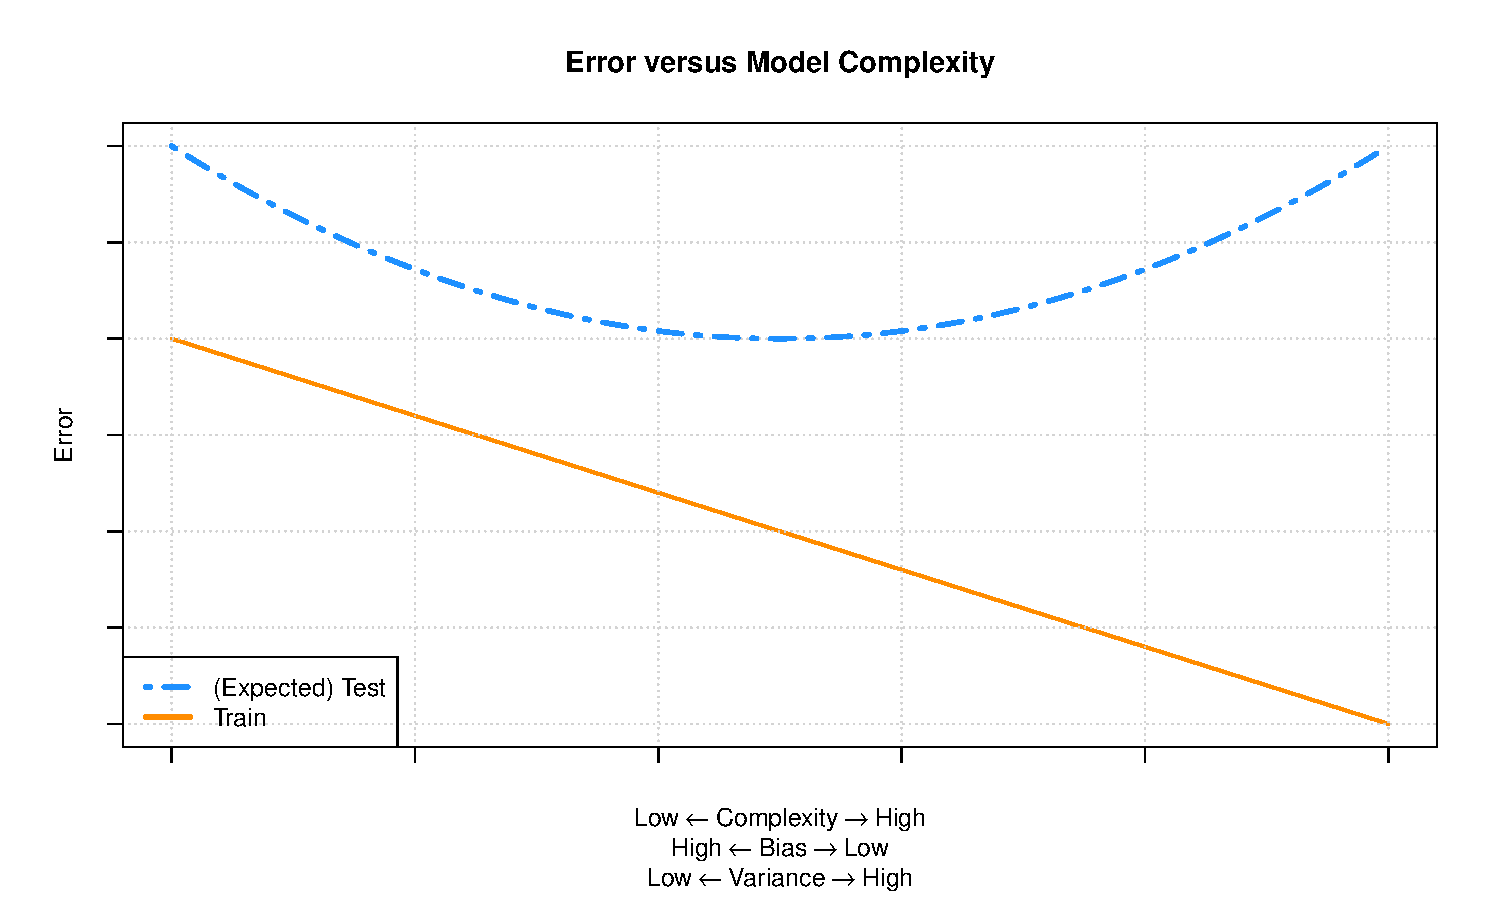
\includegraphics{MyBook_files/figure-latex/unnamed-chunk-97-1.pdf}
Interpretation: The influence is neutral.

\begin{Shaded}
\begin{Highlighting}[]
\NormalTok{b =}\StringTok{ }\DecValTok{6} \OperatorTok{-}\StringTok{ }\DecValTok{6} \OperatorTok{*}\StringTok{ }\NormalTok{x }\OperatorTok{^}\StringTok{ }\NormalTok{(}\DecValTok{1} \OperatorTok{/}\StringTok{ }\DecValTok{4}\NormalTok{)}
\NormalTok{v =}\StringTok{ }\DecValTok{5} \OperatorTok{*}\StringTok{ }\NormalTok{x }\OperatorTok{^}\StringTok{ }\DecValTok{6} \OperatorTok{+}\StringTok{ }\FloatTok{0.5}
\NormalTok{bayes =}\StringTok{ }\DecValTok{4}
\NormalTok{epe =}\StringTok{ }\NormalTok{b }\OperatorTok{+}\StringTok{ }\NormalTok{v }\OperatorTok{+}\StringTok{ }\NormalTok{bayes}

\KeywordTok{plot}\NormalTok{(x, b, }\DataTypeTok{type =} \StringTok{"l"}\NormalTok{, }\DataTypeTok{ylim =} \KeywordTok{c}\NormalTok{(}\DecValTok{0}\NormalTok{, }\DecValTok{10}\NormalTok{), }\DataTypeTok{col =} \StringTok{"dodgerblue"}\NormalTok{, }\DataTypeTok{lwd =} \DecValTok{2}\NormalTok{, }\DataTypeTok{lty =} \DecValTok{3}\NormalTok{,}
     \DataTypeTok{xlab =} \StringTok{"Model Complexity"}\NormalTok{, }\DataTypeTok{ylab =} \StringTok{"Error"}\NormalTok{, }\DataTypeTok{axes =} \OtherTok{FALSE}\NormalTok{,}
     \DataTypeTok{main =} \StringTok{"More Dominant Bias"}\NormalTok{)}
\KeywordTok{axis}\NormalTok{(}\DecValTok{1}\NormalTok{, }\DataTypeTok{labels =} \OtherTok{FALSE}\NormalTok{)}
\KeywordTok{axis}\NormalTok{(}\DecValTok{2}\NormalTok{, }\DataTypeTok{labels =} \OtherTok{FALSE}\NormalTok{)}
\KeywordTok{grid}\NormalTok{()}
\KeywordTok{box}\NormalTok{()}
\KeywordTok{lines}\NormalTok{(x, v, }\DataTypeTok{col =} \StringTok{"darkorange"}\NormalTok{, }\DataTypeTok{lwd =} \DecValTok{2}\NormalTok{, }\DataTypeTok{lty =} \DecValTok{4}\NormalTok{)}
\KeywordTok{lines}\NormalTok{(x, epe, }\DataTypeTok{col =} \StringTok{"black"}\NormalTok{, }\DataTypeTok{lwd =} \DecValTok{2}\NormalTok{)}
\KeywordTok{abline}\NormalTok{(}\DataTypeTok{h =}\NormalTok{ bayes, }\DataTypeTok{lty =} \DecValTok{2}\NormalTok{, }\DataTypeTok{lwd =} \DecValTok{2}\NormalTok{, }\DataTypeTok{col =} \StringTok{"darkgrey"}\NormalTok{)}
\KeywordTok{abline}\NormalTok{(}\DataTypeTok{v =}\NormalTok{ x[}\KeywordTok{which.min}\NormalTok{(epe)], }\DataTypeTok{col =} \StringTok{"grey"}\NormalTok{, }\DataTypeTok{lty =} \DecValTok{3}\NormalTok{, }\DataTypeTok{lwd =} \DecValTok{2}\NormalTok{)}
\KeywordTok{legend}\NormalTok{(}\StringTok{"topright"}\NormalTok{, }\KeywordTok{c}\NormalTok{(}\StringTok{"Squared Bias"}\NormalTok{, }\StringTok{"Variance"}\NormalTok{, }\StringTok{"Bayes"}\NormalTok{, }\StringTok{"EPE"}\NormalTok{), }\DataTypeTok{lty =} \KeywordTok{c}\NormalTok{(}\DecValTok{3}\NormalTok{, }\DecValTok{4}\NormalTok{, }\DecValTok{2}\NormalTok{, }\DecValTok{1}\NormalTok{),}
       \DataTypeTok{col =} \KeywordTok{c}\NormalTok{(}\StringTok{"dodgerblue"}\NormalTok{, }\StringTok{"darkorange"}\NormalTok{, }\StringTok{"darkgrey"}\NormalTok{, }\StringTok{"black"}\NormalTok{), }\DataTypeTok{lwd =} \DecValTok{2}\NormalTok{)}
\end{Highlighting}
\end{Shaded}

\includegraphics{MyBook_files/figure-latex/unnamed-chunk-98-1.pdf}
Interpreatation: The variance influenced the bias more than the expected
prediction error.

In all three examples, the difference between the Bayer error, which is
the horizontal dashed grey line, and the expected prediction, which is
representet by the solid black curve, is exactly the mean squared error,
which is the sum of the squared bias (blue curve) and the vairance
(orange curve). The vertical line represents the complexity that
minimized the prediction error.

It is suposed that the irreducible error can be written as: \[
\mathbb{V}[Y \mid X = x] = \sigma ^ 2
\] Hence, it full decomposition of the expected prediction error of
predicting \(Y\) using \(\hat{f}\) when \(X = x\) can be written as:

\[
\text{EPE}\left(Y, \hat{f}(x)\right) =  
\underbrace{\text{bias}^2\left(\hat{f}(x)\right) + \text{var}\left(\hat{f}(x)\right)}_\textrm{reducible error} + \sigma^2.
\] In summary it can be said that when the model complexity increeases,
the bias decreases, while the variance increases. Therefore,
understanding the tradeoff between bias and variance, the model
complexity can be manipulated in order to find a model which predicts
well on unseen observations.

\includegraphics{MyBook_files/figure-latex/unnamed-chunk-99-1.pdf}

\section{Simulation}\label{simulation}

The decompositions, as well as the bias-variance tradeoff, can be
illustrated through simulation. Assuming that a train model should learn
the true regression function \(f(x) = x^2\).

\begin{Shaded}
\begin{Highlighting}[]
\NormalTok{f =}\StringTok{ }\ControlFlowTok{function}\NormalTok{(x) \{}
\NormalTok{  x }\OperatorTok{^}\StringTok{ }\DecValTok{2}
\NormalTok{\}}
\end{Highlighting}
\end{Shaded}

In particular, an observation \(Y\) should be predicted, given \(X = x\)
by using \(\hat{f}(x)\) where

\[
\mathbb{E}[Y \mid X = x] = f(x) = x^2
\] and

\[
\mathbb{V}[Y \mid X = x] = \sigma ^ 2.
\]

Alternatively, this can be written as

\[
Y = f(X) + \epsilon
\]

where \(\mathbb{E}[\epsilon] = 0\) and
\(\mathbb{V}[\epsilon] = \sigma ^ 2\). In this formulation, \(f(X)\) is
called the \textbf{signal} and \(\epsilon\) the \textbf{noise}.

In order to extradite a specific simulation example, the data
genaerating process need to be fully specfied:

\begin{Shaded}
\begin{Highlighting}[]
\NormalTok{get_sim_data =}\StringTok{ }\ControlFlowTok{function}\NormalTok{(f, }\DataTypeTok{sample_size =} \DecValTok{100}\NormalTok{) \{}
\NormalTok{  x =}\StringTok{ }\KeywordTok{runif}\NormalTok{(}\DataTypeTok{n =}\NormalTok{ sample_size, }\DataTypeTok{min =} \DecValTok{0}\NormalTok{, }\DataTypeTok{max =} \DecValTok{1}\NormalTok{)}
\NormalTok{  y =}\StringTok{ }\KeywordTok{rnorm}\NormalTok{(}\DataTypeTok{n =}\NormalTok{ sample_size, }\DataTypeTok{mean =} \KeywordTok{f}\NormalTok{(x), }\DataTypeTok{sd =} \FloatTok{0.3}\NormalTok{)}
  \KeywordTok{data.frame}\NormalTok{(x, y)}
\NormalTok{\}}
\end{Highlighting}
\end{Shaded}

Note: If it is prefered to think if this simulation using the
\(Y = f(X) + \epsilon\) formulation, the following code represents the
same data generating process.

\begin{Shaded}
\begin{Highlighting}[]
\NormalTok{get_sim_data =}\StringTok{ }\ControlFlowTok{function}\NormalTok{(f, }\DataTypeTok{sample_size =} \DecValTok{100}\NormalTok{) \{}
\NormalTok{  x =}\StringTok{ }\KeywordTok{runif}\NormalTok{(}\DataTypeTok{n =}\NormalTok{ sample_size, }\DataTypeTok{min =} \DecValTok{0}\NormalTok{, }\DataTypeTok{max =} \DecValTok{1}\NormalTok{)}
\NormalTok{  eps =}\StringTok{ }\KeywordTok{rnorm}\NormalTok{(}\DataTypeTok{n =}\NormalTok{ sample_size, }\DataTypeTok{mean =} \DecValTok{0}\NormalTok{, }\DataTypeTok{sd =} \FloatTok{0.75}\NormalTok{)}
\NormalTok{  y =}\StringTok{ }\KeywordTok{f}\NormalTok{(x) }\OperatorTok{+}\StringTok{ }\NormalTok{eps}
  \KeywordTok{data.frame}\NormalTok{(x, y)}
\NormalTok{\}}
\end{Highlighting}
\end{Shaded}

In order to completely specify the data generating process, more model
assumptions has to be made than simply
\(\mathbb{E}[Y \mid X = x] = x^2\) and
\(\mathbb{V}[Y \mid X = x] = \sigma ^ 2\). In particular,

\begin{itemize}
\tightlist
\item
  The \(x_i\) in \(\mathcal{D}\) are sampled from a uniform distribution
  over \([0, 1]\).
\item
  The \(x_i\) and \(\epsilon\) are independent.
\item
  The \(y_i\) in \(\mathcal{D}\) are sampled from the conditional normal
  distribution.
\end{itemize}

\[
Y \mid X \sim N(f(x), \sigma^2)
\]

For obtaining this setup, the datasets \(\mathcal{D}\) will be generated
with a sample size \(n = 100\) and fit four models.

\[
\begin{aligned}
\texttt{predict(fit0, x)} &= \hat{f}_0(x) = \hat{\beta}_0\\
\texttt{predict(fit1, x)} &= \hat{f}_1(x) = \hat{\beta}_0 + \hat{\beta}_1 x \\
\texttt{predict(fit2, x)} &= \hat{f}_2(x) = \hat{\beta}_0 + \hat{\beta}_1 x + \hat{\beta}_2 x^2 \\
\texttt{predict(fit9, x)} &= \hat{f}_9(x) = \hat{\beta}_0 + \hat{\beta}_1 x + \hat{\beta}_2 x^2 + \ldots + \hat{\beta}_9 x^9
\end{aligned}
\] For making use of the data and the four models, a simulated dataset
is generated, and fit the four models.

\begin{Shaded}
\begin{Highlighting}[]
\KeywordTok{set.seed}\NormalTok{(}\DecValTok{1}\NormalTok{)}
\NormalTok{sim_data =}\StringTok{ }\KeywordTok{get_sim_data}\NormalTok{(f)}
\end{Highlighting}
\end{Shaded}

\begin{Shaded}
\begin{Highlighting}[]
\NormalTok{fit_}\DecValTok{0}\NormalTok{ =}\StringTok{ }\KeywordTok{lm}\NormalTok{(y }\OperatorTok{~}\StringTok{ }\DecValTok{1}\NormalTok{,                   }\DataTypeTok{data =}\NormalTok{ sim_data)}
\NormalTok{fit_}\DecValTok{1}\NormalTok{ =}\StringTok{ }\KeywordTok{lm}\NormalTok{(y }\OperatorTok{~}\StringTok{ }\KeywordTok{poly}\NormalTok{(x, }\DataTypeTok{degree =} \DecValTok{1}\NormalTok{), }\DataTypeTok{data =}\NormalTok{ sim_data)}
\NormalTok{fit_}\DecValTok{2}\NormalTok{ =}\StringTok{ }\KeywordTok{lm}\NormalTok{(y }\OperatorTok{~}\StringTok{ }\KeywordTok{poly}\NormalTok{(x, }\DataTypeTok{degree =} \DecValTok{2}\NormalTok{), }\DataTypeTok{data =}\NormalTok{ sim_data)}
\NormalTok{fit_}\DecValTok{9}\NormalTok{ =}\StringTok{ }\KeywordTok{lm}\NormalTok{(y }\OperatorTok{~}\StringTok{ }\KeywordTok{poly}\NormalTok{(x, }\DataTypeTok{degree =} \DecValTok{9}\NormalTok{), }\DataTypeTok{data =}\NormalTok{ sim_data)}
\end{Highlighting}
\end{Shaded}

\includegraphics{MyBook_files/figure-latex/unnamed-chunk-106-1.pdf}
Interpretation: When plotting the four trained models, it can be seen
that the zero predictor models does very bad. The first degree mdeol is
reasonabale, but it can be seen that second degree model fits much
better. The ninth model seem rather wild.

When staying to the three plots which are created when using three
further simulated datasets. The zero predictor and nith degree
ploynomial were fit to each.

\begin{Shaded}
\begin{Highlighting}[]
\KeywordTok{plot}\NormalTok{(y }\OperatorTok{~}\StringTok{ }\NormalTok{x, }\DataTypeTok{data =}\NormalTok{ sim_data_}\DecValTok{1}\NormalTok{, }\DataTypeTok{col =} \StringTok{"grey"}\NormalTok{, }\DataTypeTok{pch =} \DecValTok{20}\NormalTok{, }\DataTypeTok{main =} \StringTok{"Simulated Dataset 1"}\NormalTok{)}
\KeywordTok{grid}\NormalTok{()}
\NormalTok{grid =}\StringTok{ }\KeywordTok{seq}\NormalTok{(}\DataTypeTok{from =} \DecValTok{0}\NormalTok{, }\DataTypeTok{to =} \DecValTok{2}\NormalTok{, }\DataTypeTok{by =} \FloatTok{0.01}\NormalTok{)}
\KeywordTok{lines}\NormalTok{(grid, }\KeywordTok{predict}\NormalTok{(fit_0_}\DecValTok{1}\NormalTok{, }\DataTypeTok{newdata =} \KeywordTok{data.frame}\NormalTok{(}\DataTypeTok{x =}\NormalTok{ grid)), }\DataTypeTok{col =} \StringTok{"dodgerblue"}\NormalTok{, }\DataTypeTok{lwd =} \DecValTok{2}\NormalTok{, }\DataTypeTok{lty =} \DecValTok{2}\NormalTok{)}
\KeywordTok{lines}\NormalTok{(grid, }\KeywordTok{predict}\NormalTok{(fit_9_}\DecValTok{1}\NormalTok{, }\DataTypeTok{newdata =} \KeywordTok{data.frame}\NormalTok{(}\DataTypeTok{x =}\NormalTok{ grid)), }\DataTypeTok{col =} \StringTok{"darkorange"}\NormalTok{, }\DataTypeTok{lwd =} \DecValTok{2}\NormalTok{, }\DataTypeTok{lty =} \DecValTok{5}\NormalTok{)}
\KeywordTok{legend}\NormalTok{(}\StringTok{"topleft"}\NormalTok{, }\KeywordTok{c}\NormalTok{(}\StringTok{"y ~ 1"}\NormalTok{, }\StringTok{"y ~ poly(x, 9)"}\NormalTok{), }\DataTypeTok{col =} \KeywordTok{c}\NormalTok{(}\StringTok{"dodgerblue"}\NormalTok{, }\StringTok{"darkorange"}\NormalTok{), }\DataTypeTok{lty =} \KeywordTok{c}\NormalTok{(}\DecValTok{2}\NormalTok{, }\DecValTok{5}\NormalTok{), }\DataTypeTok{lwd =} \DecValTok{2}\NormalTok{)}
\end{Highlighting}
\end{Shaded}

\includegraphics{MyBook_files/figure-latex/unnamed-chunk-108-1.pdf}

\begin{Shaded}
\begin{Highlighting}[]
\KeywordTok{plot}\NormalTok{(y }\OperatorTok{~}\StringTok{ }\NormalTok{x, }\DataTypeTok{data =}\NormalTok{ sim_data_}\DecValTok{2}\NormalTok{, }\DataTypeTok{col =} \StringTok{"grey"}\NormalTok{, }\DataTypeTok{pch =} \DecValTok{20}\NormalTok{, }\DataTypeTok{main =} \StringTok{"Simulated Dataset 2"}\NormalTok{)}
\KeywordTok{grid}\NormalTok{()}
\NormalTok{grid =}\StringTok{ }\KeywordTok{seq}\NormalTok{(}\DataTypeTok{from =} \DecValTok{0}\NormalTok{, }\DataTypeTok{to =} \DecValTok{2}\NormalTok{, }\DataTypeTok{by =} \FloatTok{0.01}\NormalTok{)}
\KeywordTok{lines}\NormalTok{(grid, }\KeywordTok{predict}\NormalTok{(fit_0_}\DecValTok{2}\NormalTok{, }\DataTypeTok{newdata =} \KeywordTok{data.frame}\NormalTok{(}\DataTypeTok{x =}\NormalTok{ grid)), }\DataTypeTok{col =} \StringTok{"dodgerblue"}\NormalTok{, }\DataTypeTok{lwd =} \DecValTok{2}\NormalTok{, }\DataTypeTok{lty =} \DecValTok{2}\NormalTok{)}
\KeywordTok{lines}\NormalTok{(grid, }\KeywordTok{predict}\NormalTok{(fit_9_}\DecValTok{2}\NormalTok{, }\DataTypeTok{newdata =} \KeywordTok{data.frame}\NormalTok{(}\DataTypeTok{x =}\NormalTok{ grid)), }\DataTypeTok{col =} \StringTok{"darkorange"}\NormalTok{, }\DataTypeTok{lwd =} \DecValTok{2}\NormalTok{, }\DataTypeTok{lty =} \DecValTok{5}\NormalTok{)}
\KeywordTok{legend}\NormalTok{(}\StringTok{"topleft"}\NormalTok{, }\KeywordTok{c}\NormalTok{(}\StringTok{"y ~ 1"}\NormalTok{, }\StringTok{"y ~ poly(x, 9)"}\NormalTok{), }\DataTypeTok{col =} \KeywordTok{c}\NormalTok{(}\StringTok{"dodgerblue"}\NormalTok{, }\StringTok{"darkorange"}\NormalTok{), }\DataTypeTok{lty =} \KeywordTok{c}\NormalTok{(}\DecValTok{2}\NormalTok{, }\DecValTok{5}\NormalTok{), }\DataTypeTok{lwd =} \DecValTok{2}\NormalTok{)}
\end{Highlighting}
\end{Shaded}

\includegraphics{MyBook_files/figure-latex/unnamed-chunk-109-1.pdf}

\begin{Shaded}
\begin{Highlighting}[]
\KeywordTok{plot}\NormalTok{(y }\OperatorTok{~}\StringTok{ }\NormalTok{x, }\DataTypeTok{data =}\NormalTok{ sim_data_}\DecValTok{3}\NormalTok{, }\DataTypeTok{col =} \StringTok{"grey"}\NormalTok{, }\DataTypeTok{pch =} \DecValTok{20}\NormalTok{, }\DataTypeTok{main =} \StringTok{"Simulated Dataset 3"}\NormalTok{)}
\KeywordTok{grid}\NormalTok{()}
\NormalTok{grid =}\StringTok{ }\KeywordTok{seq}\NormalTok{(}\DataTypeTok{from =} \DecValTok{0}\NormalTok{, }\DataTypeTok{to =} \DecValTok{2}\NormalTok{, }\DataTypeTok{by =} \FloatTok{0.01}\NormalTok{)}
\KeywordTok{lines}\NormalTok{(grid, }\KeywordTok{predict}\NormalTok{(fit_0_}\DecValTok{3}\NormalTok{, }\DataTypeTok{newdata =} \KeywordTok{data.frame}\NormalTok{(}\DataTypeTok{x =}\NormalTok{ grid)), }\DataTypeTok{col =} \StringTok{"dodgerblue"}\NormalTok{, }\DataTypeTok{lwd =} \DecValTok{2}\NormalTok{, }\DataTypeTok{lty =} \DecValTok{2}\NormalTok{)}
\KeywordTok{lines}\NormalTok{(grid, }\KeywordTok{predict}\NormalTok{(fit_9_}\DecValTok{3}\NormalTok{, }\DataTypeTok{newdata =} \KeywordTok{data.frame}\NormalTok{(}\DataTypeTok{x =}\NormalTok{ grid)), }\DataTypeTok{col =} \StringTok{"darkorange"}\NormalTok{, }\DataTypeTok{lwd =} \DecValTok{2}\NormalTok{, }\DataTypeTok{lty =} \DecValTok{5}\NormalTok{)}
\KeywordTok{legend}\NormalTok{(}\StringTok{"topleft"}\NormalTok{, }\KeywordTok{c}\NormalTok{(}\StringTok{"y ~ 1"}\NormalTok{, }\StringTok{"y ~ poly(x, 9)"}\NormalTok{), }\DataTypeTok{col =} \KeywordTok{c}\NormalTok{(}\StringTok{"dodgerblue"}\NormalTok{, }\StringTok{"darkorange"}\NormalTok{), }\DataTypeTok{lty =} \KeywordTok{c}\NormalTok{(}\DecValTok{2}\NormalTok{, }\DecValTok{5}\NormalTok{), }\DataTypeTok{lwd =} \DecValTok{2}\NormalTok{)}
\end{Highlighting}
\end{Shaded}

\includegraphics{MyBook_files/figure-latex/unnamed-chunk-110-1.pdf}

Interpretation: The plots make straighten out the difference between the
bias and variance of these two models. The zero predictor model is
clearly wrong, that is, biased, but nearly the same for each of the
datasets, since it has very low variance.

While the ninth degree model does not appear to be correct for any of
these three simulations, it can be seen that on average it is, and thus
is performing unbiased estimation. These plots do however clearly
illustrate that the ninth degree polynomial is extremely variable. Each
dataset results in a very different fitted model. Correct on average is
not the only goal that after, since in practice, only a single dataset
is used. This is why also the models like to exhibit low variance.

In this case, it can be seen that when \(k\) = 100, it is a biased model
with very low variance. When \(k\) = 5, it is again a highly variable
model.

These two sets of plots reinforce the intuition about the bias-variance
tradeoff. Complex models (ninth degree polynomial and \(k\) = 5) are
highly variable, and often unbiased. Simple models (zero predictor
linear model and \(k = 100\)) are very biased, but have extremely low
variance.

\chapter{Classification}\label{classification}

Classification is also a form of supervised learning. Here, the response
variable is categorical, as opposed to numeric for regression. The goal
is to find a rule, algorithm, or a function which takes as input a
feature vector, and outputs a category which is the true category as
often as possible. (David Dalpiaz)

That is, the classifier \(\hat{C}(x)\) returns the predicted category
\(\hat{y}(X)\).

\[\hat{y}(x) = \hat{C}(x)\]

\begin{itemize}
\tightlist
\item
  Qualitative variables take values in an unordered set C, such as email
  \{spam, ham\}.
\item
  Given a feature vector X and a qualitative response Y taking values in
  the set C, the classification task is to build a function C(X) that
  takes as input the feature vector X and predicts value; i.e.~C(X)E C.
\item
  Often we are more interested in estimating the probabilities that X
  belongs to each category in C.
\end{itemize}

For example, it is more valuable to have an estimate of the probability
that an insurance claim is fraudulent, than a classification fraudulent
or not.

In order to build the first classifier, the Default dataset from the
ISLR package is used.

\begin{Shaded}
\begin{Highlighting}[]
\KeywordTok{library}\NormalTok{(ISLR)}
\KeywordTok{library}\NormalTok{(tibble)}
\KeywordTok{as_tibble}\NormalTok{(Default)}
\end{Highlighting}
\end{Shaded}

\begin{verbatim}
## # A tibble: 10,000 x 4
##    default student balance income
##    <fct>   <fct>     <dbl>  <dbl>
##  1 No      No         730. 44362.
##  2 No      Yes        817. 12106.
##  3 No      No        1074. 31767.
##  4 No      No         529. 35704.
##  5 No      No         786. 38463.
##  6 No      Yes        920.  7492.
##  7 No      No         826. 24905.
##  8 No      Yes        809. 17600.
##  9 No      No        1161. 37469.
## 10 No      No           0  29275.
## # ... with 9,990 more rows
\end{verbatim}

The goal is to decently classify individuals as defaulters based on
student status, credit card balance, and income. Note: The response
default is the factor, as is the predictor student.

\begin{Shaded}
\begin{Highlighting}[]
\KeywordTok{is.factor}\NormalTok{(Default}\OperatorTok{$}\NormalTok{default)}
\end{Highlighting}
\end{Shaded}

\begin{verbatim}
## [1] TRUE
\end{verbatim}

\begin{Shaded}
\begin{Highlighting}[]
\KeywordTok{is.factor}\NormalTok{(Default}\OperatorTok{$}\NormalTok{student)}
\end{Highlighting}
\end{Shaded}

\begin{verbatim}
## [1] TRUE
\end{verbatim}

As done previous chaper regression, the data is splitted into test and
train. In this example, 50 \% each are used.

\begin{Shaded}
\begin{Highlighting}[]
\KeywordTok{set.seed}\NormalTok{(}\DecValTok{42}\NormalTok{)}
\NormalTok{default_idx   =}\StringTok{ }\KeywordTok{sample}\NormalTok{(}\KeywordTok{nrow}\NormalTok{(Default), }\DecValTok{5000}\NormalTok{)}
\NormalTok{default_trn =}\StringTok{ }\NormalTok{Default[default_idx, ]}
\NormalTok{default_tst =}\StringTok{ }\NormalTok{Default[}\OperatorTok{-}\NormalTok{default_idx, ]}
\end{Highlighting}
\end{Shaded}

\section{Classification
Visualization}\label{classification-visualization}

Simple classification rules can be used for simple visualizations. In
order to create effective visualizations, the function featurePlot ()
from the package caret () is used.

\begin{Shaded}
\begin{Highlighting}[]
\KeywordTok{library}\NormalTok{(caret)}
\end{Highlighting}
\end{Shaded}

Based on a numerica predictor, a density plot can often suggest a simple
split. Essentially this plot graphs a density estimate

\[\hat{f}_{X_i}(x_i \mid Y = k)\]

for each numeric predictor \(x_i\) and each category \(k\) of the
response \(y\).

\begin{Shaded}
\begin{Highlighting}[]
\KeywordTok{featurePlot}\NormalTok{(}\DataTypeTok{x =}\NormalTok{ default_trn[, }\KeywordTok{c}\NormalTok{(}\StringTok{"balance"}\NormalTok{, }\StringTok{"income"}\NormalTok{)], }
            \DataTypeTok{y =}\NormalTok{ default_trn}\OperatorTok{$}\NormalTok{default,}
            \DataTypeTok{plot =} \StringTok{"density"}\NormalTok{, }
            \DataTypeTok{scales =} \KeywordTok{list}\NormalTok{(}\DataTypeTok{x =} \KeywordTok{list}\NormalTok{(}\DataTypeTok{relation =} \StringTok{"free"}\NormalTok{), }
                          \DataTypeTok{y =} \KeywordTok{list}\NormalTok{(}\DataTypeTok{relation =} \StringTok{"free"}\NormalTok{)), }
            \DataTypeTok{adjust =} \FloatTok{1.5}\NormalTok{, }
            \DataTypeTok{pch =} \StringTok{"|"}\NormalTok{, }
            \DataTypeTok{layout =} \KeywordTok{c}\NormalTok{(}\DecValTok{2}\NormalTok{, }\DecValTok{1}\NormalTok{), }
            \DataTypeTok{auto.key =} \KeywordTok{list}\NormalTok{(}\DataTypeTok{columns =} \DecValTok{2}\NormalTok{))}
\end{Highlighting}
\end{Shaded}

\includegraphics{MyBook_files/figure-latex/unnamed-chunk-115-1.pdf}

Some notes about the arguments to this function according to David
Dalpiaz:

\begin{itemize}
\tightlist
\item
  \texttt{x} is a data frame containing only \textbf{numeric
  predictors}. It would be nonsensical to estimate a density for a
  categorical predictor.
\item
  \texttt{y} is the response variable. It needs to be a factor variable.
  If coded as \texttt{0} and \texttt{1}, you will need to coerce to
  factor for plotting.
\item
  \texttt{plot} specifies the type of plot, here \texttt{density}.
\item
  \texttt{scales} defines the scale of the axes for each plot. By
  default, the axis of each plot would be the same, which often is not
  useful, so the arguments here, a different axis for each plot, will
  almost always be used.
\item
  \texttt{adjust} specifies the amount of smoothing used for the density
  estimate.
\item
  \texttt{pch} specifies the \textbf{p}lot \textbf{ch}aracter used for
  the bottom of the plot.
\item
  \texttt{layout} places the individual plots into rows and columns. For
  some odd reason, it is given as (col, row).
\item
  \texttt{auto.key} defines the key at the top of the plot. The number
  of columns should be the number of categories.
\end{itemize}

It can be seems that the income variable by itself is not peculiarly
effective. However, there seems to be a big difference in default status
at a \texttt{balance} of about 1400. This information will be used
shortly.

\begin{Shaded}
\begin{Highlighting}[]
\KeywordTok{featurePlot}\NormalTok{(}\DataTypeTok{x =}\NormalTok{ default_trn[, }\KeywordTok{c}\NormalTok{(}\StringTok{"balance"}\NormalTok{, }\StringTok{"income"}\NormalTok{)], }
            \DataTypeTok{y =}\NormalTok{ default_trn}\OperatorTok{$}\NormalTok{student,}
            \DataTypeTok{plot =} \StringTok{"density"}\NormalTok{, }
            \DataTypeTok{scales =} \KeywordTok{list}\NormalTok{(}\DataTypeTok{x =} \KeywordTok{list}\NormalTok{(}\DataTypeTok{relation =} \StringTok{"free"}\NormalTok{), }
                          \DataTypeTok{y =} \KeywordTok{list}\NormalTok{(}\DataTypeTok{relation =} \StringTok{"free"}\NormalTok{)), }
            \DataTypeTok{adjust =} \FloatTok{1.5}\NormalTok{, }
            \DataTypeTok{pch =} \StringTok{"|"}\NormalTok{, }
            \DataTypeTok{layout =} \KeywordTok{c}\NormalTok{(}\DecValTok{2}\NormalTok{, }\DecValTok{1}\NormalTok{), }
            \DataTypeTok{auto.key =} \KeywordTok{list}\NormalTok{(}\DataTypeTok{columns =} \DecValTok{2}\NormalTok{))}
\end{Highlighting}
\end{Shaded}

\includegraphics{MyBook_files/figure-latex/unnamed-chunk-116-1.pdf}

A similar plot is created, except with \texttt{student} as the response.
It can be seen that students often carry a slightly larger balance, and
have far lower income. This will be useful to know when making more
complicated classifiers.

\begin{Shaded}
\begin{Highlighting}[]
\KeywordTok{featurePlot}\NormalTok{(}\DataTypeTok{x =}\NormalTok{ default_trn[, }\KeywordTok{c}\NormalTok{(}\StringTok{"student"}\NormalTok{, }\StringTok{"balance"}\NormalTok{, }\StringTok{"income"}\NormalTok{)], }
            \DataTypeTok{y =}\NormalTok{ default_trn}\OperatorTok{$}\NormalTok{default, }
            \DataTypeTok{plot =} \StringTok{"pairs"}\NormalTok{,}
            \DataTypeTok{auto.key =} \KeywordTok{list}\NormalTok{(}\DataTypeTok{columns =} \DecValTok{2}\NormalTok{))}
\end{Highlighting}
\end{Shaded}

\includegraphics{MyBook_files/figure-latex/unnamed-chunk-117-1.pdf}

\texttt{plot\ =\ "pairs"} can be used to consider multiple variables at
the same time. This plot reinforces using \texttt{balance} to create a
classifier, and again shows that \texttt{income} seems not that useful.

\begin{Shaded}
\begin{Highlighting}[]
\KeywordTok{library}\NormalTok{(ellipse)}
\KeywordTok{featurePlot}\NormalTok{(}\DataTypeTok{x =}\NormalTok{ default_trn[, }\KeywordTok{c}\NormalTok{(}\StringTok{"balance"}\NormalTok{, }\StringTok{"income"}\NormalTok{)], }
            \DataTypeTok{y =}\NormalTok{ default_trn}\OperatorTok{$}\NormalTok{default, }
            \DataTypeTok{plot =} \StringTok{"ellipse"}\NormalTok{,}
            \DataTypeTok{auto.key =} \KeywordTok{list}\NormalTok{(}\DataTypeTok{columns =} \DecValTok{2}\NormalTok{))}
\end{Highlighting}
\end{Shaded}

\includegraphics{MyBook_files/figure-latex/unnamed-chunk-118-1.pdf}

Similar to \texttt{pairs} is a plot of type \texttt{ellipse}, which
requires the \texttt{ellipse} package. Here we only use numeric
predictors, as essentially we are assuming multivariate normality. The
ellipses mark points of equal density. This will be useful later when
discussing LDA and QDA.

Example: Credit Card Default

\begin{Shaded}
\begin{Highlighting}[]
\NormalTok{show.index <-}\StringTok{ }\KeywordTok{sample}\NormalTok{(}\DecValTok{1}\OperatorTok{:}\KeywordTok{nrow}\NormalTok{(Default), }\DecValTok{1000}\NormalTok{)}

\KeywordTok{plot}\NormalTok{(Default}\OperatorTok{$}\NormalTok{balance[show.index], }
\NormalTok{Default}\OperatorTok{$}\NormalTok{income[show.index], }\DataTypeTok{col =}
\NormalTok{Default}\OperatorTok{$}\NormalTok{default[show.index])}
\end{Highlighting}
\end{Shaded}

\includegraphics{MyBook_files/figure-latex/unnamed-chunk-119-1.pdf}

\begin{Shaded}
\begin{Highlighting}[]
\KeywordTok{boxplot}\NormalTok{(Default}\OperatorTok{$}\NormalTok{balance }\OperatorTok{~}\StringTok{ }\NormalTok{Default}\OperatorTok{$}\NormalTok{default)}
\end{Highlighting}
\end{Shaded}

\includegraphics{MyBook_files/figure-latex/unnamed-chunk-119-2.pdf}

\section{Can we use Linear
Regression?}\label{can-we-use-linear-regression}

Supposing for the Default classification task that it is coded

\[{Y} = 
\begin{cases} 
      0 & if \ no \\
      1 & if \ yes
\end{cases}\]

Can a simple linear regresssion of Y on X can be performed and classify
as Yes if \(\hat{Y} > 0.5\)?

\begin{itemize}
\tightlist
\item
  In this case of a binary outcome, linear regression does a good job as
  a classifier, and is equivalent to linear discriminat analysis which
  is discussed in a later.
\item
  Since in the population
  \[\mathbb{E}[Y \mid X = x] = P(Y = 1 \mid X = x).\] it might be
  thinking that regression is perfect for this task.
\item
  However, linaer regression might produce probabilities less than zero
  or bigger than one. Logistic regression is more appropriate.
\end{itemize}

\section{Linear versus Logistic
Regression}\label{linear-versus-logistic-regression}

\begin{Shaded}
\begin{Highlighting}[]
\NormalTok{default_trn_lm =}\StringTok{ }\NormalTok{default_trn}
\NormalTok{default_tst_lm =}\StringTok{ }\NormalTok{default_tst}
\end{Highlighting}
\end{Shaded}

\begin{Shaded}
\begin{Highlighting}[]
\NormalTok{default_trn_lm}\OperatorTok{$}\NormalTok{default =}\StringTok{ }\KeywordTok{as.numeric}\NormalTok{(default_trn_lm}\OperatorTok{$}\NormalTok{default) }\OperatorTok{-}\StringTok{ }\DecValTok{1}
\NormalTok{default_tst_lm}\OperatorTok{$}\NormalTok{default =}\StringTok{ }\KeywordTok{as.numeric}\NormalTok{(default_tst_lm}\OperatorTok{$}\NormalTok{default) }\OperatorTok{-}\StringTok{ }\DecValTok{1}
\end{Highlighting}
\end{Shaded}

\begin{Shaded}
\begin{Highlighting}[]
\NormalTok{model_lm =}\StringTok{ }\KeywordTok{lm}\NormalTok{(default }\OperatorTok{~}\StringTok{ }\NormalTok{balance, }\DataTypeTok{data =}\NormalTok{ default_trn_lm)}
\end{Highlighting}
\end{Shaded}

\begin{Shaded}
\begin{Highlighting}[]
\KeywordTok{plot}\NormalTok{(default }\OperatorTok{~}\StringTok{ }\NormalTok{balance, }\DataTypeTok{data =}\NormalTok{ default_trn_lm, }
     \DataTypeTok{col =} \StringTok{"darkorange"}\NormalTok{, }\DataTypeTok{pch =} \StringTok{"|"}\NormalTok{, }\DataTypeTok{ylim =} \KeywordTok{c}\NormalTok{(}\OperatorTok{-}\FloatTok{0.2}\NormalTok{, }\DecValTok{1}\NormalTok{),}
     \DataTypeTok{main =} \StringTok{"Using Linear Regression for Classification"}\NormalTok{)}
\KeywordTok{abline}\NormalTok{(}\DataTypeTok{h =} \DecValTok{0}\NormalTok{, }\DataTypeTok{lty =} \DecValTok{3}\NormalTok{)}
\KeywordTok{abline}\NormalTok{(}\DataTypeTok{h =} \DecValTok{1}\NormalTok{, }\DataTypeTok{lty =} \DecValTok{3}\NormalTok{)}
\KeywordTok{abline}\NormalTok{(}\DataTypeTok{h =} \FloatTok{0.5}\NormalTok{, }\DataTypeTok{lty =} \DecValTok{2}\NormalTok{)}
\KeywordTok{abline}\NormalTok{(model_lm, }\DataTypeTok{lwd =} \DecValTok{3}\NormalTok{, }\DataTypeTok{col =} \StringTok{"dodgerblue"}\NormalTok{)}
\end{Highlighting}
\end{Shaded}

\includegraphics{MyBook_files/figure-latex/unnamed-chunk-123-1.pdf}
Linear regression does not estimate \(P(Y = 1 \mid X = x)\). The graph
of linear regression shows that the predicted probabilities are below
0.5., indicating that every observation would be classified as ```No''
This could be possible, but it is not what is expected.

\begin{Shaded}
\begin{Highlighting}[]
\KeywordTok{all}\NormalTok{(}\KeywordTok{predict}\NormalTok{(model_lm) }\OperatorTok{<}\StringTok{ }\FloatTok{0.5}\NormalTok{)}
\end{Highlighting}
\end{Shaded}

\begin{verbatim}
## [1] TRUE
\end{verbatim}

A further issue is that the predicted probabilty is less than 0.

\begin{Shaded}
\begin{Highlighting}[]
\KeywordTok{any}\NormalTok{(}\KeywordTok{predict}\NormalTok{(model_lm) }\OperatorTok{<}\StringTok{ }\DecValTok{0}\NormalTok{)}
\end{Highlighting}
\end{Shaded}

\begin{verbatim}
## [1] TRUE
\end{verbatim}

\chapter{Logistic regression}\label{logistic-regression}

\[p(x) = P(Y = 1 \mid {X = x})\]

\begin{Shaded}
\begin{Highlighting}[]
\NormalTok{model_glm =}\StringTok{ }\KeywordTok{glm}\NormalTok{(default }\OperatorTok{~}\StringTok{ }\NormalTok{balance, }\DataTypeTok{data =}\NormalTok{ default_trn, }\DataTypeTok{family =} \StringTok{"binomial"}\NormalTok{)}
\end{Highlighting}
\end{Shaded}

\begin{Shaded}
\begin{Highlighting}[]
\KeywordTok{coef}\NormalTok{(model_glm)}
\end{Highlighting}
\end{Shaded}

\begin{verbatim}
##   (Intercept)       balance 
## -10.452182876   0.005367655
\end{verbatim}

\begin{Shaded}
\begin{Highlighting}[]
\KeywordTok{head}\NormalTok{(}\KeywordTok{predict}\NormalTok{(model_glm))}
\end{Highlighting}
\end{Shaded}

\begin{verbatim}
##       9149       9370       2861       8302       6415       5189 
## -6.9616496 -0.7089539 -4.8936916 -9.4123620 -9.0416096 -7.3600645
\end{verbatim}

\begin{Shaded}
\begin{Highlighting}[]
\KeywordTok{head}\NormalTok{(}\KeywordTok{predict}\NormalTok{(model_glm, }\DataTypeTok{type =} \StringTok{"link"}\NormalTok{))}
\end{Highlighting}
\end{Shaded}

\begin{verbatim}
##       9149       9370       2861       8302       6415       5189 
## -6.9616496 -0.7089539 -4.8936916 -9.4123620 -9.0416096 -7.3600645
\end{verbatim}

\begin{Shaded}
\begin{Highlighting}[]
\KeywordTok{head}\NormalTok{(}\KeywordTok{predict}\NormalTok{(model_glm, }\DataTypeTok{type =} \StringTok{"response"}\NormalTok{))}
\end{Highlighting}
\end{Shaded}

\begin{verbatim}
##         9149         9370         2861         8302         6415 
## 9.466353e-04 3.298300e-01 7.437969e-03 8.170105e-05 1.183661e-04 
##         5189 
## 6.357530e-04
\end{verbatim}

\begin{Shaded}
\begin{Highlighting}[]
\NormalTok{calc_class_err =}\StringTok{ }\ControlFlowTok{function}\NormalTok{(actual, predicted) \{}
  \KeywordTok{mean}\NormalTok{(actual }\OperatorTok{!=}\StringTok{ }\NormalTok{predicted)}
\NormalTok{\}}
\end{Highlighting}
\end{Shaded}

\begin{Shaded}
\begin{Highlighting}[]
\CommentTok{#calc_class_err(actual = default_trn$default, predicted = model_glm_pred)}
\end{Highlighting}
\end{Shaded}

Logistic regression is used to better estimate the propability.

The model is

\[\log\left(\frac{p(x)}{1 - p(x)}\right) = \beta_0 + \beta_1 x_1 + \beta_2 x_2 + \cdots  + \beta_p x_p.\]

\begin{Shaded}
\begin{Highlighting}[]
\KeywordTok{plot}\NormalTok{(default }\OperatorTok{~}\StringTok{ }\NormalTok{balance, }\DataTypeTok{data =}\NormalTok{ default_trn_lm, }
     \DataTypeTok{col =} \StringTok{"darkorange"}\NormalTok{, }\DataTypeTok{pch =} \StringTok{"|"}\NormalTok{, }\DataTypeTok{ylim =} \KeywordTok{c}\NormalTok{(}\OperatorTok{-}\FloatTok{0.2}\NormalTok{, }\DecValTok{1}\NormalTok{),}
     \DataTypeTok{main =} \StringTok{"Using Logistic Regression for Classification"}\NormalTok{)}
\KeywordTok{abline}\NormalTok{(}\DataTypeTok{h =} \DecValTok{0}\NormalTok{, }\DataTypeTok{lty =} \DecValTok{3}\NormalTok{)}
\KeywordTok{abline}\NormalTok{(}\DataTypeTok{h =} \DecValTok{1}\NormalTok{, }\DataTypeTok{lty =} \DecValTok{3}\NormalTok{)}
\KeywordTok{abline}\NormalTok{(}\DataTypeTok{h =} \FloatTok{0.5}\NormalTok{, }\DataTypeTok{lty =} \DecValTok{2}\NormalTok{)}
\KeywordTok{curve}\NormalTok{(}\KeywordTok{predict}\NormalTok{(model_glm, }\KeywordTok{data.frame}\NormalTok{(}\DataTypeTok{balance =}\NormalTok{ x), }\DataTypeTok{type =} \StringTok{"response"}\NormalTok{), }
      \DataTypeTok{add =} \OtherTok{TRUE}\NormalTok{, }\DataTypeTok{lwd =} \DecValTok{3}\NormalTok{, }\DataTypeTok{col =} \StringTok{"dodgerblue"}\NormalTok{)}
\KeywordTok{abline}\NormalTok{(}\DataTypeTok{v =} \OperatorTok{-}\KeywordTok{coef}\NormalTok{(model_glm)[}\DecValTok{1}\NormalTok{] }\OperatorTok{/}\StringTok{ }\KeywordTok{coef}\NormalTok{(model_glm)[}\DecValTok{2}\NormalTok{], }\DataTypeTok{lwd =} \DecValTok{2}\NormalTok{)}
\end{Highlighting}
\end{Shaded}

\includegraphics{MyBook_files/figure-latex/unnamed-chunk-133-1.pdf} In
logistic regression it suited well to the task.

This plot contains a wealth of information.

\begin{itemize}
\tightlist
\item
  The orange \texttt{\textbar{}} characters are the data,
  \((x_i, y_i)\).
\item
  The blue ``curve'' is the predicted probabilities given by the fitted
  logistic regression. That is,
  \[\hat{p}(x) = \hat{P}(Y = 1 \mid { X = x})\]
\item
  The solid vertical black line represents the
  \textbf{\href{https://en.wikipedia.org/wiki/Decision_boundary}{decision
  boundary}}, the \texttt{balance} that obtains a predicted probability
  of 0.5. In this case \texttt{balance} = 1947.252994.
\end{itemize}

\chapter{Cross-validation and the
Bootstrap}\label{cross-validation-and-the-bootstrap}

Cross-validation and the bootstrap are two methods of resampling. These
two methods refit a model of interest to samples created from the
training set, for the reason to obtain additional information about the
fitted model. The methods provide estimates of test-set prediction
error, and the standard deviation and bias of the parameter estimates.

\section{Training Error versus Test
error}\label{training-error-versus-test-error}

Here it is useful to recall the distinction between the test error and
the training error. - Test error: average error that results from using
a statistical learning method to predict the response on a new
observation, one that was not used in training the method. - Training
error: can be easily calculated by applying the statistical learning
method to the observations used in its training. - Error rate: the
training error rate can dramatically underestimate the test error rate.

\section{Validation-Set Approach}\label{validation-set-approach}

In the validation-set approach, the available set of samples is divided
into two parts: A training set and a validation or hold-out set. The
model is fit on the training set, and the fitted model is used to
predict the reponse for the observations in the validation set. The
resulting validation-set error provides an estimate of the test error.
This is typically assessed using MSE in the case of a quantitative
reponse and misclassification rate in the case of a qualitative
(discrete) reponse.

Example 1. (with explanations)

In the automobile data example, linear vs.~higher-order polynomial terms
in a linear regression are compared. The 392 observations are splited
into two sets, a training set containing 196 of the data points, and a
validation set containing the remaining 196 observations.

\begin{Shaded}
\begin{Highlighting}[]
\CommentTok{# a function for calculating the RMSE from two vectors}

\NormalTok{c.rmse <-}\StringTok{ }\ControlFlowTok{function}\NormalTok{(observed, predicted)\{}
\NormalTok{  (observed }\OperatorTok{-}\StringTok{ }\NormalTok{predicted)}\OperatorTok{^}\DecValTok{2}\OperatorTok
\StringTok{  }\NormalTok{mean }\OperatorTok
\StringTok{  }\NormalTok{sqrt }\OperatorTok
\StringTok{  }\KeywordTok{round}\NormalTok{(}\DecValTok{3}\NormalTok{)}
\NormalTok{\}}

\NormalTok{c.rmse2 <-}\StringTok{ }\ControlFlowTok{function}\NormalTok{(observed, predicted) \{}
\KeywordTok{round}\NormalTok{(}\KeywordTok{sqrt}\NormalTok{(}\KeywordTok{mean}\NormalTok{((observed }\OperatorTok{-}\NormalTok{predicted)}\OperatorTok{^}\DecValTok{2}\NormalTok{)),}\DecValTok{3}\NormalTok{)}
\NormalTok{\}}
\end{Highlighting}
\end{Shaded}

\begin{Shaded}
\begin{Highlighting}[]
\KeywordTok{require}\NormalTok{(ISLR)}
\KeywordTok{require}\NormalTok{(magrittr)}
\CommentTok{#to load the required packages}

\KeywordTok{set.seed}\NormalTok{(}\DecValTok{43245}\NormalTok{)}
\CommentTok{#in order to create random numbers, but to save this "seed" and not create new random numbers chunks are runned again (as done if put rnorm(41) instead of set.seed}

\CommentTok{#in order to have our training data seperated, we need to half it}

\NormalTok{n <-}\StringTok{ }\KeywordTok{nrow}\NormalTok{(Auto) }
\CommentTok{# just to have an abbreviation}

\NormalTok{train <-}\StringTok{ }\KeywordTok{sample}\NormalTok{(}\DecValTok{1}\OperatorTok{:}\NormalTok{n, }\KeywordTok{ceiling}\NormalTok{(n}\OperatorTok{/}\DecValTok{2}\NormalTok{))}
\CommentTok{#1: to number of rows, ceiling is used to prevent that in case nrow(auto) is odd, you have a number such as 74,3 (also could use round)}

\NormalTok{degrees<-}\StringTok{ }\DecValTok{1}\OperatorTok{:}\DecValTok{10}
\CommentTok{#the different degrees wanted to put in}

\NormalTok{v.rmse <-}\StringTok{ }\KeywordTok{numeric}\NormalTok{ ()}
\CommentTok{#to create a new vector where all values are putted in from the rmse}

\ControlFlowTok{for}\NormalTok{ (i }\ControlFlowTok{in}\NormalTok{ degrees)\{}
\CommentTok{#basically just creating an abbreviation for putting in several polynomals into the fit1}
  
    
\NormalTok{fit1 <-}\StringTok{ }\KeywordTok{glm}\NormalTok{(mpg }\OperatorTok{~}\StringTok{ }\KeywordTok{poly}\NormalTok{(horsepower,i), }\DataTypeTok{data =}\NormalTok{ Auto, }\DataTypeTok{subset =}\NormalTok{ train)}
\NormalTok{  v.rmse[i] <-}
\CommentTok{# fit in into a linear model, in order to create a line that fits the model    }
\NormalTok{v.rmse[i] <-}\StringTok{ }\KeywordTok{c.rmse}\NormalTok{(Auto}\OperatorTok{$}\NormalTok{mpg[}\OperatorTok{-}\NormalTok{train], }\KeywordTok{predict}\NormalTok{(fit1, }\DataTypeTok{newdata=}\NormalTok{Auto[}\OperatorTok{-}\NormalTok{train,]))  }
    
\CommentTok{# how it was before, against what it is now with v.rmse:c.rmse(Auto$mpg[-train], predict(fit1, newdata=Auto[-train,]))}
\CommentTok{#here function is created in order to calculate later the rmse}

\NormalTok{\}}
\CommentTok{# the plot is created to see all the test error values for the different polys (the number after horsepower)}
  

\KeywordTok{plot}\NormalTok{(degrees, v.rmse, }\DataTypeTok{type =}\StringTok{"b"}\NormalTok{, }\DataTypeTok{col =} \StringTok{"red"}\NormalTok{)   }
\end{Highlighting}
\end{Shaded}

\includegraphics{MyBook_files/figure-latex/unnamed-chunk-135-1.pdf}

\begin{Shaded}
\begin{Highlighting}[]
\CommentTok{#type b just shows the type of the line ( can also be l for line or p for points instead of b for both)}
\end{Highlighting}
\end{Shaded}

As a result degree 2 is probably taken, because it is quite good from
its v.rmse and it is not complex (the lower the degree, the better is it
to understand)

In the next step, is is done not just for one split, but multiple
splits:

\begin{Shaded}
\begin{Highlighting}[]
\KeywordTok{require}\NormalTok{(ISLR)}
\KeywordTok{require}\NormalTok{(magrittr)}
\CommentTok{#to load the required packages}

\KeywordTok{set.seed}\NormalTok{(}\DecValTok{120}\NormalTok{)}


\NormalTok{degrees <-}\StringTok{ }\DecValTok{1}\OperatorTok{:}\DecValTok{10}

\NormalTok{n.splits <-}\StringTok{ }\DecValTok{10}

\NormalTok{m.rmse <-}\StringTok{ }\KeywordTok{matrix}\NormalTok{(}\OtherTok{NA}\NormalTok{, }\KeywordTok{length}\NormalTok{(degrees), n.splits)}
\CommentTok{#here NA is the data(numbers), length = number of rows, n.splits = number columns}

\KeywordTok{library}\NormalTok{(ISLR)}

\ControlFlowTok{for}\NormalTok{(s }\ControlFlowTok{in} \DecValTok{1}\OperatorTok{:}\NormalTok{n.splits)\{}
\NormalTok{  train <-}\StringTok{ }\KeywordTok{sample}\NormalTok{(}\DecValTok{1}\OperatorTok{:}\NormalTok{n, }\KeywordTok{ceiling}\NormalTok{(n}\OperatorTok{/}\DecValTok{2}\NormalTok{))}
\ControlFlowTok{for}\NormalTok{(i }\ControlFlowTok{in}\NormalTok{ degrees) \{}
\NormalTok{  fit1<-}\StringTok{ }\KeywordTok{glm}\NormalTok{(mpg }\OperatorTok{~}\StringTok{ }\KeywordTok{poly}\NormalTok{ (horsepower, i), }\DataTypeTok{data =}\NormalTok{ Auto, }\DataTypeTok{subset =}\NormalTok{ train)}
\NormalTok{m.rmse[i,s] <-}\StringTok{ }\KeywordTok{c.rmse}\NormalTok{(Auto}\OperatorTok{$}\NormalTok{mpg[}\OperatorTok{-}\NormalTok{train], }\KeywordTok{predict}\NormalTok{(fit1, }\DataTypeTok{newdata =}\NormalTok{ Auto[}\OperatorTok{-}\NormalTok{train,]))}

\NormalTok{\}}
\NormalTok{\}}
  
\KeywordTok{plot}\NormalTok{(degrees, m.rmse[,}\DecValTok{1}\NormalTok{], }\DataTypeTok{type =}\StringTok{"l"}\NormalTok{, }\DataTypeTok{col =} \StringTok{"red"}\NormalTok{, }\DataTypeTok{ylim=}\KeywordTok{c}\NormalTok{(}\KeywordTok{min}\NormalTok{(m.rmse), }\KeywordTok{max}\NormalTok{(m.rmse)))}
\ControlFlowTok{for}\NormalTok{ (s }\ControlFlowTok{in} \DecValTok{1}\OperatorTok{:}\NormalTok{n.splits)\{}
  \KeywordTok{lines}\NormalTok{(degrees, m.rmse[,s], }\DataTypeTok{col =}\NormalTok{s)}
\NormalTok{\}}
\end{Highlighting}
\end{Shaded}

\includegraphics{MyBook_files/figure-latex/unnamed-chunk-136-1.pdf}

Example 2.

\begin{itemize}
\tightlist
\item
  Consider fitting polynomial models of degree k = 1:10 data from this
  data generating process
\item
  Consider k, the polynomial degree, as a turning parameter how well
  validation set approach works.
\end{itemize}

\begin{Shaded}
\begin{Highlighting}[]
\NormalTok{num_sims =}\StringTok{ }\DecValTok{100}
\NormalTok{num_degrees =}\StringTok{ }\DecValTok{10}
\NormalTok{val_rmse =}\StringTok{ }\KeywordTok{matrix}\NormalTok{(}\DecValTok{0}\NormalTok{, }\DataTypeTok{ncol =}\NormalTok{ num_degrees, }\DataTypeTok{nrow =}\NormalTok{ num_sims)}
\end{Highlighting}
\end{Shaded}

The simulations are:

\begin{Shaded}
\begin{Highlighting}[]
\KeywordTok{set.seed}\NormalTok{(}\DecValTok{42}\NormalTok{)}
\ControlFlowTok{for}\NormalTok{ (i }\ControlFlowTok{in} \DecValTok{1}\OperatorTok{:}\NormalTok{num_sims) \{}
  \CommentTok{# simulate data}
\NormalTok{  sim_data =}\StringTok{ }\KeywordTok{gen_sim_data}\NormalTok{(}\DataTypeTok{sample_size =} \DecValTok{200}\NormalTok{)}
  \CommentTok{# set aside validation set}
\NormalTok{  sim_idx =}\StringTok{ }\KeywordTok{sample}\NormalTok{(}\DecValTok{1}\OperatorTok{:}\KeywordTok{nrow}\NormalTok{(sim_data), }\DecValTok{160}\NormalTok{)}
\NormalTok{  sim_trn =}\StringTok{ }\NormalTok{sim_data[sim_idx, ]}
\NormalTok{  sim_val =}\StringTok{ }\NormalTok{sim_data[}\OperatorTok{-}\NormalTok{sim_idx, ]}
  \CommentTok{# fit models and store RMSEs}
  \ControlFlowTok{for}\NormalTok{ (j }\ControlFlowTok{in} \DecValTok{1}\OperatorTok{:}\NormalTok{num_degrees) \{}
    \CommentTok{#fit model}
\NormalTok{    fit =}\StringTok{ }\KeywordTok{glm}\NormalTok{(y }\OperatorTok{~}\StringTok{ }\KeywordTok{poly}\NormalTok{(x, }\DataTypeTok{degree =}\NormalTok{ j), }\DataTypeTok{data =}\NormalTok{ sim_trn)}
    \CommentTok{# calculate error}
\NormalTok{    val_rmse[i, j] =}\StringTok{ }\KeywordTok{calc_rmse}\NormalTok{(}\DataTypeTok{actual =}\NormalTok{ sim_val}\OperatorTok{$}\NormalTok{y, }\DataTypeTok{predicted =} \KeywordTok{predict}\NormalTok{(fit, sim_val))}
\NormalTok{  \}}
\NormalTok{\}}
\end{Highlighting}
\end{Shaded}

\includegraphics{MyBook_files/figure-latex/unnamed-chunk-143-1.pdf}

\section{Drawbacks of validation set
approach}\label{drawbacks-of-validation-set-approach}

The validation estimate of the test error can be highly variable,
depending on precisely which observations are included in the training
set and which observations can be included in the validation set. In the
validation approach, only a subset of the observations - those that are
included in the training set rather than in the validation set - are
used to fit the model. This suggestes that the validation set error may
tend to overestimate the test error for the model fit on the entire data
set.

\section{K-fold Cross validation}\label{k-fold-cross-validation}

This is a widely used approach for estimating the test error. The
estimtates can be used to select the optimal model and to give an idea
of the test error and the final chosen model. The idea is to randomly
divide the data into K equal-sized parts. The k part is left out, fit
the model to the other predictions for the left-out kth part. This
appears through in turn for ach part k = 1, 2,\ldots{}K, and then the
results are combined.

1 2 3 4 5 Validation Train Train Train Train

\section{The Bootstrap}\label{the-bootstrap}

The bootstrap is another resampling method. It is a flexible and
powerful statistical tool that can be used to quantify the uncertainty
associated with a given estimator or statistical learning method. E.g.
it is usedful for providing an estimate of the standard error of a
coefficient, or a confidence interval for that coefficient. The
bootstrap could be used to replace the cross-validation method, however
it aligns significantly more computation.

\chapter{Tree-based methods}\label{tree-based-methods}

In this chapter, tree-based methods for regression and classification
are discussed. These include stratifying or segmenting the predictor
space into a number of single regions. Since the set of splitting ruls
used to segment the predictor space can be summarized in a tree, these
type pf approaches are known as decision tree methods.

\section{Pro and Cons of Trees}\label{pro-and-cons-of-trees}

One the one hand, tree-based methods are simple and useful for
interpretation. On the other hand, they are typically not competitive
with the best supervised learning approaches in terms of prediction
accuracy. Further methods are bagging, random forest, and boosting,
which grow multiple trees which are then combined to yield a single
consensus prediction. Combining a large number of trees can often result
in dramatic improvements in prediction accuracy, at the expense of some
loss interpretation.

\section{The Basics of Decision
Trees}\label{the-basics-of-decision-trees}

Decision trees can be used to regression and classification problems. In
this chaper, the regression problems are considered first and second the
classification problems

\section{Example}\label{example}

Baseball salaray data: how to stratify it?

\begin{Shaded}
\begin{Highlighting}[]
\KeywordTok{require}\NormalTok{(ggplot2)}

\KeywordTok{data}\NormalTok{(}\StringTok{"Hitters"}\NormalTok{)}

\NormalTok{Hitters  }\OperatorTok
\StringTok{  }\KeywordTok{ggplot}\NormalTok{(}\KeywordTok{aes}\NormalTok{(}\DataTypeTok{x=}\NormalTok{Years, }\DataTypeTok{y=}\NormalTok{Hits, }\DataTypeTok{col=}\NormalTok{Salary)) }\OperatorTok{+}
\StringTok{  }\KeywordTok{geom_point}\NormalTok{()}
\end{Highlighting}
\end{Shaded}

\includegraphics{MyBook_files/figure-latex/unnamed-chunk-144-1.pdf} The
salary level is demonstrated in the shaded from low (dark blue) to high
(light blue)

\section{Decision tree for these
data}\label{decision-tree-for-these-data}

\begin{Shaded}
\begin{Highlighting}[]
\KeywordTok{library}\NormalTok{(rpart)}

\NormalTok{b.tree <-}\StringTok{ }\KeywordTok{rpart}\NormalTok{(Salary }\OperatorTok{~}\StringTok{ }\NormalTok{Years }\OperatorTok{+}\StringTok{ }\NormalTok{Hits, }\DataTypeTok{data =}\NormalTok{ Hitters)}

\NormalTok{min.of.cp <-}\StringTok{ }\NormalTok{b.tree}\OperatorTok{$}\NormalTok{cptable[}\KeywordTok{which.min}\NormalTok{(b.tree}\OperatorTok{$}\NormalTok{cptable[,}\StringTok{"xerror"}\NormalTok{]),}\StringTok{"CP"}\NormalTok{]}

\NormalTok{pruned.b.tree <-}\StringTok{ }\KeywordTok{prune}\NormalTok{(b.tree, }\DataTypeTok{cp =}\NormalTok{ min.of.cp)}
\KeywordTok{plot}\NormalTok{(pruned.b.tree)}
\KeywordTok{text}\NormalTok{(pruned.b.tree, }\DataTypeTok{pretty =} \DecValTok{0}\NormalTok{)}
\end{Highlighting}
\end{Shaded}

\includegraphics{MyBook_files/figure-latex/unnamed-chunk-145-1.pdf}
Details of the previous figure (Decision tree) For the hitters data, a
regression tree for predicting the log salary of a baseball player,
based on the number of years that he has played in the major leagues and
the number of hits that he made in the previous year. At a given
internal node, the label (of the form Xj \textless{} tk) indicating that
the left-hand branch emanating from that split, and the right-hand
branch corresponds to Xj \textgreater{}- tk=. For example, the left-hand
branc corresponse to years \textless{} 4.5, and the right-hand branch
corresponds to years \textgreater{}= 4.5 The tree has two internal nodes
and three terminal nodes, or leaved. The number in each leaf is the mean
of the response for the observations that fall there.

\section{Terminology for Trees}\label{terminology-for-trees}

\begin{itemize}
\tightlist
\item
  In keeping with the tree analogy, the region R1, R2, R3 are known as
  terminal nodes.
\item
  Decision treers are typically drawn upside down, in the sense that the
  leaves are at the bottom of the tree.
\item
  The points along the tree where the predictor space is split are
  referred to as internal nodes.
\item
  In the hitters tree, the two internal nodes are indicated by the text
  Years \textless{} 4.5 and Hits \textless{} 117.5.
\end{itemize}

\section{Interpretation of Results}\label{interpretation-of-results}

\begin{itemize}
\tightlist
\item
  Years is the less important factor in determining Salary, and players
  with less experience earn lower salaries than more experienced
  players.
\item
  Given that a player is less experienced, the number of Hits that he
  made in the previous year seems to play little role in his Salary.
\item
  But among players who have been in the major leagues for five or more
  years, the number of Hits made in the previous year does affect
  Salary, and players who made more Hits last year tend to have higher
  salaries.
\item
  Surely an over-simplification, but compared to a regression model, it
  is easy to display, interpret and explain.
\end{itemize}

\section{Pruning a tree}\label{pruning-a-tree}

A small tree with fewer sploits (that is, fewer regions R1,\ldots{}Rj)
might lead to lower variance and better interpretations at the cost of a
little bias. A possible alternative is to grow a tree only so long as
the decreas in the RSS due to each split exceeds some (high) threshold.
This will in smaller trees, but is too short-sighted: a seemingly
worthless split early on in the tree might be followed by a very good
split - that is, a split that leads to a large reduction in RSS later
on. A better startegy is to grow a very large tree T0, and then prune is
back in order to obtain a subtree. Cost complexity pruning - also known
as weakest link pruneing - is used to do this.

\section{Choosing the best subtree}\label{choosing-the-best-subtree}

A trade-off betwen the subtree's complexity and its fit to the training
data is controlled by the tuning parameter alpha. The optimal alpha is
selecting by using the cross-validation. After that, there is a return
to the full data set and obtaining the subtree corresponding to alpha.

\section{Summary: tree algorithm}\label{summary-tree-algorithm}

\begin{enumerate}
\def\labelenumi{\arabic{enumi}.}
\tightlist
\item
  Using recursive binary splitting to grow a large tree on the training
  data, stopping only when each terminal node has fewer than some
  minimum number of observations.
\item
  Applying cost complexity pruning to the large tree in order to obtain
  a sequence of besr subtrees, as a function of alpha.
\item
  Using K-fold cross-validation to choose alpha. For each k = 1,
  \ldots{}, K: 3.1 Repeating step 1 and 2 on the K-1/Kth fraction of the
  training data, excluding the kth fold. 3.2 Evaluating the mean squared
  prediction error on the data in the left-out kth fold, as a function
  of alpha. Averaging the results, and picking alpha tp minimize the
  average error.
\item
  Returning the subtree from Step 2 that correspond to the chosen value
  of alpha.
\end{enumerate}

\section{Classification Trees}\label{classification-trees}

The classification trees are similar to the regression trees. The
difference is that the classification trees are used to predict that
every observation belongs to the most commonly occuring class of
training obervations in the region to which it belongs.

\section{Details of classification
Trees}\label{details-of-classification-trees}

As already used in the regression setting, recursive binary splitting
are used to grow a classification tree. In the classification setting,
RSS cannnot be used as a criterion for making the binary splits. A
natural alternative to the RSS is the classification error rate. This is
simply the fraction of the training observation in that region that do
not belong to the most common class.

E = 1 - max(\^{}pmk)/k

Note: \^{}pmk represents the proportion of training observations in the
mth region that are from the kth class. However, classification errror
is not sufficiently sensitive for tree-growing, and in practive two
other measures are preferable (Gini Index and Deviance)

\section{Advantages and Disadvantages of
Trees}\label{advantages-and-disadvantages-of-trees}

There are four advanatages and one disadvantage of trees.

The first advantage is that trees are perfect to explain people. The
second advantage is that decision trees can be seen as more closely
mirror human decision-making than do the regression and classification
approaches. The third advantage is that trees can be displayed
graphically and can be easily interpretated, even by a non-expert. The
forth advanatge is that tree can easily handle qualitative predictors
without the need to create dummy variabls. One disadvantage is that
trees have not the same level of predictive accurarcy in general, as
some of the other regression and classification approaches.

\section{Bagging}\label{bagging}

Bagging is one way to fix the over-fitting of trees. It is a
general-purpose procedure for the reduction of variance of statistical
learning method. Bagging is a useful and frequently method used in the
context to decision trees. Bagging is a special form of random forest
where \texttt{mtry} which is equal to p, the number of predictors.

Example

The goal is now to fit a bagged model, by using the package
\texttt{randomForest}.

\begin{Shaded}
\begin{Highlighting}[]
\CommentTok{#funktioniert nicht}
\KeywordTok{library}\NormalTok{(randomForest)}

\NormalTok{boston_bag =}\StringTok{ }\KeywordTok{randomForest}\NormalTok{(medv }\OperatorTok{~}\StringTok{ }\NormalTok{., }\DataTypeTok{data =}\NormalTok{ boston_trn, }\DataTypeTok{mtry =} \DecValTok{13}\NormalTok{, }
                          \DataTypeTok{importance =} \OtherTok{TRUE}\NormalTok{, }\DataTypeTok{ntrees =} \DecValTok{500}\NormalTok{)}
\NormalTok{boston_bag}
\end{Highlighting}
\end{Shaded}

\begin{Shaded}
\begin{Highlighting}[]
\CommentTok{#funktioniert nicht}
\NormalTok{boston_bag_tst_pred =}\StringTok{ }\KeywordTok{predict}\NormalTok{(boston_bag, }\DataTypeTok{newdata =}\NormalTok{ boston_tst)}
\KeywordTok{plot}\NormalTok{(boston_bag_tst_pred,boston_tst}\OperatorTok{$}\NormalTok{medv,}
     \DataTypeTok{xlab =} \StringTok{"Predicted"}\NormalTok{, }\DataTypeTok{ylab =} \StringTok{"Actual"}\NormalTok{,}
     \DataTypeTok{main =} \StringTok{"Predicted vs Actual: Bagged Model, Test Data"}\NormalTok{,}
     \DataTypeTok{col =} \StringTok{"dodgerblue"}\NormalTok{, }\DataTypeTok{pch =} \DecValTok{20}\NormalTok{)}
\KeywordTok{grid}\NormalTok{()}
\KeywordTok{abline}\NormalTok{(}\DecValTok{0}\NormalTok{, }\DecValTok{1}\NormalTok{, }\DataTypeTok{col =} \StringTok{"darkorange"}\NormalTok{, }\DataTypeTok{lwd =} \DecValTok{2}\NormalTok{)}
\end{Highlighting}
\end{Shaded}

\begin{Shaded}
\begin{Highlighting}[]
\CommentTok{#funktioniert nicht}
\NormalTok{(}\DataTypeTok{bag_tst_rmse =} \KeywordTok{calc_rmse}\NormalTok{(boston_bag_tst_pred, boston_tst}\OperatorTok{$}\NormalTok{medv))}
\end{Highlighting}
\end{Shaded}

Interpratation: Two interesting results can be seen.

\begin{itemize}
\tightlist
\item
  The first interesting result is that the predicted vs actual plot has
  no longer a small number of predicted valued.
\item
  The second interesting result is that the test error has dropped
  immemsely. Note: the Mean of squared residuals, which is the outbut by
  the \texttt{randomForest}is the Oit of Bag estimate of the error.
\end{itemize}

\begin{Shaded}
\begin{Highlighting}[]
\CommentTok{#funktioniert nicht}
\KeywordTok{plot}\NormalTok{(boston_bag, }\DataTypeTok{col =} \StringTok{"dodgerblue"}\NormalTok{, }\DataTypeTok{lwd =} \DecValTok{2}\NormalTok{, }\DataTypeTok{main =} \StringTok{"Bagged Trees: Error vs Number of Trees"}\NormalTok{)}
\KeywordTok{grid}\NormalTok{()}
\end{Highlighting}
\end{Shaded}

\section{Random Forest}\label{random-forest}

Random forests provide an improvement over bagged trees by way of small
tweak that decorrelates the trees. Hence, this reduces the variance when
averaging the trees. Further, as already seen in bagging, here a number
of decision trees are build on bootstrapping training samples. However,
when decision trees are build, every time a split in a tree is
considered, a random selection of m predictors is chosen as split
candidates from the full set of p predictors. The split is allowed to
use only one of those m predictors.

Note: Now a random forest is tried. For regression, the suggestion is to
use \texttt{mtry} equal to \(p/3\).

\begin{Shaded}
\begin{Highlighting}[]
\CommentTok{#funktioniert nicht}
\NormalTok{boston_forest =}\StringTok{ }\KeywordTok{randomForest}\NormalTok{(medv }\OperatorTok{~}\StringTok{ }\NormalTok{., }\DataTypeTok{data =}\NormalTok{ boston_trn, }\DataTypeTok{mtry =} \DecValTok{4}\NormalTok{, }
                             \DataTypeTok{importance =} \OtherTok{TRUE}\NormalTok{, }\DataTypeTok{ntrees =} \DecValTok{500}\NormalTok{)}
\NormalTok{boston_forest}
\end{Highlighting}
\end{Shaded}

\begin{Shaded}
\begin{Highlighting}[]
\CommentTok{#funktioniert nicht}
\KeywordTok{importance}\NormalTok{(boston_forest, }\DataTypeTok{type =} \DecValTok{1}\NormalTok{)}
\KeywordTok{varImpPlot}\NormalTok{(boston_forest, }\DataTypeTok{type =} \DecValTok{1}\NormalTok{)}
\end{Highlighting}
\end{Shaded}

\begin{Shaded}
\begin{Highlighting}[]
\CommentTok{#funktioniert nicht}
\NormalTok{boston_forest_tst_pred =}\StringTok{ }\KeywordTok{predict}\NormalTok{(boston_forest, }\DataTypeTok{newdata =}\NormalTok{ boston_tst)}
\KeywordTok{plot}\NormalTok{(boston_forest_tst_pred, boston_tst}\OperatorTok{$}\NormalTok{medv,}
     \DataTypeTok{xlab =} \StringTok{"Predicted"}\NormalTok{, }\DataTypeTok{ylab =} \StringTok{"Actual"}\NormalTok{,}
     \DataTypeTok{main =} \StringTok{"Predicted vs Actual: Random Forest, Test Data"}\NormalTok{,}
     \DataTypeTok{col =} \StringTok{"dodgerblue"}\NormalTok{, }\DataTypeTok{pch =} \DecValTok{20}\NormalTok{)}
\KeywordTok{grid}\NormalTok{()}
\KeywordTok{abline}\NormalTok{(}\DecValTok{0}\NormalTok{, }\DecValTok{1}\NormalTok{, }\DataTypeTok{col =} \StringTok{"darkorange"}\NormalTok{, }\DataTypeTok{lwd =} \DecValTok{2}\NormalTok{)}
\end{Highlighting}
\end{Shaded}

\begin{Shaded}
\begin{Highlighting}[]
\CommentTok{#funktioniert nicht}
\NormalTok{(}\DataTypeTok{forest_tst_rmse =} \KeywordTok{calc_rmse}\NormalTok{(boston_forest_tst_pred, boston_tst}\OperatorTok{$}\NormalTok{medv))}
\NormalTok{boston_forest_trn_pred =}\StringTok{ }\KeywordTok{predict}\NormalTok{(boston_forest, }\DataTypeTok{newdata =}\NormalTok{ boston_trn)}
\NormalTok{forest_trn_rmse =}\StringTok{ }\KeywordTok{calc_rmse}\NormalTok{(boston_forest_trn_pred, boston_trn}\OperatorTok{$}\NormalTok{medv)}
\NormalTok{forest_oob_rmse =}\StringTok{ }\KeywordTok{calc_rmse}\NormalTok{(boston_forest}\OperatorTok{$}\NormalTok{predicted, boston_trn}\OperatorTok{$}\NormalTok{medv)}
\end{Highlighting}
\end{Shaded}

Interpretation: Here are three RMSEs noted. The training RMSE, which is
optimistic and the OOB RMSE which is a reasonable estimate of the test
erro and the test RMSE. Further, the variables importance was
calculated.

\section{Boosting}\label{boosting}

Similar to bagging, boosting is a general approach which can be applied
to many methods in statistical learning for regression or
classification. When recalling that bagging involves creating multiple
copies of the orginal training data set using the bootstrap, fitting a
separate decision tree to each copy, and then combining all of the trees
in order to each copy, and then combining all of the trees in order to
create a single predictive model. Every tree is built on a bootstrap
data set, independent of the other trees. Here, booting runs in a
similar way, except that the trees are grown sequentially, meaning that
each tree is grown using information from previously grown trees.

Example

In this example, it is tried to boost a model, which by default will
produce a nice variable importance plot as well as plots of marginal
effects of the predictors. The package \texttt{gbm} is used.

\begin{Shaded}
\begin{Highlighting}[]
\KeywordTok{library}\NormalTok{(gbm)}
\end{Highlighting}
\end{Shaded}

\begin{verbatim}
## Loaded gbm 2.1.5
\end{verbatim}

\begin{Shaded}
\begin{Highlighting}[]
\CommentTok{#funktioniert nicht}
\NormalTok{booston_boost =}\StringTok{ }\KeywordTok{gbm}\NormalTok{(medv }\OperatorTok{~}\StringTok{ }\NormalTok{., }\DataTypeTok{data =}\NormalTok{ boston_trn, }\DataTypeTok{distribution =} \StringTok{"gaussian"}\NormalTok{, }
                    \DataTypeTok{n.trees =} \DecValTok{5000}\NormalTok{, }\DataTypeTok{interaction.depth =} \DecValTok{4}\NormalTok{, }\DataTypeTok{shrinkage =} \FloatTok{0.01}\NormalTok{)}
\NormalTok{booston_boost}
\end{Highlighting}
\end{Shaded}

\begin{Shaded}
\begin{Highlighting}[]
\CommentTok{#funktioniert nicht}
\NormalTok{tibble}\OperatorTok{::}\KeywordTok{as_tibble}\NormalTok{(}\KeywordTok{summary}\NormalTok{(booston_boost))}
\end{Highlighting}
\end{Shaded}

\begin{Shaded}
\begin{Highlighting}[]
\CommentTok{#funktioniert nicht}
\KeywordTok{par}\NormalTok{(}\DataTypeTok{mfrow =} \KeywordTok{c}\NormalTok{(}\DecValTok{1}\NormalTok{, }\DecValTok{3}\NormalTok{))}
\KeywordTok{plot}\NormalTok{(booston_boost, }\DataTypeTok{i =} \StringTok{"rm"}\NormalTok{, }\DataTypeTok{col =} \StringTok{"dodgerblue"}\NormalTok{, }\DataTypeTok{lwd =} \DecValTok{2}\NormalTok{)}
\KeywordTok{plot}\NormalTok{(booston_boost, }\DataTypeTok{i =} \StringTok{"lstat"}\NormalTok{, }\DataTypeTok{col =} \StringTok{"dodgerblue"}\NormalTok{, }\DataTypeTok{lwd =} \DecValTok{2}\NormalTok{)}
\KeywordTok{plot}\NormalTok{(booston_boost, }\DataTypeTok{i =} \StringTok{"dis"}\NormalTok{, }\DataTypeTok{col =} \StringTok{"dodgerblue"}\NormalTok{, }\DataTypeTok{lwd =} \DecValTok{2}\NormalTok{)}
\end{Highlighting}
\end{Shaded}

\begin{Shaded}
\begin{Highlighting}[]
\CommentTok{#funktioniert nicht}
\NormalTok{boston_boost_tst_pred =}\StringTok{ }\KeywordTok{predict}\NormalTok{(booston_boost, }\DataTypeTok{newdata =}\NormalTok{ boston_tst, }\DataTypeTok{n.trees =} \DecValTok{5000}\NormalTok{)}
\NormalTok{(}\DataTypeTok{boost_tst_rmse =} \KeywordTok{calc_rmse}\NormalTok{(boston_boost_tst_pred, boston_tst}\OperatorTok{$}\NormalTok{medv))}
\end{Highlighting}
\end{Shaded}

\begin{Shaded}
\begin{Highlighting}[]
\CommentTok{#funktioniert nicht}
\KeywordTok{plot}\NormalTok{(boston_boost_tst_pred, boston_tst}\OperatorTok{$}\NormalTok{medv,}
     \DataTypeTok{xlab =} \StringTok{"Predicted"}\NormalTok{, }\DataTypeTok{ylab =} \StringTok{"Actual"}\NormalTok{, }
     \DataTypeTok{main =} \StringTok{"Predicted vs Actual: Boosted Model, Test Data"}\NormalTok{,}
     \DataTypeTok{col =} \StringTok{"dodgerblue"}\NormalTok{, }\DataTypeTok{pch =} \DecValTok{20}\NormalTok{)}
\KeywordTok{grid}\NormalTok{()}
\KeywordTok{abline}\NormalTok{(}\DecValTok{0}\NormalTok{, }\DecValTok{1}\NormalTok{, }\DataTypeTok{col =} \StringTok{"darkorange"}\NormalTok{, }\DataTypeTok{lwd =} \DecValTok{2}\NormalTok{)}
\end{Highlighting}
\end{Shaded}

\section{Summary}\label{summary}

Decision trees can be used for regression and classification when they
are simple and interpretable. However, decision tres are often not
competitive with other methods in terms of prediction accuracy. Further,
bagging, random forest and boosting are good methods for imporving the
prediction accuracy of trees. They work by growing many trees on the
training data and then combining the predictions of the resulting
ensemble of trees. Random forests and boosting are among the
state-of-the-art methods for supervised learning. Howeverm their results
can be difficult to predict.

\part{Exercise}\label{part-exercise}

\chapter{Give it a try}\label{give-it-a-try}

\begin{Shaded}
\begin{Highlighting}[]
\CommentTok{# To prepare for the fight}
\KeywordTok{require}\NormalTok{(tidyverse)}
\KeywordTok{require}\NormalTok{(ISLR)}
\KeywordTok{require}\NormalTok{(magrittr)}


\KeywordTok{load}\NormalTok{(}\StringTok{"C:/Users/admin/Dropbox/Master/2. Semester/Data Science/MyBook/project_data.Rdata"}\NormalTok{)}

\KeywordTok{summary}\NormalTok{(train.data)}
\end{Highlighting}
\end{Shaded}

\begin{verbatim}
##     season       size       speed         mxPH            mnO2       
##  autumn:40   large :45   high  :84   Min.   :5.600   Min.   : 1.500  
##  spring:53   medium:84   low   :33   1st Qu.:7.700   1st Qu.: 7.725  
##  summer:45   small :71   medium:83   Median :8.060   Median : 9.800  
##  winter:62                           Mean   :8.012   Mean   : 9.118  
##                                      3rd Qu.:8.400   3rd Qu.:10.800  
##                                      Max.   :9.700   Max.   :13.400  
##                                      NA's   :1       NA's   :2       
##        Cl               NO3              NH4                oPO4       
##  Min.   :  0.222   Min.   : 0.050   Min.   :    5.00   Min.   :  1.00  
##  1st Qu.: 10.981   1st Qu.: 1.296   1st Qu.:   38.33   1st Qu.: 15.70  
##  Median : 32.730   Median : 2.675   Median :  103.17   Median : 40.15  
##  Mean   : 43.636   Mean   : 3.282   Mean   :  501.30   Mean   : 73.59  
##  3rd Qu.: 57.824   3rd Qu.: 4.446   3rd Qu.:  226.95   3rd Qu.: 99.33  
##  Max.   :391.500   Max.   :45.650   Max.   :24064.00   Max.   :564.60  
##  NA's   :10        NA's   :2        NA's   :2          NA's   :2       
##       PO4              Chla               a1              a2        
##  Min.   :  1.00   Min.   :  0.200   Min.   : 0.00   Min.   : 0.000  
##  1st Qu.: 41.38   1st Qu.:  2.000   1st Qu.: 1.50   1st Qu.: 0.000  
##  Median :103.29   Median :  5.475   Median : 6.95   Median : 3.000  
##  Mean   :137.88   Mean   : 13.971   Mean   :16.92   Mean   : 7.458  
##  3rd Qu.:213.75   3rd Qu.: 18.308   3rd Qu.:24.80   3rd Qu.:11.375  
##  Max.   :771.60   Max.   :110.456   Max.   :89.80   Max.   :72.600  
##  NA's   :2        NA's   :12                                        
##        a3               a4               a5               a6        
##  Min.   : 0.000   Min.   : 0.000   Min.   : 0.000   Min.   : 0.000  
##  1st Qu.: 0.000   1st Qu.: 0.000   1st Qu.: 0.000   1st Qu.: 0.000  
##  Median : 1.550   Median : 0.000   Median : 1.900   Median : 0.000  
##  Mean   : 4.309   Mean   : 1.992   Mean   : 5.064   Mean   : 5.964  
##  3rd Qu.: 4.925   3rd Qu.: 2.400   3rd Qu.: 7.500   3rd Qu.: 6.925  
##  Max.   :42.800   Max.   :44.600   Max.   :44.400   Max.   :77.600  
##                                                                     
##        a7        
##  Min.   : 0.000  
##  1st Qu.: 0.000  
##  Median : 1.000  
##  Mean   : 2.495  
##  3rd Qu.: 2.400  
##  Max.   :31.600  
## 
\end{verbatim}

\begin{Shaded}
\begin{Highlighting}[]
\KeywordTok{summary}\NormalTok{(test.data)}
\end{Highlighting}
\end{Shaded}

\begin{verbatim}
##     season       size       speed         mxPH            mnO2       
##  autumn:40   large :38   high  :58   Min.   :5.900   Min.   : 1.800  
##  spring:31   medium:52   low   :25   1st Qu.:7.800   1st Qu.: 8.275  
##  summer:41   small :50   medium:57   Median :8.030   Median : 9.400  
##  winter:28                           Mean   :7.977   Mean   : 9.212  
##                                      3rd Qu.:8.340   3rd Qu.:10.800  
##                                      Max.   :9.130   Max.   :13.200  
##                                      NA's   :1                       
##        Cl              NO3              NH4                oPO4        
##  Min.   :  0.50   Min.   : 0.000   Min.   :    5.00   Min.   :   1.00  
##  1st Qu.: 11.01   1st Qu.: 0.987   1st Qu.:   37.33   1st Qu.:  11.75  
##  Median : 32.18   Median : 2.174   Median :  119.72   Median :  34.39  
##  Mean   : 40.93   Mean   : 2.892   Mean   :  429.93   Mean   :  72.39  
##  3rd Qu.: 57.32   3rd Qu.: 4.035   3rd Qu.:  285.42   3rd Qu.:  84.72  
##  Max.   :271.50   Max.   :12.130   Max.   :11160.60   Max.   :1435.00  
##  NA's   :6                                                             
##       PO4               Chla      
##  Min.   :   2.00   Min.   : 0.40  
##  1st Qu.:  32.71   1st Qu.: 2.30  
##  Median :  89.17   Median : 4.50  
##  Mean   : 134.93   Mean   :11.08  
##  3rd Qu.: 177.85   3rd Qu.:16.70  
##  Max.   :1690.00   Max.   :63.50  
##  NA's   :5         NA's   :11
\end{verbatim}

\begin{Shaded}
\begin{Highlighting}[]
\NormalTok{train.data}
\end{Highlighting}
\end{Shaded}

\begin{verbatim}
##     season   size  speed  mxPH  mnO2      Cl    NO3       NH4    oPO4
## 1   winter  small medium 8.000  9.80  60.800  6.238   578.000 105.000
## 2   spring  small medium 8.350  8.00  57.750  1.288   370.000 428.750
## 3   autumn  small medium 8.100 11.40  40.020  5.330   346.667 125.667
## 4   spring  small medium 8.070  4.80  77.364  2.302    98.182  61.182
## 5   autumn  small medium 8.060  9.00  55.350 10.416   233.700  58.222
## 6   winter  small   high 8.250 13.10  65.750  9.248   430.000  18.250
## 7   summer  small   high 8.150 10.30  73.250  1.535   110.000  61.250
## 8   autumn  small   high 8.050 10.60  59.067  4.990   205.667  44.667
## 9   winter  small medium 8.700  3.40  21.950  0.886   102.750  36.300
## 10  winter  small   high 7.930  9.90   8.000  1.390     5.800  27.250
## 11  spring  small   high 7.700 10.20   8.000  1.527    21.571  12.750
## 12  summer  small   high 7.450 11.70   8.690  1.588    18.429  10.667
## 13  winter  small   high 7.740  9.60   5.000  1.223    27.286  12.000
## 14  summer  small   high 7.720 11.80   6.300  1.470     8.000  16.000
## 15  winter  small   high 7.900  9.60   3.000  1.448    46.200  13.000
## 16  autumn  small   high 7.550 11.50   4.700  1.320    14.750   4.250
## 17  winter  small   high 7.780 12.00   7.000  1.420    34.333  18.667
## 18  spring  small   high 7.610  9.80   7.000  1.443    31.333  20.000
## 19  summer  small   high 7.350 10.40   7.000  1.718    49.000  41.500
## 20  spring  small medium 7.790  3.20  64.000  2.822  8777.600 564.600
## 21  winter  small medium 7.830 10.70  88.000  4.825  1729.000 467.500
## 22  spring  small   high 7.200  9.20   0.800  0.642    81.000  15.600
## 23  autumn  small   high 7.750 10.30  32.920  2.942    42.000  16.000
## 24  winter  small   high 7.620  8.50  11.867  1.715   208.333   3.000
## 25  spring  small   high 7.840  9.40  10.975  1.510    12.500   3.000
## 26  summer  small   high 7.770 10.70  12.536  3.976    58.500   9.000
## 27  winter  small   high 7.090  8.40  10.500  1.572    28.000   4.000
## 28  autumn  small   high 6.800 11.10   9.000  0.630    20.000   4.000
## 29  winter  small   high 8.000  9.80  16.000  0.730    20.000  26.000
## 30  spring  small   high 7.200 11.30   9.000  0.230   120.000  12.000
## 31  autumn  small   high 7.400 12.50  13.000  3.330    60.000  72.000
## 32  winter  small   high 8.100 10.30  26.000  3.780    60.000 246.000
## 33  summer  small   high 7.800 11.30  20.083  3.020    49.500  53.000
## 34  autumn  small medium 8.400  9.90  34.500  2.818  3515.000  20.000
## 35  winter  small medium 8.270  7.80  29.200  0.050  6400.000   7.400
## 36  summer  small medium 8.660  8.40  30.523  3.444  1911.000  58.875
## 37  winter  small   high 8.300 10.90   1.170  0.735    13.500   1.625
## 38  spring  small   high 8.000    NA   1.450  0.810    10.000   2.500
## 39  winter  small medium 8.300  8.90  20.625  3.414   228.750 196.620
## 40  spring  small medium 8.100 10.50  22.286  4.071   178.570 182.420
## 41  winter  small medium 8.000  5.50  77.000  6.096   122.850 143.710
## 42  summer  small medium 8.150  7.10  54.190  3.829   647.570  59.429
## 43  winter  small   high 8.300  7.70  50.000  8.543    76.000 264.900
## 44  spring  small   high 8.300  8.80  54.143  7.830    51.429 276.850
## 45  winter  small   high 8.400 13.40  69.750  4.555    37.500  10.000
## 46  spring  small   high 8.300 12.50  87.000  4.870    22.500  27.000
## 47  autumn  small   high 8.000 12.10  66.300  4.535    39.000  16.000
## 48  winter  small    low    NA 12.60   9.000  0.230    10.000   5.000
## 49  spring  small medium 7.600  9.60  15.000  3.020    40.000  27.000
## 50  autumn  small medium 7.290 11.21  17.750  3.070    35.000  13.000
## 51  winter  small medium 7.600 10.20  32.300  4.508   192.500  12.750
## 52  summer  small medium 8.000  7.90  27.233  1.651    28.333   7.300
## 53  winter  small   high 7.900 11.00   6.167  1.172    18.333   7.750
## 54  spring  small   high 7.900  9.00   5.273  0.910    33.636   9.000
## 55  winter  small   high 6.600 10.80      NA  3.245    10.000   1.000
## 56  spring  small medium 5.600 11.80      NA  2.220     5.000   1.000
## 57  autumn  small medium 5.700 10.80      NA  2.550    10.000   1.000
## 58  spring  small   high 6.600  9.50      NA  1.320    20.000   1.000
## 59  summer  small   high 6.600 10.80      NA  2.640    10.000   2.000
## 60  autumn  small medium 6.600 11.30      NA  4.170    10.000   1.000
## 61  spring  small medium 6.500 10.40      NA  5.970    10.000   2.000
## 62  summer  small medium 6.400    NA      NA     NA        NA      NA
## 63  autumn  small   high 7.830 11.70   4.083  1.328    18.000   3.333
## 64  spring  small   high 7.570 10.80   4.575  1.203    27.500   2.000
## 65  summer  small   high 7.190 11.70   4.326  1.474   160.000   2.500
## 66  winter  small   high 7.440 10.10   2.933  0.770    15.000   1.333
## 67  spring  small   high 7.140  9.80   3.275  0.923    15.000   1.250
## 68  summer  small   high 7.000 12.10   3.136  1.208    16.200   1.800
## 69  winter  small medium 7.500  1.50  32.400  0.921  1386.250 220.750
## 70  spring  small medium 7.500  1.80  29.775  1.051  2082.850 209.857
## 71  summer  small medium 7.800  7.10  32.540  1.720  2167.370 151.125
## 72  autumn medium medium 8.500  8.10  38.125  3.850   225.000  45.000
## 73  summer medium medium 7.925 10.20  34.037  9.080   109.000  55.000
## 74  winter medium medium 8.100  8.10 136.000  3.773   245.000 136.750
## 75  spring medium medium 8.200  6.80 129.375  3.316   271.250 100.000
## 76  spring medium   high 9.100  9.40  35.750  5.164    32.500  85.500
## 77  autumn medium medium 8.100  9.80  29.500  1.287   224.286  25.167
## 78  winter medium medium 8.000  5.90  27.400  0.735   133.636  36.000
## 79  spring medium medium 8.000  3.30  26.760  0.658   165.000  37.375
## 80  winter medium   high 7.500  9.20  11.000  3.310   101.000  26.600
## 81  spring medium   high 7.400  9.80  11.000  3.235   255.000  38.750
## 82  autumn medium   high 7.300 11.70  10.400  4.930   130.000  10.800
## 83  winter medium   high 7.400  8.90  13.500  5.442   123.333  27.667
## 84  summer medium   high 7.400 11.17  12.146  6.188    89.600  32.000
## 85  autumn medium medium 7.500 10.80  31.000  4.408   737.500 111.250
## 86  winter medium medium 7.600  6.00  53.000  3.734   914.000 137.600
## 87  summer medium medium 7.400 10.77  36.248  3.730   429.200  57.600
## 88  winter medium medium 7.800  3.60  48.667  4.030  5738.330 412.333
## 89  summer medium medium 7.600  9.70  53.102  7.160  4073.330 282.167
## 90  winter medium medium 8.500  8.60 125.600  3.778   124.167 197.833
## 91  spring medium medium 8.700  9.40 173.750  3.318   101.250 267.750
## 92  summer medium medium 8.100 10.70  94.405  4.698   153.000 191.750
## 93  winter medium   high 8.800  8.50  53.333  5.132    96.667 120.500
## 94  spring medium   high 7.800 10.50  70.000  2.443    98.333 144.667
## 95  summer medium   high 7.900 11.80  63.510  4.940   137.000 159.500
## 96  autumn medium    low 8.500 10.50  56.717  0.330   215.714  23.000
## 97  winter medium    low 9.100  5.40  61.050  0.308   105.556 104.222
## 98  spring medium    low 8.900  4.50  57.750  0.267   155.000  97.333
## 99  winter medium   high 7.900  6.30 101.875  3.978   153.750  51.750
## 100 summer medium   high 7.800  8.20  85.982  6.200   421.667  31.333
## 101 winter medium medium 7.700  7.10  63.625  3.140   122.500  28.625
## 102 spring medium medium 7.800  6.50  82.111  2.603   215.556  12.889
## 103 winter medium    low 7.700  5.30  65.333  2.899   371.111  51.111
## 104 summer medium    low 7.500  8.80  58.331  8.688   758.750 104.500
## 105 autumn medium    low 7.600 10.00  49.625  5.456   308.750  38.625
## 106 winter medium    low 8.700  7.40  47.778  2.316    38.111  24.667
## 107 summer medium    low 7.700 11.10  47.229  8.759   239.000  54.000
## 108 autumn medium   high 8.300 11.10  41.500  4.665   931.833  39.000
## 109 winter medium   high 8.430  6.00  40.167  2.670   723.667  60.833
## 110 summer medium   high 8.160 11.10  32.056  5.694   461.875  71.000
## 111 winter medium   high 8.700  9.80   5.889  1.534    51.111   9.667
## 112 spring medium   high 8.200 11.30   7.250  1.875    25.000   6.500
## 113 summer medium   high 8.500 11.80   7.838  1.732   206.538   8.692
## 114 spring medium medium 7.800  6.00  53.425  0.381   118.571  37.857
## 115 summer medium medium 8.000  9.70  57.848  0.461   217.750  37.000
## 116 winter medium   high 9.700 10.80   0.222  0.406    10.000  22.444
## 117 summer medium   high 8.600 11.62   1.549  0.445    25.833  16.833
## 118 autumn medium medium 8.300 11.60   5.830  0.701    12.727   3.545
## 119 spring medium    low 8.400  5.30  74.667  3.900   131.667 261.600
## 120 summer medium    low 8.200  6.60 131.400  4.188    92.000 238.200
## 121 winter medium medium 8.200  9.40  45.273  7.195   345.455 144.000
## 122 spring medium medium 8.100  7.10  42.636  5.078    56.364 166.727
## 123 summer medium medium 8.100  9.00  48.429  6.640   128.571 181.000
## 124 winter medium   high 7.400 10.70  11.818  2.163   170.909  36.909
## 125 spring medium   high 8.300  9.70  10.556  1.921    65.556  61.556
## 126 summer medium   high 8.600 10.70  12.000  2.231    43.750  62.625
## 127 winter medium medium 9.100 11.60  31.091  5.099   246.364  55.000
## 128 spring medium medium 9.000  6.90  28.333  2.954    76.667 102.333
## 129 summer medium medium 8.300 10.00  30.125  3.726   102.500  75.875
## 130 winter medium   high 8.500 10.10  10.936  1.335   236.000  34.636
## 131 spring medium   high 8.300  7.70  10.078  1.212   103.333  48.667
## 132 summer medium   high 7.300 10.50  11.088  1.374    92.375  48.625
## 133 winter medium medium 7.900  9.80 194.750  6.513  3466.660  23.000
## 134 spring medium medium 7.900  8.30 391.500  6.045   380.000 173.000
## 135 autumn medium medium 8.000 11.90 130.670  6.540   196.000  75.000
## 136 spring medium medium 8.000  9.20  39.000  4.860   120.000 187.000
## 137 autumn medium medium 8.100 11.70  35.660  5.130    46.500  49.000
## 138 winter medium    low 8.430  9.90  37.600  0.826   124.000  32.500
## 139 summer medium    low 8.100  6.20  39.000  0.673   112.857  60.000
## 140 winter medium medium 7.900 11.20  49.900  9.773   505.000  67.500
## 141 summer medium medium 8.100  6.20  51.113  5.099   175.000 132.500
## 142 spring medium   high 7.800  9.50   8.300  1.670    34.000  16.800
## 143 autumn medium   high 7.900 10.50  10.207  2.304   132.250  10.583
## 144 winter medium    low 8.000  4.50  79.077  8.984   920.000  70.000
## 145 spring medium    low 7.600  6.30  81.333  9.715   196.667  77.333
## 146 autumn medium    low 7.800  6.50  64.093  7.740  1990.160  47.500
## 147 winter medium   high 8.220  8.10  41.250  1.415   172.500  46.667
## 148 autumn medium   high 8.300  9.90  40.226  1.587   235.000  33.800
## 149 winter medium   high 8.470  9.00  46.167  2.102    84.667  48.000
## 150 spring medium   high 8.400  4.90  47.000  0.536    91.833 109.000
## 151 autumn medium   high 8.870 11.00  41.163  2.273    54.750  39.000
## 152 summer medium   high 7.700  4.40  53.000  2.310    90.000  22.200
## 153 autumn medium   high 7.300 11.80  44.205 45.650 24064.000  44.000
## 154 spring medium medium 7.900  6.00 127.833  2.680   176.667  27.500
## 155 autumn medium medium 7.800 10.53 100.830  5.410   486.500  24.000
## 156 spring  large    low 7.800  3.20  94.000  4.908  1131.660 175.667
## 157 summer  large    low 7.600  4.90  69.000  3.685  1495.000 234.500
## 158 spring  large    low 8.600  3.60  50.000  0.376   134.000  54.100
## 159 autumn  large    low 8.400 10.60  19.220  1.655    96.833  20.667
## 160 winter  large    low 8.300 11.50  26.000  1.870    62.500  30.750
## 161 spring  large    low 9.000  5.80      NA  0.900   142.000 102.000
## 162 spring  large    low 9.500  5.70  44.000  0.102   146.667 151.333
## 163 summer  large    low 8.800  8.80  43.000  0.130   103.333 180.667
## 164 autumn  large    low 8.840 12.90  43.090  0.846    52.200   8.600
## 165 winter  large   high 7.300  9.90  16.000  4.820   101.667  14.667
## 166 autumn  large   high 7.400 10.68  22.350  5.414   244.600  66.400
## 167 spring  large    low 9.100  4.30  82.857  0.860   137.273 102.364
## 168 autumn  large    low 8.530 11.10  63.292  1.726   227.600  84.300
## 169 winter  large    low 8.560  8.70  43.970  4.053   643.000 221.900
## 170 autumn  large    low 8.060  8.30  38.902  3.678   627.273 205.636
## 171 winter  large medium 8.240  6.10  95.367  3.561  1168.000 236.400
## 172 summer  large medium 7.910  6.20 151.833  3.923  1081.660 346.167
## 173 winter  large medium 8.210  9.30 104.818  3.908   124.364  82.222
## 174 spring  large medium 8.500  7.30  71.444  2.512    66.667  64.389
## 175 spring  large medium 8.600 10.60 208.364  4.459   197.909  87.333
## 176 winter  large medium 9.060  6.35 187.183  3.351    54.778 159.167
## 177 autumn  large   high 8.700 10.70   4.545  0.941    32.727  16.000
## 178 spring  large   high 8.100 10.70   3.500  1.013    12.500  12.750
## 179 summer  large   high 8.400 10.29   5.326  0.996    53.846   7.667
## 180 spring  large medium 8.600 10.10   2.111  0.663    11.111   3.222
## 181 summer  large medium 8.200  9.50   2.200  0.672    10.000   3.800
## 182 winter  large medium 8.500 10.50   2.750  0.758    10.500   4.000
## 183 summer  large medium 8.300 10.00   3.860  0.866    32.000   6.000
## 184 winter  large   high 8.000 10.90   9.055  0.825    40.000  21.083
## 185 summer  large   high 8.100 10.20   7.613  0.699    32.500  26.625
## 186 winter  large    low 8.700 10.80  39.109  6.225   161.818 104.727
## 187 winter  large    low 8.700 11.70  22.455  3.765    88.182  41.300
## 188 summer  large    low 8.400  8.20  23.250  2.805    43.750  51.125
## 189 autumn  large    low 8.550 11.00  22.320  3.140    82.100  45.900
## 190 spring  large medium 8.500  7.60  12.778  1.873    17.778  50.889
## 191 autumn  large medium 8.700 11.40  15.541  2.323   103.000  34.500
## 192 winter  large medium 8.400 10.50  12.182  1.519    65.455  19.727
## 193 spring  large medium 8.200  8.20   7.333  1.003    37.778  19.111
## 194 autumn  large medium 8.580 11.10  23.825  3.617    72.600  51.111
## 195 summer  large medium 8.500  7.90  12.444  2.586    96.667  19.111
## 196 autumn  large medium 8.400  8.40  17.375  3.833    83.750  53.625
## 197 spring  large medium 8.300 10.60  14.320  3.200   125.333  35.333
## 198 autumn  large medium 8.200  7.00 139.989  2.978    60.110  78.333
## 199 winter  large medium 8.000  7.60      NA     NA        NA      NA
## 200 summer  large medium 8.500  6.70  82.852  2.800    27.069  64.000
##         PO4    Chla   a1   a2   a3   a4   a5   a6   a7
## 1   170.000  50.000  0.0  0.0  0.0  0.0 34.2  8.3  0.0
## 2   558.750   1.300  1.4  7.6  4.8  1.9  6.7  0.0  2.1
## 3   187.057  15.600  3.3 53.6  1.9  0.0  0.0  0.0  9.7
## 4   138.700   1.400  3.1 41.0 18.9  0.0  1.4  0.0  1.4
## 5    97.580  10.500  9.2  2.9  7.5  0.0  7.5  4.1  1.0
## 6    56.667  28.400 15.1 14.6  1.4  0.0 22.5 12.6  2.9
## 7   111.750   3.200  2.4  1.2  3.2  3.9  5.8  6.8  0.0
## 8    77.434   6.900 18.2  1.6  0.0  0.0  5.5  8.7  0.0
## 9    71.000   5.544 25.4  5.4  2.5  0.0  0.0  0.0  0.0
## 10   46.600   0.800 17.0  0.0  0.0  2.9  0.0  0.0  1.7
## 11   20.750   0.800 16.6  0.0  0.0  0.0  1.2  0.0  6.0
## 12   19.000   0.600 32.1  0.0  0.0  0.0  0.0  0.0  1.5
## 13   17.000  41.000 43.5  0.0  2.1  0.0  1.2  0.0  2.1
## 14   15.000   0.500 31.1  1.0  3.4  0.0  1.9  0.0  4.1
## 15   61.600   0.300 52.2  5.0  7.8  0.0  4.0  0.0  0.0
## 16   98.250   1.100 69.9  0.0  1.7  0.0  0.0  0.0  0.0
## 17   50.000   1.100 46.2  0.0  0.0  1.2  0.0  0.0  0.0
## 18   57.833   0.400 31.8  0.0  3.1  4.8  7.7  1.4  7.2
## 19   61.500   0.800 50.6  0.0  9.9  4.3  3.6  8.2  2.2
## 20  771.600   4.500  0.0  0.0  0.0 44.6  0.0  0.0  1.4
## 21  586.000  16.000  0.0  0.0  0.0  6.8  6.1  0.0  0.0
## 22   18.000   0.500 15.5  0.0  0.0  2.3  0.0  0.0  0.0
## 23   40.000   7.600 23.2  0.0  0.0  0.0 27.6 11.1  0.0
## 24   27.500   1.700 74.2  0.0  0.0  3.7  0.0  0.0  0.0
## 25   11.500   1.500 13.0  8.6  1.2  3.5  1.2  1.6  1.9
## 26   44.136   3.000  4.1  0.0  0.0  0.0  9.2 10.1  0.0
## 27   13.600   0.500 29.7  0.0  0.0  4.9  0.0  0.0  0.0
## 28       NA   2.700 30.3  1.9  0.0  0.0  2.1  1.4  2.1
## 29   45.000   0.800 17.1  0.0 19.6  0.0  0.0  0.0  2.5
## 30   19.000   0.500 33.9  1.0 14.6  0.0  0.0  0.0  0.0
## 31  142.000   4.900  3.4 16.0  1.2  0.0 15.3 15.8  0.0
## 32  304.000   2.800  6.9 17.1 20.2  0.0  4.0  0.0  2.9
## 33  130.750   5.800  0.0  8.0  1.9  0.0 11.2 42.7  1.2
## 34   47.000   2.300 13.6  9.1  0.0  0.0  1.4  0.0  0.0
## 35   23.000   0.900  5.3 40.7  3.3  0.0  0.0  0.0  1.9
## 36   84.460   3.600 18.3 12.4  1.0  0.0  0.0  0.0  1.0
## 37    3.000   0.200 66.0  0.0  0.0  0.0  0.0  0.0  0.0
## 38    3.000   0.300 75.8  0.0  0.0  0.0  0.0  0.0  0.0
## 39  253.250  12.320  2.0 38.5  4.1  2.2  0.0  0.0 10.2
## 40  255.280   8.957  2.2  2.7  1.0  3.7  2.7  0.0  0.0
## 41  296.000   3.700  0.0  5.9 10.6  1.7  0.0  0.0  7.1
## 42  175.046  13.200  0.0  0.0  0.0  5.7 11.3 17.0  1.6
## 43  344.600  22.500  0.0 40.9  7.5  0.0  2.4  1.5  0.0
## 44  326.857  11.840  4.1  3.1  0.0  0.0 19.7 17.0  0.0
## 45   40.667   3.900 51.8  4.1  0.0  0.0  3.1  5.5  0.0
## 46   43.500   3.300 29.5  1.0  2.7  3.2  2.9  9.6  0.0
## 47   39.000   0.800 54.4  3.4  1.2  0.0 18.7  2.0  0.0
## 48    6.000   1.100 35.5  0.0  0.0  0.0  0.0  0.0  0.0
## 49  121.000   2.800 89.8  0.0  0.0  0.0  0.0  0.0  0.0
## 50   20.812  12.100 24.8  7.4  0.0  2.5 10.6 17.1  3.2
## 51   49.333   7.900  0.0  0.0  0.0  4.6  1.2  0.0  3.9
## 52   22.900   4.500 39.1  0.0  1.2  2.2  5.4  1.5  3.2
## 53   11.800   0.500 81.9  0.0  0.0  0.0  0.0  0.0  0.0
## 54   11.818   0.800 54.0  0.0  0.0  2.4  0.0  0.0  0.0
## 55    6.500      NA 24.3  0.0  0.0  0.0  0.0  0.0  0.0
## 56    1.000      NA 82.7  0.0  0.0  0.0  0.0  0.0  0.0
## 57    4.000      NA 16.8  4.6  3.9 11.5  0.0  0.0  0.0
## 58    6.000      NA 46.8  0.0  0.0 28.8  0.0  0.0  0.0
## 59   11.000      NA 46.9  0.0  0.0 13.4  0.0  0.0  0.0
## 60    6.000      NA 47.1  0.0  0.0  0.0  0.0  1.2  0.0
## 61   14.000      NA 66.9  0.0  0.0  0.0  0.0  0.0  0.0
## 62   14.000      NA 19.4  0.0  0.0  2.0  0.0  3.9  1.7
## 63    6.667      NA 14.4  0.0  0.0  0.0  0.0  0.0  0.0
## 64    6.750   1.000 20.3  4.3  5.5  0.0  0.0  0.0  1.4
## 65    7.200   0.300 15.8  1.7  7.8  0.0  0.0  2.4  1.4
## 66    6.000   0.600 55.5  0.0  1.7  1.4  0.0  0.0  0.0
## 67   10.750   2.500 10.3  0.0 42.8  2.2  0.0  0.0  0.0
## 68    2.500   0.500 64.2  0.0  3.0  0.0  0.0  0.0  0.0
## 69  351.600  10.000  0.0  0.0  1.5  7.6  0.0  0.0  6.1
## 70  313.600   1.000  1.9  4.9  2.6  3.0  0.0  0.0  1.9
## 71  279.066  13.100 25.5  3.9  1.0 11.0  0.0  0.0 12.5
## 72  152.333   5.200 11.3  1.7  2.0  2.2 13.3 10.6  0.0
## 73   58.623  11.600  4.4  4.0  3.3  0.0 11.7 21.4  1.2
## 74  249.250  20.870  1.9  5.8 24.8  4.6  9.5  5.1  1.2
## 75  233.500  13.000  1.6  8.0 17.6  3.7 11.5  7.0  0.0
## 76  215.500  18.370  2.2  9.6  5.0  1.0  8.6  7.9  2.2
## 77  102.333   3.600 64.9  1.0  0.0  1.0  2.9  1.4  1.0
## 78  105.727   3.000 15.1  7.3 23.2  3.4  4.1  0.0  0.0
## 79  111.375   3.000 14.4  0.0 11.8 11.3  5.5  0.0  0.0
## 80  108.000   1.300  6.7  0.0  5.4  3.4  4.9  6.9 10.8
## 81   56.667   2.000 10.8  0.0  0.0  4.6  6.5  2.2  1.4
## 82   60.000   4.300  1.2  0.0  1.7  0.0  7.5 17.7 14.4
## 83  104.000  21.000 12.6  4.3 21.9  1.0  2.4  3.3 22.1
## 84   69.930   3.100 14.7  4.1  1.0  0.0  7.7  8.5 31.2
## 85  214.000   2.900  3.3  0.0  0.0  5.0  1.9  6.2 25.6
## 86  254.600   4.300  0.0  0.0  0.0  4.6  9.0 13.1 30.1
## 87  169.001   3.200  2.8  0.0  0.0  2.6  5.2 13.2 16.7
## 88  607.167   4.300  0.0  0.0  2.6  2.4  5.0  0.0  2.4
## 89  624.733   6.800  0.0  0.0  0.0  1.0 35.6  9.9  0.0
## 90  303.333  40.000  0.0 15.2  8.8  0.0  8.6  5.1  2.7
## 91  391.750   3.500  0.0  5.5  3.3  0.0 20.8 12.4  0.0
## 92  265.250   7.300  0.0  2.1  1.6  0.0 20.8 32.9  0.0
## 93  232.833  31.000  1.2  5.6  6.3  1.7  1.2  0.0  1.0
## 94  244.000   9.000  0.0  3.1  3.5  1.6  8.2  9.9  0.0
## 95  218.000   6.500  0.0  5.2  0.0  0.0 28.8 20.4  1.0
## 96  138.500  20.829  5.7  0.0  0.0  4.4 12.4  8.3  7.8
## 97  239.000  72.478  3.6 31.9  2.4  0.0  0.0  0.0  2.2
## 98  235.667  98.817  1.2 16.2  0.0  0.0  0.0  0.0  1.0
## 99  205.875   2.000  4.0  2.1 35.1  6.8  7.3  0.0  0.0
## 100 211.667  21.900  5.9  3.4  1.0  1.2 17.8 49.4  1.0
## 101 186.500  30.000 16.5  2.1 19.5  3.5  5.3  1.2  3.2
## 102 154.125   5.200  7.0  0.0 13.5  4.3  8.7  0.0  4.3
## 103 183.667  17.200 58.7  0.0 11.5  6.6  0.0  0.0  0.0
## 104 292.625   3.000  8.7  0.0  3.0  5.3  9.4 33.2  0.0
## 105 285.714  75.000 17.0 21.6  1.6  1.4 10.2  3.6  1.1
## 106 201.778   3.000 12.3  5.4  1.9  0.0  1.4  0.0  1.9
## 107 275.143  65.700  8.8 19.6  4.7  0.0  0.0  0.0  2.7
## 108 124.200  13.100 23.7 13.7  0.0  1.7  6.4  2.6  0.0
## 109 141.833  25.000  0.0  6.4  7.3 12.7  0.0  0.0  4.2
## 110 132.546  15.000  3.6 38.8  0.0  0.0  1.2  0.0  2.4
## 111  17.333   1.000 64.3  1.5  8.0  0.0  0.0  0.0  0.0
## 112  26.000   0.300 46.6  0.0  2.5  0.0  0.0  0.0  0.0
## 113  16.662   2.100 24.0  0.0  1.0  0.0  0.0  0.0  0.0
## 114 102.571   1.200  3.7  1.4  1.1  2.1  3.2  6.4  0.0
## 115  86.997   3.000 18.1 14.5  0.0  0.0 11.5 22.3  0.0
## 116  10.111      NA 41.0  1.5  0.0  0.0  0.0  0.0  0.0
## 117  18.293   1.400 43.7  0.0  1.2  0.0  0.0  4.7  0.0
## 118  13.200   3.200 86.6  0.0  0.0  0.0  0.0  0.0  0.0
## 119 432.909  24.917  1.9 12.7 25.9  0.0  0.0  0.0  6.8
## 120 320.400   6.800  1.2  1.9 22.9  0.0  8.1  0.0  0.0
## 121 287.000   9.882  1.4 18.4  0.0  0.0 20.0 29.5  0.0
## 122 262.727  17.200  1.6  8.9  6.6  0.0  9.2  1.6  1.4
## 123 222.286   6.429  3.3 11.6  7.0  0.0 17.9  4.7  0.0
## 124 122.000   5.555 14.6  0.0  0.0  1.9 22.1 12.7  1.4
## 125 127.222   5.233  1.7  0.0 10.3  2.6  8.9  6.7  0.0
## 126  89.625   2.150  3.3  0.0  0.0  1.9 34.3  7.1  6.0
## 127 284.000  88.255  0.0 36.6  4.1  0.0  1.2 16.7  6.1
## 128 277.333 110.456  0.0 16.4 10.1  0.0  0.0  0.0  6.6
## 129 177.625  50.225  1.5 32.8  1.0  4.1  0.0 15.8  2.4
## 130  72.900  11.100  4.2  0.0  1.4  1.9 16.2  0.0  1.4
## 131  82.444   2.000  4.1  0.0 25.3  2.1  8.0  0.0 18.6
## 132  66.750   3.300  1.2  0.0  2.3  0.0 44.4  7.5  1.9
## 133 173.750  15.300  0.0  0.0  1.0  0.0  9.0 64.6  0.0
## 134 317.000   5.500  2.4  1.7  4.2  8.3  1.7  0.0  2.4
## 135  84.000   4.500  7.8  8.7  2.1  0.0 14.9 22.9  2.4
## 136 213.000   2.000 10.3 26.5  6.1  0.0  5.6  1.5  2.2
## 137  88.500   2.500  1.5 72.6  0.0  0.0  3.4  6.8  3.4
## 138 115.000  11.700  9.2  2.9  2.0  1.3  2.5  0.0  0.0
## 139  98.143   2.000 28.1  0.0  0.0  4.0  1.2  0.0  0.0
## 140 143.750   5.450  2.1  2.6  0.0  0.0 15.0 15.7  0.0
## 141 197.143   6.400  1.4 15.7  1.4  0.0  3.5  0.0  1.6
## 142  35.200   1.000 19.0  0.0 22.0  5.0  1.1  5.4  0.0
## 143  23.485   2.000 42.5  0.0  2.2  1.0  0.0  0.0  0.0
## 144 200.231  19.400  2.5  1.4  1.4  6.2  4.1  1.8  3.9
## 145 147.833   3.000  4.4 11.2  6.8  0.0  1.0  0.0 31.6
## 146 276.000   8.100  6.5  4.1  0.0  7.7  9.9 18.2  7.0
## 147 123.333  30.400 39.7 12.7  0.0  1.1  2.7  0.0  1.6
## 148  75.207  23.800 32.8 28.0  2.0  3.5  1.0  0.0  1.5
## 149 116.200   7.300 12.2 16.0  1.0  1.4  1.9  1.2  0.0
## 150 188.667  32.000  1.9 25.4 21.7  0.0  0.0  1.0  0.0
## 151  72.696  22.700  0.0  5.6  1.2  0.0  8.0  2.7  0.0
## 152 116.200  16.000  0.0  0.0  0.0  1.2  5.7 32.1  0.0
## 153  34.000  53.100  2.2  0.0  0.0  1.2  5.9 77.6  0.0
## 154  76.333   2.100  3.4 21.5 14.0  1.8  3.9  0.0  0.0
## 155  58.374  27.500  2.8  1.9  0.0  1.2 19.0  4.5  0.0
## 156 361.000  28.567 24.8 10.4  0.0  6.9  0.0  0.0  2.7
## 157 236.000  22.500 32.5 12.0  0.0  5.0  0.0  0.0  1.9
## 158 125.800  26.800  0.0 28.0  0.0  0.0  0.0  0.0 15.1
## 159  54.916  20.600  0.0 11.3  1.8  0.0  2.5  0.0  1.4
## 160  75.333  34.750  0.0 20.1  0.0  0.0  0.0  0.0  0.0
## 161 186.000  68.050  1.7 20.6  1.5  2.2  0.0  0.0  0.0
## 162 252.500  93.683 12.3 21.7  3.9  0.0  0.0  0.0  3.9
## 163 269.667  92.667  7.2 28.2  0.0  0.0  0.0  0.0  3.3
## 164  46.438  81.540  3.4 21.5  0.0  0.0  0.0  0.0  2.7
## 165  85.000   2.000  0.0  0.0  0.0  2.4  0.0 17.8  3.6
## 166 171.272   3.800  1.1  0.0  1.4  0.0  6.6 42.1  5.2
## 167 232.900  54.367  0.0  6.0  2.9  0.0  0.0  0.0  2.9
## 168 146.452  21.220  1.4 14.7  2.5  0.0  0.0  0.0  2.0
## 169 246.667  14.700 12.5  2.1  0.0  1.2  6.4  4.5  1.7
## 170 219.909   6.209  0.0  0.0  0.0  0.0  8.6 52.5  0.0
## 171 272.222  20.578  2.5 13.2  0.0  2.0  7.4 17.2  0.0
## 172 388.167   5.083  1.7 12.0  4.9  2.7  0.0  5.9  1.7
## 173 167.900   5.609  1.4  4.6 10.8  2.2  5.5 42.4  0.0
## 174 137.778   9.384  0.0  3.8 16.0  4.0  0.0  0.0  3.3
## 175 194.100  27.618  0.0  1.2  0.0  0.0 11.3 11.5  0.0
## 176 221.278  20.800  0.0 21.1  3.7  0.0  0.0  0.0  1.9
## 177  21.300   1.100 39.7  0.0 12.9  0.0  0.0  0.0  0.0
## 178  11.000   0.600 37.3  9.7 13.6  0.0  2.2  0.0  1.2
## 179  14.354   0.800 52.4  7.5  9.4  0.0  1.4  1.9  0.0
## 180   7.000   1.300 48.3  2.0  0.0  0.0  0.0  0.0  0.0
## 181   6.200   0.800 50.4  3.8  0.0  0.0  0.0  0.0  0.0
## 182   7.654   4.000 56.8  5.0  0.0  0.0  0.0  0.0  0.0
## 183  16.000   2.860 17.3  6.7 19.7  0.0  0.0  0.0  0.0
## 184  56.091      NA 16.8 19.6  4.0  0.0  0.0  0.0  0.0
## 185  52.875   2.000 18.1  1.7  2.0  0.0  1.7  5.9  0.0
## 186 228.364  46.075  1.1  3.9  2.1  0.0  3.9  4.6  2.3
## 187  85.400  17.491  0.0  4.7  0.0  0.0  2.6  2.6  0.0
## 188  87.125  14.775  0.0 12.0  1.7  0.0  2.7  0.0  0.0
## 189 101.455  18.330  1.7  7.0  1.2  0.0  4.8  3.1  0.0
## 190 127.000  24.556  0.0  0.0 10.2  1.7  1.2  0.0  5.5
## 191  81.558   5.620  7.6  0.0  1.2  0.0 15.9 31.8  5.9
## 192  50.455   8.155  2.9  4.6  1.0  0.0  6.6 16.6  0.0
## 193 120.889   5.111  2.2 12.7  8.8  0.0  0.0  0.0  1.2
## 194  91.111  22.900  3.8 22.0  2.9  0.0  3.1  5.5  0.0
## 195  61.444   6.167 18.9 13.2  5.0  0.0  6.1  0.0  0.0
## 196  79.750   2.338 12.7 21.7  5.6  0.0  1.0  0.0  0.0
## 197  75.904   4.667 18.0  7.0  1.7  0.0  4.8 10.3  1.0
## 198 140.220  31.738  0.0 15.9  2.4  1.0  0.0  0.0  0.0
## 199      NA      NA  0.0 12.5  3.7  1.0  0.0  0.0  4.9
## 200 140.517  18.300  2.4 10.5  9.0  7.8  0.0  0.0  5.8
\end{verbatim}

\begin{Shaded}
\begin{Highlighting}[]
\CommentTok{# 11 variables for frequency of seven plants}
\CommentTok{# task: The test.data has the same structure but does not contain the frequencies for each of the 7 plants. Your}
\CommentTok{# goal is precisely to estimate them for the 140 observations}

\CommentTok{# remember to remove/replace na's.}
\end{Highlighting}
\end{Shaded}

\begin{Shaded}
\begin{Highlighting}[]
\KeywordTok{plot}\NormalTok{(mxPH }\OperatorTok{~}\StringTok{ }\NormalTok{a1, }\DataTypeTok{data =}\NormalTok{ train.data, }\DataTypeTok{col =} \StringTok{"dodgerblue"}\NormalTok{, }\DataTypeTok{pch =} \DecValTok{20}\NormalTok{, }\DataTypeTok{cex =} \FloatTok{1.5}\NormalTok{,}
     \DataTypeTok{main =} \StringTok{"mxPH vs a1"}\NormalTok{)}
\KeywordTok{plot}\NormalTok{(mnO2 }\OperatorTok{~}\StringTok{ }\NormalTok{a1, }\DataTypeTok{data =}\NormalTok{ train.data, }\DataTypeTok{col =} \StringTok{"dodgerblue"}\NormalTok{, }\DataTypeTok{pch =} \DecValTok{20}\NormalTok{, }\DataTypeTok{cex =} \FloatTok{1.5}\NormalTok{,}
     \DataTypeTok{main =} \StringTok{"mnO2 vs a1"}\NormalTok{)}
\KeywordTok{plot}\NormalTok{(Cl }\OperatorTok{~}\StringTok{ }\NormalTok{a1, }\DataTypeTok{data =}\NormalTok{ train.data, }\DataTypeTok{col =} \StringTok{"dodgerblue"}\NormalTok{, }\DataTypeTok{pch =} \DecValTok{20}\NormalTok{, }\DataTypeTok{cex =} \FloatTok{1.5}\NormalTok{,}
     \DataTypeTok{main =} \StringTok{"Cl vs a1"}\NormalTok{)}
\KeywordTok{plot}\NormalTok{(NO3 }\OperatorTok{~}\StringTok{ }\NormalTok{a1, }\DataTypeTok{data =}\NormalTok{ train.data, }\DataTypeTok{col =} \StringTok{"dodgerblue"}\NormalTok{, }\DataTypeTok{pch =} \DecValTok{20}\NormalTok{, }\DataTypeTok{cex =} \FloatTok{1.5}\NormalTok{,}
     \DataTypeTok{main =} \StringTok{"NO3 vs a1"}\NormalTok{)}
\KeywordTok{plot}\NormalTok{(NH4 }\OperatorTok{~}\StringTok{ }\NormalTok{a1, }\DataTypeTok{data =}\NormalTok{ train.data, }\DataTypeTok{col =} \StringTok{"dodgerblue"}\NormalTok{, }\DataTypeTok{pch =} \DecValTok{20}\NormalTok{, }\DataTypeTok{cex =} \FloatTok{1.5}\NormalTok{,}
     \DataTypeTok{main =} \StringTok{"NH4 vs a1"}\NormalTok{)}
\KeywordTok{plot}\NormalTok{(oPO4 }\OperatorTok{~}\StringTok{ }\NormalTok{a1, }\DataTypeTok{data =}\NormalTok{ train.data, }\DataTypeTok{col =} \StringTok{"dodgerblue"}\NormalTok{, }\DataTypeTok{pch =} \DecValTok{20}\NormalTok{, }\DataTypeTok{cex =} \FloatTok{1.5}\NormalTok{,}
     \DataTypeTok{main =} \StringTok{"oPO4 vs a1"}\NormalTok{)}
\KeywordTok{plot}\NormalTok{(PO4 }\OperatorTok{~}\StringTok{ }\NormalTok{a1, }\DataTypeTok{data =}\NormalTok{ train.data, }\DataTypeTok{col =} \StringTok{"dodgerblue"}\NormalTok{, }\DataTypeTok{pch =} \DecValTok{20}\NormalTok{, }\DataTypeTok{cex =} \FloatTok{1.5}\NormalTok{,}
     \DataTypeTok{main =} \StringTok{"PO4 vs a1"}\NormalTok{)}
\KeywordTok{plot}\NormalTok{(Chla }\OperatorTok{~}\StringTok{ }\NormalTok{a1, }\DataTypeTok{data =}\NormalTok{ train.data, }\DataTypeTok{col =} \StringTok{"dodgerblue"}\NormalTok{, }\DataTypeTok{pch =} \DecValTok{20}\NormalTok{, }\DataTypeTok{cex =} \FloatTok{1.5}\NormalTok{,}
     \DataTypeTok{main =} \StringTok{"Chla vs a1"}\NormalTok{)}

\CommentTok{#tendenziell mehr mxPH und mnO2}

\KeywordTok{pairs}\NormalTok{(train.data)}
\end{Highlighting}
\end{Shaded}

\section{Linear Regression}\label{linear-regression-1}

\begin{Shaded}
\begin{Highlighting}[]
\NormalTok{model.slr <-}\StringTok{ }\KeywordTok{lm}\NormalTok{(a1 }\OperatorTok{~}\StringTok{ }\NormalTok{NH4, }\DataTypeTok{data =}\NormalTok{ train.data)}
\NormalTok{model.slr}
\end{Highlighting}
\end{Shaded}

\begin{verbatim}
## 
## Call:
## lm(formula = a1 ~ NH4, data = train.data)
## 
## Coefficients:
## (Intercept)          NH4  
##   17.722329    -0.001448
\end{verbatim}

\begin{Shaded}
\begin{Highlighting}[]
\NormalTok{model.slr}\OperatorTok{$}\NormalTok{fitted.values}
\end{Highlighting}
\end{Shaded}

\begin{verbatim}
##          1          2          3          4          5          6 
##  16.885399  17.186578  17.220364  17.580164  17.383937  17.099699 
##          7          8          9         10         11         12 
##  17.563052  17.424528  17.573549  17.713931  17.691095  17.695644 
##         13         14         15         16         17         18 
##  17.682820  17.710745  17.655433  17.700971  17.672616  17.676960 
##         19         20         21         22         23         24 
##  17.651378   5.012574  15.218778  17.605043  17.661514  17.420668 
##         25         26         27         28         29         30 
##  17.704229  17.637622  17.681786  17.693370  17.693370  17.548572 
##         31         32         33         34         35         36 
##  17.635450  17.635450  17.650654  12.632693   8.455282  14.955247 
##         37         38         39         40         41         42 
##  17.702781  17.707849  17.391105  17.463764  17.544445  16.784663 
##         43         44         45         46         47         48 
##  17.612283  17.647861  17.668030  17.689750  17.665858  17.707849 
##         49         50         51         52         53         54 
##  17.664410  17.671650  17.443594  17.681304  17.695783  17.673625 
##         55         56         57         58         59         60 
##  17.707849  17.715089  17.707849  17.693370  17.707849  17.707849 
##         61         63         64         65         66         67 
##  17.707849  17.696265  17.682510  17.490653  17.700609  17.700609 
##         68         69         70         71         72         73 
##  17.698872  15.715072  14.706412  14.584029  17.396534  17.564500 
##         74         75         76         77         78         79 
##  17.367575  17.329566  17.675270  17.397568  17.528827  17.483413 
##         80         81         82         83         84         85 
##  17.576083  17.353095  17.534092  17.543746  17.592590  16.654447 
##         86         87         88         89         90         91 
##  16.398879  17.100858   9.413364  11.824244  17.542538  17.575721 
##         92         93         94         95         96         97 
##  17.500789  17.582358  17.579945  17.523956  17.409980  17.569486 
##         98         99        100        101        102        103 
##  17.497893  17.499703  17.111765  17.544952  17.410209  17.184969 
##        104        105        106        107        108        109 
##  16.623677  17.275266  17.667145  17.376263  16.373057  16.674477 
##        110        111        112        113        114        115 
##  17.053545  17.648322  17.686130  17.423267  17.550641  17.407032 
##        116        117        118        119        120        121 
##  17.707849  17.684923  17.703901  17.531678  17.589115  17.222118 
##        122        123        124        125        126        127 
##  17.640715  17.536161  17.474857  17.627406  17.658980  17.365600 
##        128        129        130        131        132        133 
##  17.611317  17.573911  17.380607  17.572705  17.588572  12.702688 
##        134        135        136        137        138        139 
##  17.172098  17.438526  17.548572  17.654998  17.542780  17.558915 
##        140        141        142        143        144        145 
##  16.991101  17.468933  17.673098  17.530834  16.390191  17.437560 
##        146        147        148        149        150        151 
##  14.840625  17.472553  17.382055  17.599733  17.589357  17.643052 
##        152        153        154        155        156        157 
##  17.592011 -17.121769  17.466519  17.017889  16.083712  15.557605 
##        158        159        160        161        162        163 
##  17.528300  17.582117  17.631831  17.516716  17.509959  17.572705 
##        164        165        166        167        168        169 
##  17.646745  17.575118  17.368154  17.523561  17.392770  16.791280 
##        170        171        172        173        174        175 
##  16.814053  16.031093  16.156111  17.542253  17.625797  17.435762 
##        176        177        178        179        180        181 
##  17.643012  17.674941  17.704229  17.644361  17.706241  17.707849 
##        182        183        184        185        186        187 
##  17.707125  17.675994  17.664410  17.675270  17.488020  17.594644 
##        188        189        190        191        192        193 
##  17.658980  17.603450  17.696587  17.573188  17.627552  17.667627 
##        194        195        196        197        198        200 
##  17.617206  17.582358  17.601061  17.540850  17.635291  17.683134
\end{verbatim}

\begin{Shaded}
\begin{Highlighting}[]
\KeywordTok{library}\NormalTok{(caret)}
\KeywordTok{featurePlot}\NormalTok{(}\DataTypeTok{x =}\NormalTok{ train.data[ , }\KeywordTok{c}\NormalTok{(}\StringTok{"mxPH"}\NormalTok{, }\StringTok{"mnO2"}\NormalTok{, }\StringTok{"Cl"}\NormalTok{,}\StringTok{"NO3"}\NormalTok{,}\StringTok{"NH4"}\NormalTok{,}\StringTok{"oPO4"}\NormalTok{,}\StringTok{"PO4"}\NormalTok{,}\StringTok{"Chla"}\NormalTok{)], }\DataTypeTok{y =}\NormalTok{ train.data}\OperatorTok{$}\NormalTok{a1)}
\end{Highlighting}
\end{Shaded}

\includegraphics{MyBook_files/figure-latex/unnamed-chunk-164-1.pdf}

\begin{Shaded}
\begin{Highlighting}[]
\CommentTok{# starting with a simple linear model, with no predictors}
\NormalTok{fit_}\DecValTok{0}\NormalTok{ =}\StringTok{ }\KeywordTok{lm}\NormalTok{(a1 }\OperatorTok{~}\StringTok{ }\DecValTok{1}\NormalTok{, }\DataTypeTok{data =}\NormalTok{ train.data)}
\KeywordTok{get_complexity}\NormalTok{(fit_}\DecValTok{0}\NormalTok{)}
\end{Highlighting}
\end{Shaded}

\begin{verbatim}
## [1] 0
\end{verbatim}

\begin{Shaded}
\begin{Highlighting}[]
\CommentTok{# train RMSE}
\KeywordTok{sqrt}\NormalTok{(}\KeywordTok{mean}\NormalTok{((train.data}\OperatorTok{$}\NormalTok{a1 }\OperatorTok{-}\StringTok{ }\KeywordTok{predict}\NormalTok{(fit_}\DecValTok{0}\NormalTok{, train.data)) }\OperatorTok{^}\StringTok{ }\DecValTok{2}\NormalTok{))}
\end{Highlighting}
\end{Shaded}

\begin{verbatim}
## [1] 21.29494
\end{verbatim}

\begin{Shaded}
\begin{Highlighting}[]
\CommentTok{# test RMSE (not available)}
\KeywordTok{sqrt}\NormalTok{(}\KeywordTok{mean}\NormalTok{((test.data}\OperatorTok{$}\NormalTok{a1 }\OperatorTok{-}\StringTok{ }\KeywordTok{predict}\NormalTok{(fit_}\DecValTok{0}\NormalTok{, test.data)) }\OperatorTok{^}\StringTok{ }\DecValTok{2}\NormalTok{)) }
\end{Highlighting}
\end{Shaded}

\begin{verbatim}
## [1] NaN
\end{verbatim}

Create a real test set

\begin{Shaded}
\begin{Highlighting}[]
\KeywordTok{set.seed}\NormalTok{(}\DecValTok{30}\NormalTok{)}
\NormalTok{num_obs =}\StringTok{ }\KeywordTok{nrow}\NormalTok{(train.data)}

\NormalTok{train.index =}\StringTok{ }\KeywordTok{sample}\NormalTok{(num_obs, }\DataTypeTok{size =} \KeywordTok{trunc}\NormalTok{(}\FloatTok{0.50} \OperatorTok{*}\StringTok{ }\NormalTok{num_obs))}
\NormalTok{newtrain.data =}\StringTok{ }\NormalTok{train.data[train_index, ]}
\NormalTok{traintest.data =}\StringTok{ }\NormalTok{train.data[}\OperatorTok{-}\NormalTok{train_index, ]}
\end{Highlighting}
\end{Shaded}

Now again same step

\begin{Shaded}
\begin{Highlighting}[]
\CommentTok{# starting with a simple linear model, with no predictors}
\NormalTok{fit_}\DecValTok{0}\NormalTok{ =}\StringTok{ }\KeywordTok{lm}\NormalTok{(a1 }\OperatorTok{~}\StringTok{ }\DecValTok{1}\NormalTok{, }\DataTypeTok{data =}\NormalTok{ newtrain.data)}
\KeywordTok{get_complexity}\NormalTok{(fit_}\DecValTok{0}\NormalTok{)}
\end{Highlighting}
\end{Shaded}

\begin{verbatim}
## [1] 0
\end{verbatim}

\begin{Shaded}
\begin{Highlighting}[]
\CommentTok{# train RMSE}
\KeywordTok{sqrt}\NormalTok{(}\KeywordTok{mean}\NormalTok{((newtrain.data}\OperatorTok{$}\NormalTok{a1 }\OperatorTok{-}\StringTok{ }\KeywordTok{predict}\NormalTok{(fit_}\DecValTok{0}\NormalTok{, newtrain.data)) }\OperatorTok{^}\StringTok{ }\DecValTok{2}\NormalTok{))}
\end{Highlighting}
\end{Shaded}

\begin{verbatim}
## [1] 20.01684
\end{verbatim}

\begin{Shaded}
\begin{Highlighting}[]
\CommentTok{# test RMSE (}
\KeywordTok{sqrt}\NormalTok{(}\KeywordTok{mean}\NormalTok{((traintest.data}\OperatorTok{$}\NormalTok{a1 }\OperatorTok{-}\StringTok{ }\KeywordTok{predict}\NormalTok{(fit_}\DecValTok{0}\NormalTok{, traintest.data)) }\OperatorTok{^}\StringTok{ }\DecValTok{2}\NormalTok{)) }
\end{Highlighting}
\end{Shaded}

\begin{verbatim}
## [1] 22.53632
\end{verbatim}

\begin{Shaded}
\begin{Highlighting}[]
\KeywordTok{library}\NormalTok{(Metrics)}
\CommentTok{# train RMSE}
\KeywordTok{rmse}\NormalTok{(}\DataTypeTok{actual =}\NormalTok{ newtrain.data}\OperatorTok{$}\NormalTok{a1, }\DataTypeTok{predicted =} \KeywordTok{predict}\NormalTok{(fit_}\DecValTok{0}\NormalTok{, newtrain.data))}
\end{Highlighting}
\end{Shaded}

\begin{verbatim}
## [1] 20.01684
\end{verbatim}

\begin{Shaded}
\begin{Highlighting}[]
\CommentTok{# test RMSE}
\KeywordTok{rmse}\NormalTok{(}\DataTypeTok{actual =}\NormalTok{ traintest.data}\OperatorTok{$}\NormalTok{a1, }\DataTypeTok{predicted =} \KeywordTok{predict}\NormalTok{(fit_}\DecValTok{0}\NormalTok{, traintest.data))}
\end{Highlighting}
\end{Shaded}

\begin{verbatim}
## [1] 22.53632
\end{verbatim}

RMSE formula

\begin{Shaded}
\begin{Highlighting}[]
\NormalTok{get_rmse =}\StringTok{ }\ControlFlowTok{function}\NormalTok{(model, data, response) \{}
  \KeywordTok{rmse}\NormalTok{(}\DataTypeTok{actual =} \KeywordTok{subset}\NormalTok{(data, }\DataTypeTok{select =}\NormalTok{ response, }\DataTypeTok{drop =} \OtherTok{TRUE}\NormalTok{),}
       \DataTypeTok{predicted =} \KeywordTok{predict}\NormalTok{(model, data))}
\NormalTok{\}}
\end{Highlighting}
\end{Shaded}

\begin{Shaded}
\begin{Highlighting}[]
\KeywordTok{get_rmse}\NormalTok{(}\DataTypeTok{model =}\NormalTok{ fit_}\DecValTok{0}\NormalTok{, }\DataTypeTok{data =}\NormalTok{ newtrain.data, }\DataTypeTok{response =} \StringTok{"a1"}\NormalTok{) }\CommentTok{# train RMSE}
\end{Highlighting}
\end{Shaded}

\begin{verbatim}
## [1] 20.01684
\end{verbatim}

\begin{Shaded}
\begin{Highlighting}[]
\KeywordTok{get_rmse}\NormalTok{(}\DataTypeTok{model =}\NormalTok{ fit_}\DecValTok{0}\NormalTok{, }\DataTypeTok{data =}\NormalTok{ traintest.data, }\DataTypeTok{response =} \StringTok{"a1"}\NormalTok{) }\CommentTok{# test RMSE}
\end{Highlighting}
\end{Shaded}

\begin{verbatim}
## [1] 22.53632
\end{verbatim}

Increase the fit.

We have to remove NA`s first

\begin{Shaded}
\begin{Highlighting}[]
\NormalTok{fit_}\DecValTok{1}\NormalTok{ =}\StringTok{ }\KeywordTok{lm}\NormalTok{(a1 }\OperatorTok{~}\StringTok{ }\NormalTok{., }\DataTypeTok{data =}\NormalTok{ newtrain.data)}
\KeywordTok{get_complexity}\NormalTok{(fit_}\DecValTok{1}\NormalTok{)}
\end{Highlighting}
\end{Shaded}

\begin{verbatim}
## [1] 21
\end{verbatim}

\begin{Shaded}
\begin{Highlighting}[]
\KeywordTok{get_rmse}\NormalTok{(}\DataTypeTok{model =}\NormalTok{ fit_}\DecValTok{1}\NormalTok{, }\DataTypeTok{data =}\NormalTok{ newtrain.data, }\DataTypeTok{response =} \StringTok{"a1"}\NormalTok{) }\CommentTok{# train RMSE}
\end{Highlighting}
\end{Shaded}

\begin{verbatim}
## [1] NA
\end{verbatim}

\begin{Shaded}
\begin{Highlighting}[]
\KeywordTok{get_rmse}\NormalTok{(}\DataTypeTok{model =}\NormalTok{ fit_}\DecValTok{1}\NormalTok{, }\DataTypeTok{data =}\NormalTok{ traintest.data, }\DataTypeTok{response =} \StringTok{"a1"}\NormalTok{) }\CommentTok{# test RMSE}
\end{Highlighting}
\end{Shaded}

\begin{verbatim}
## [1] NA
\end{verbatim}

\begin{Shaded}
\begin{Highlighting}[]
\NormalTok{newtrain.data}
\end{Highlighting}
\end{Shaded}

\begin{verbatim}
##     season   size  speed mxPH  mnO2      Cl    NO3      NH4    oPO4
## 45  winter  small   high 8.40 13.40  69.750  4.555   37.500  10.000
## 5   autumn  small medium 8.06  9.00  55.350 10.416  233.700  58.222
## 42  summer  small medium 8.15  7.10  54.190  3.829  647.570  59.429
## 43  winter  small   high 8.30  7.70  50.000  8.543   76.000 264.900
## 87  summer medium medium 7.40 10.77  36.248  3.730  429.200  57.600
## 27  winter  small   high 7.09  8.40  10.500  1.572   28.000   4.000
## 76  spring medium   high 9.10  9.40  35.750  5.164   32.500  85.500
## 72  autumn medium medium 8.50  8.10  38.125  3.850  225.000  45.000
## 129 summer medium medium 8.30 10.00  30.125  3.726  102.500  75.875
## 190 spring  large medium 8.50  7.60  12.778  1.873   17.778  50.889
## 23  autumn  small   high 7.75 10.30  32.920  2.942   42.000  16.000
## 2   spring  small medium 8.35  8.00  57.750  1.288  370.000 428.750
## 167 spring  large    low 9.10  4.30  82.857  0.860  137.273 102.364
## 57  autumn  small medium 5.70 10.80      NA  2.550   10.000   1.000
## 92  summer medium medium 8.10 10.70  94.405  4.698  153.000 191.750
## 93  winter medium   high 8.80  8.50  53.333  5.132   96.667 120.500
## 74  winter medium medium 8.10  8.10 136.000  3.773  245.000 136.750
## 179 summer  large   high 8.40 10.29   5.326  0.996   53.846   7.667
## 66  winter  small   high 7.44 10.10   2.933  0.770   15.000   1.333
## 89  summer medium medium 7.60  9.70  53.102  7.160 4073.330 282.167
## 162 spring  large    low 9.50  5.70  44.000  0.102  146.667 151.333
## 4   spring  small medium 8.07  4.80  77.364  2.302   98.182  61.182
## 187 winter  large    low 8.70 11.70  22.455  3.765   88.182  41.300
## 20  spring  small medium 7.79  3.20  64.000  2.822 8777.600 564.600
## 185 summer  large   high 8.10 10.20   7.613  0.699   32.500  26.625
## 160 winter  large    low 8.30 11.50  26.000  1.870   62.500  30.750
## 69  winter  small medium 7.50  1.50  32.400  0.921 1386.250 220.750
## 67  spring  small   high 7.14  9.80   3.275  0.923   15.000   1.250
## 188 summer  large    low 8.40  8.20  23.250  2.805   43.750  51.125
## 146 autumn medium    low 7.80  6.50  64.093  7.740 1990.160  47.500
## 35  winter  small medium 8.27  7.80  29.200  0.050 6400.000   7.400
## 165 winter  large   high 7.30  9.90  16.000  4.820  101.667  14.667
## 79  spring medium medium 8.00  3.30  26.760  0.658  165.000  37.375
## 151 autumn medium   high 8.87 11.00  41.163  2.273   54.750  39.000
## 1   winter  small medium 8.00  9.80  60.800  6.238  578.000 105.000
## 145 spring medium    low 7.60  6.30  81.333  9.715  196.667  77.333
## 134 spring medium medium 7.90  8.30 391.500  6.045  380.000 173.000
## 154 spring medium medium 7.90  6.00 127.833  2.680  176.667  27.500
## 39  winter  small medium 8.30  8.90  20.625  3.414  228.750 196.620
## 122 spring medium medium 8.10  7.10  42.636  5.078   56.364 166.727
## 163 summer  large    low 8.80  8.80  43.000  0.130  103.333 180.667
## 115 summer medium medium 8.00  9.70  57.848  0.461  217.750  37.000
## 91  spring medium medium 8.70  9.40 173.750  3.318  101.250 267.750
## 29  winter  small   high 8.00  9.80  16.000  0.730   20.000  26.000
## 62  summer  small medium 6.40    NA      NA     NA       NA      NA
## 32  winter  small   high 8.10 10.30  26.000  3.780   60.000 246.000
## 127 winter medium medium 9.10 11.60  31.091  5.099  246.364  55.000
## 104 summer medium    low 7.50  8.80  58.331  8.688  758.750 104.500
## 38  spring  small   high 8.00    NA   1.450  0.810   10.000   2.500
## 141 summer medium medium 8.10  6.20  51.113  5.099  175.000 132.500
## 150 spring medium   high 8.40  4.90  47.000  0.536   91.833 109.000
## 80  winter medium   high 7.50  9.20  11.000  3.310  101.000  26.600
## 88  winter medium medium 7.80  3.60  48.667  4.030 5738.330 412.333
## 132 summer medium   high 7.30 10.50  11.088  1.374   92.375  48.625
## 36  summer  small medium 8.66  8.40  30.523  3.444 1911.000  58.875
## 133 winter medium medium 7.90  9.80 194.750  6.513 3466.660  23.000
## 96  autumn medium    low 8.50 10.50  56.717  0.330  215.714  23.000
## 108 autumn medium   high 8.30 11.10  41.500  4.665  931.833  39.000
## 186 winter  large    low 8.70 10.80  39.109  6.225  161.818 104.727
## 21  winter  small medium 7.83 10.70  88.000  4.825 1729.000 467.500
## 26  summer  small   high 7.77 10.70  12.536  3.976   58.500   9.000
## 200 summer  large medium 8.50  6.70  82.852  2.800   27.069  64.000
## 52  summer  small medium 8.00  7.90  27.233  1.651   28.333   7.300
## 10  winter  small   high 7.93  9.90   8.000  1.390    5.800  27.250
## 116 winter medium   high 9.70 10.80   0.222  0.406   10.000  22.444
## 170 autumn  large    low 8.06  8.30  38.902  3.678  627.273 205.636
## 194 autumn  large medium 8.58 11.10  23.825  3.617   72.600  51.111
## 44  spring  small   high 8.30  8.80  54.143  7.830   51.429 276.850
## 68  summer  small   high 7.00 12.10   3.136  1.208   16.200   1.800
## 105 autumn medium    low 7.60 10.00  49.625  5.456  308.750  38.625
## 172 summer  large medium 7.91  6.20 151.833  3.923 1081.660 346.167
## 25  spring  small   high 7.84  9.40  10.975  1.510   12.500   3.000
## 84  summer medium   high 7.40 11.17  12.146  6.188   89.600  32.000
## 107 summer medium    low 7.70 11.10  47.229  8.759  239.000  54.000
## 140 winter medium medium 7.90 11.20  49.900  9.773  505.000  67.500
## 16  autumn  small   high 7.55 11.50   4.700  1.320   14.750   4.250
## 149 winter medium   high 8.47  9.00  46.167  2.102   84.667  48.000
## 123 summer medium medium 8.10  9.00  48.429  6.640  128.571 181.000
## 182 winter  large medium 8.50 10.50   2.750  0.758   10.500   4.000
## 139 summer medium    low 8.10  6.20  39.000  0.673  112.857  60.000
## 126 summer medium   high 8.60 10.70  12.000  2.231   43.750  62.625
## 138 winter medium    low 8.43  9.90  37.600  0.826  124.000  32.500
## 3   autumn  small medium 8.10 11.40  40.020  5.330  346.667 125.667
## 147 winter medium   high 8.22  8.10  41.250  1.415  172.500  46.667
## 195 summer  large medium 8.50  7.90  12.444  2.586   96.667  19.111
## 50  autumn  small medium 7.29 11.21  17.750  3.070   35.000  13.000
## 184 winter  large   high 8.00 10.90   9.055  0.825   40.000  21.083
## 13  winter  small   high 7.74  9.60   5.000  1.223   27.286  12.000
## 143 autumn medium   high 7.90 10.50  10.207  2.304  132.250  10.583
## 100 summer medium   high 7.80  8.20  85.982  6.200  421.667  31.333
## 47  autumn  small   high 8.00 12.10  66.300  4.535   39.000  16.000
## 24  winter  small   high 7.62  8.50  11.867  1.715  208.333   3.000
## 18  spring  small   high 7.61  9.80   7.000  1.443   31.333  20.000
## 103 winter medium    low 7.70  5.30  65.333  2.899  371.111  51.111
## 11  spring  small   high 7.70 10.20   8.000  1.527   21.571  12.750
## 77  autumn medium medium 8.10  9.80  29.500  1.287  224.286  25.167
## 17  winter  small   high 7.78 12.00   7.000  1.420   34.333  18.667
## 178 spring  large   high 8.10 10.70   3.500  1.013   12.500  12.750
## 30  spring  small   high 7.20 11.30   9.000  0.230  120.000  12.000
## 22  spring  small   high 7.20  9.20   0.800  0.642   81.000  15.600
##         PO4   Chla   a1   a2   a3   a4   a5   a6   a7
## 45   40.667  3.900 51.8  4.1  0.0  0.0  3.1  5.5  0.0
## 5    97.580 10.500  9.2  2.9  7.5  0.0  7.5  4.1  1.0
## 42  175.046 13.200  0.0  0.0  0.0  5.7 11.3 17.0  1.6
## 43  344.600 22.500  0.0 40.9  7.5  0.0  2.4  1.5  0.0
## 87  169.001  3.200  2.8  0.0  0.0  2.6  5.2 13.2 16.7
## 27   13.600  0.500 29.7  0.0  0.0  4.9  0.0  0.0  0.0
## 76  215.500 18.370  2.2  9.6  5.0  1.0  8.6  7.9  2.2
## 72  152.333  5.200 11.3  1.7  2.0  2.2 13.3 10.6  0.0
## 129 177.625 50.225  1.5 32.8  1.0  4.1  0.0 15.8  2.4
## 190 127.000 24.556  0.0  0.0 10.2  1.7  1.2  0.0  5.5
## 23   40.000  7.600 23.2  0.0  0.0  0.0 27.6 11.1  0.0
## 2   558.750  1.300  1.4  7.6  4.8  1.9  6.7  0.0  2.1
## 167 232.900 54.367  0.0  6.0  2.9  0.0  0.0  0.0  2.9
## 57    4.000     NA 16.8  4.6  3.9 11.5  0.0  0.0  0.0
## 92  265.250  7.300  0.0  2.1  1.6  0.0 20.8 32.9  0.0
## 93  232.833 31.000  1.2  5.6  6.3  1.7  1.2  0.0  1.0
## 74  249.250 20.870  1.9  5.8 24.8  4.6  9.5  5.1  1.2
## 179  14.354  0.800 52.4  7.5  9.4  0.0  1.4  1.9  0.0
## 66    6.000  0.600 55.5  0.0  1.7  1.4  0.0  0.0  0.0
## 89  624.733  6.800  0.0  0.0  0.0  1.0 35.6  9.9  0.0
## 162 252.500 93.683 12.3 21.7  3.9  0.0  0.0  0.0  3.9
## 4   138.700  1.400  3.1 41.0 18.9  0.0  1.4  0.0  1.4
## 187  85.400 17.491  0.0  4.7  0.0  0.0  2.6  2.6  0.0
## 20  771.600  4.500  0.0  0.0  0.0 44.6  0.0  0.0  1.4
## 185  52.875  2.000 18.1  1.7  2.0  0.0  1.7  5.9  0.0
## 160  75.333 34.750  0.0 20.1  0.0  0.0  0.0  0.0  0.0
## 69  351.600 10.000  0.0  0.0  1.5  7.6  0.0  0.0  6.1
## 67   10.750  2.500 10.3  0.0 42.8  2.2  0.0  0.0  0.0
## 188  87.125 14.775  0.0 12.0  1.7  0.0  2.7  0.0  0.0
## 146 276.000  8.100  6.5  4.1  0.0  7.7  9.9 18.2  7.0
## 35   23.000  0.900  5.3 40.7  3.3  0.0  0.0  0.0  1.9
## 165  85.000  2.000  0.0  0.0  0.0  2.4  0.0 17.8  3.6
## 79  111.375  3.000 14.4  0.0 11.8 11.3  5.5  0.0  0.0
## 151  72.696 22.700  0.0  5.6  1.2  0.0  8.0  2.7  0.0
## 1   170.000 50.000  0.0  0.0  0.0  0.0 34.2  8.3  0.0
## 145 147.833  3.000  4.4 11.2  6.8  0.0  1.0  0.0 31.6
## 134 317.000  5.500  2.4  1.7  4.2  8.3  1.7  0.0  2.4
## 154  76.333  2.100  3.4 21.5 14.0  1.8  3.9  0.0  0.0
## 39  253.250 12.320  2.0 38.5  4.1  2.2  0.0  0.0 10.2
## 122 262.727 17.200  1.6  8.9  6.6  0.0  9.2  1.6  1.4
## 163 269.667 92.667  7.2 28.2  0.0  0.0  0.0  0.0  3.3
## 115  86.997  3.000 18.1 14.5  0.0  0.0 11.5 22.3  0.0
## 91  391.750  3.500  0.0  5.5  3.3  0.0 20.8 12.4  0.0
## 29   45.000  0.800 17.1  0.0 19.6  0.0  0.0  0.0  2.5
## 62   14.000     NA 19.4  0.0  0.0  2.0  0.0  3.9  1.7
## 32  304.000  2.800  6.9 17.1 20.2  0.0  4.0  0.0  2.9
## 127 284.000 88.255  0.0 36.6  4.1  0.0  1.2 16.7  6.1
## 104 292.625  3.000  8.7  0.0  3.0  5.3  9.4 33.2  0.0
## 38    3.000  0.300 75.8  0.0  0.0  0.0  0.0  0.0  0.0
## 141 197.143  6.400  1.4 15.7  1.4  0.0  3.5  0.0  1.6
## 150 188.667 32.000  1.9 25.4 21.7  0.0  0.0  1.0  0.0
## 80  108.000  1.300  6.7  0.0  5.4  3.4  4.9  6.9 10.8
## 88  607.167  4.300  0.0  0.0  2.6  2.4  5.0  0.0  2.4
## 132  66.750  3.300  1.2  0.0  2.3  0.0 44.4  7.5  1.9
## 36   84.460  3.600 18.3 12.4  1.0  0.0  0.0  0.0  1.0
## 133 173.750 15.300  0.0  0.0  1.0  0.0  9.0 64.6  0.0
## 96  138.500 20.829  5.7  0.0  0.0  4.4 12.4  8.3  7.8
## 108 124.200 13.100 23.7 13.7  0.0  1.7  6.4  2.6  0.0
## 186 228.364 46.075  1.1  3.9  2.1  0.0  3.9  4.6  2.3
## 21  586.000 16.000  0.0  0.0  0.0  6.8  6.1  0.0  0.0
## 26   44.136  3.000  4.1  0.0  0.0  0.0  9.2 10.1  0.0
## 200 140.517 18.300  2.4 10.5  9.0  7.8  0.0  0.0  5.8
## 52   22.900  4.500 39.1  0.0  1.2  2.2  5.4  1.5  3.2
## 10   46.600  0.800 17.0  0.0  0.0  2.9  0.0  0.0  1.7
## 116  10.111     NA 41.0  1.5  0.0  0.0  0.0  0.0  0.0
## 170 219.909  6.209  0.0  0.0  0.0  0.0  8.6 52.5  0.0
## 194  91.111 22.900  3.8 22.0  2.9  0.0  3.1  5.5  0.0
## 44  326.857 11.840  4.1  3.1  0.0  0.0 19.7 17.0  0.0
## 68    2.500  0.500 64.2  0.0  3.0  0.0  0.0  0.0  0.0
## 105 285.714 75.000 17.0 21.6  1.6  1.4 10.2  3.6  1.1
## 172 388.167  5.083  1.7 12.0  4.9  2.7  0.0  5.9  1.7
## 25   11.500  1.500 13.0  8.6  1.2  3.5  1.2  1.6  1.9
## 84   69.930  3.100 14.7  4.1  1.0  0.0  7.7  8.5 31.2
## 107 275.143 65.700  8.8 19.6  4.7  0.0  0.0  0.0  2.7
## 140 143.750  5.450  2.1  2.6  0.0  0.0 15.0 15.7  0.0
## 16   98.250  1.100 69.9  0.0  1.7  0.0  0.0  0.0  0.0
## 149 116.200  7.300 12.2 16.0  1.0  1.4  1.9  1.2  0.0
## 123 222.286  6.429  3.3 11.6  7.0  0.0 17.9  4.7  0.0
## 182   7.654  4.000 56.8  5.0  0.0  0.0  0.0  0.0  0.0
## 139  98.143  2.000 28.1  0.0  0.0  4.0  1.2  0.0  0.0
## 126  89.625  2.150  3.3  0.0  0.0  1.9 34.3  7.1  6.0
## 138 115.000 11.700  9.2  2.9  2.0  1.3  2.5  0.0  0.0
## 3   187.057 15.600  3.3 53.6  1.9  0.0  0.0  0.0  9.7
## 147 123.333 30.400 39.7 12.7  0.0  1.1  2.7  0.0  1.6
## 195  61.444  6.167 18.9 13.2  5.0  0.0  6.1  0.0  0.0
## 50   20.812 12.100 24.8  7.4  0.0  2.5 10.6 17.1  3.2
## 184  56.091     NA 16.8 19.6  4.0  0.0  0.0  0.0  0.0
## 13   17.000 41.000 43.5  0.0  2.1  0.0  1.2  0.0  2.1
## 143  23.485  2.000 42.5  0.0  2.2  1.0  0.0  0.0  0.0
## 100 211.667 21.900  5.9  3.4  1.0  1.2 17.8 49.4  1.0
## 47   39.000  0.800 54.4  3.4  1.2  0.0 18.7  2.0  0.0
## 24   27.500  1.700 74.2  0.0  0.0  3.7  0.0  0.0  0.0
## 18   57.833  0.400 31.8  0.0  3.1  4.8  7.7  1.4  7.2
## 103 183.667 17.200 58.7  0.0 11.5  6.6  0.0  0.0  0.0
## 11   20.750  0.800 16.6  0.0  0.0  0.0  1.2  0.0  6.0
## 77  102.333  3.600 64.9  1.0  0.0  1.0  2.9  1.4  1.0
## 17   50.000  1.100 46.2  0.0  0.0  1.2  0.0  0.0  0.0
## 178  11.000  0.600 37.3  9.7 13.6  0.0  2.2  0.0  1.2
## 30   19.000  0.500 33.9  1.0 14.6  0.0  0.0  0.0  0.0
## 22   18.000  0.500 15.5  0.0  0.0  2.3  0.0  0.0  0.0
\end{verbatim}

\begin{Shaded}
\begin{Highlighting}[]
\NormalTok{traintest.data}
\end{Highlighting}
\end{Shaded}

\begin{verbatim}
##     season   size  speed  mxPH  mnO2      Cl    NO3       NH4    oPO4
## 6   winter  small   high 8.250 13.10  65.750  9.248   430.000  18.250
## 7   summer  small   high 8.150 10.30  73.250  1.535   110.000  61.250
## 8   autumn  small   high 8.050 10.60  59.067  4.990   205.667  44.667
## 9   winter  small medium 8.700  3.40  21.950  0.886   102.750  36.300
## 12  summer  small   high 7.450 11.70   8.690  1.588    18.429  10.667
## 14  summer  small   high 7.720 11.80   6.300  1.470     8.000  16.000
## 15  winter  small   high 7.900  9.60   3.000  1.448    46.200  13.000
## 19  summer  small   high 7.350 10.40   7.000  1.718    49.000  41.500
## 28  autumn  small   high 6.800 11.10   9.000  0.630    20.000   4.000
## 31  autumn  small   high 7.400 12.50  13.000  3.330    60.000  72.000
## 33  summer  small   high 7.800 11.30  20.083  3.020    49.500  53.000
## 34  autumn  small medium 8.400  9.90  34.500  2.818  3515.000  20.000
## 37  winter  small   high 8.300 10.90   1.170  0.735    13.500   1.625
## 40  spring  small medium 8.100 10.50  22.286  4.071   178.570 182.420
## 41  winter  small medium 8.000  5.50  77.000  6.096   122.850 143.710
## 46  spring  small   high 8.300 12.50  87.000  4.870    22.500  27.000
## 48  winter  small    low    NA 12.60   9.000  0.230    10.000   5.000
## 49  spring  small medium 7.600  9.60  15.000  3.020    40.000  27.000
## 51  winter  small medium 7.600 10.20  32.300  4.508   192.500  12.750
## 53  winter  small   high 7.900 11.00   6.167  1.172    18.333   7.750
## 54  spring  small   high 7.900  9.00   5.273  0.910    33.636   9.000
## 55  winter  small   high 6.600 10.80      NA  3.245    10.000   1.000
## 56  spring  small medium 5.600 11.80      NA  2.220     5.000   1.000
## 58  spring  small   high 6.600  9.50      NA  1.320    20.000   1.000
## 59  summer  small   high 6.600 10.80      NA  2.640    10.000   2.000
## 60  autumn  small medium 6.600 11.30      NA  4.170    10.000   1.000
## 61  spring  small medium 6.500 10.40      NA  5.970    10.000   2.000
## 63  autumn  small   high 7.830 11.70   4.083  1.328    18.000   3.333
## 64  spring  small   high 7.570 10.80   4.575  1.203    27.500   2.000
## 65  summer  small   high 7.190 11.70   4.326  1.474   160.000   2.500
## 70  spring  small medium 7.500  1.80  29.775  1.051  2082.850 209.857
## 71  summer  small medium 7.800  7.10  32.540  1.720  2167.370 151.125
## 73  summer medium medium 7.925 10.20  34.037  9.080   109.000  55.000
## 75  spring medium medium 8.200  6.80 129.375  3.316   271.250 100.000
## 78  winter medium medium 8.000  5.90  27.400  0.735   133.636  36.000
## 81  spring medium   high 7.400  9.80  11.000  3.235   255.000  38.750
## 82  autumn medium   high 7.300 11.70  10.400  4.930   130.000  10.800
## 83  winter medium   high 7.400  8.90  13.500  5.442   123.333  27.667
## 85  autumn medium medium 7.500 10.80  31.000  4.408   737.500 111.250
## 86  winter medium medium 7.600  6.00  53.000  3.734   914.000 137.600
## 90  winter medium medium 8.500  8.60 125.600  3.778   124.167 197.833
## 94  spring medium   high 7.800 10.50  70.000  2.443    98.333 144.667
## 95  summer medium   high 7.900 11.80  63.510  4.940   137.000 159.500
## 97  winter medium    low 9.100  5.40  61.050  0.308   105.556 104.222
## 98  spring medium    low 8.900  4.50  57.750  0.267   155.000  97.333
## 99  winter medium   high 7.900  6.30 101.875  3.978   153.750  51.750
## 101 winter medium medium 7.700  7.10  63.625  3.140   122.500  28.625
## 102 spring medium medium 7.800  6.50  82.111  2.603   215.556  12.889
## 106 winter medium    low 8.700  7.40  47.778  2.316    38.111  24.667
## 109 winter medium   high 8.430  6.00  40.167  2.670   723.667  60.833
## 110 summer medium   high 8.160 11.10  32.056  5.694   461.875  71.000
## 111 winter medium   high 8.700  9.80   5.889  1.534    51.111   9.667
## 112 spring medium   high 8.200 11.30   7.250  1.875    25.000   6.500
## 113 summer medium   high 8.500 11.80   7.838  1.732   206.538   8.692
## 114 spring medium medium 7.800  6.00  53.425  0.381   118.571  37.857
## 117 summer medium   high 8.600 11.62   1.549  0.445    25.833  16.833
## 118 autumn medium medium 8.300 11.60   5.830  0.701    12.727   3.545
## 119 spring medium    low 8.400  5.30  74.667  3.900   131.667 261.600
## 120 summer medium    low 8.200  6.60 131.400  4.188    92.000 238.200
## 121 winter medium medium 8.200  9.40  45.273  7.195   345.455 144.000
## 124 winter medium   high 7.400 10.70  11.818  2.163   170.909  36.909
## 125 spring medium   high 8.300  9.70  10.556  1.921    65.556  61.556
## 128 spring medium medium 9.000  6.90  28.333  2.954    76.667 102.333
## 130 winter medium   high 8.500 10.10  10.936  1.335   236.000  34.636
## 131 spring medium   high 8.300  7.70  10.078  1.212   103.333  48.667
## 135 autumn medium medium 8.000 11.90 130.670  6.540   196.000  75.000
## 136 spring medium medium 8.000  9.20  39.000  4.860   120.000 187.000
## 137 autumn medium medium 8.100 11.70  35.660  5.130    46.500  49.000
## 142 spring medium   high 7.800  9.50   8.300  1.670    34.000  16.800
## 144 winter medium    low 8.000  4.50  79.077  8.984   920.000  70.000
## 148 autumn medium   high 8.300  9.90  40.226  1.587   235.000  33.800
## 152 summer medium   high 7.700  4.40  53.000  2.310    90.000  22.200
## 153 autumn medium   high 7.300 11.80  44.205 45.650 24064.000  44.000
## 155 autumn medium medium 7.800 10.53 100.830  5.410   486.500  24.000
## 156 spring  large    low 7.800  3.20  94.000  4.908  1131.660 175.667
## 157 summer  large    low 7.600  4.90  69.000  3.685  1495.000 234.500
## 158 spring  large    low 8.600  3.60  50.000  0.376   134.000  54.100
## 159 autumn  large    low 8.400 10.60  19.220  1.655    96.833  20.667
## 161 spring  large    low 9.000  5.80      NA  0.900   142.000 102.000
## 164 autumn  large    low 8.840 12.90  43.090  0.846    52.200   8.600
## 166 autumn  large   high 7.400 10.68  22.350  5.414   244.600  66.400
## 168 autumn  large    low 8.530 11.10  63.292  1.726   227.600  84.300
## 169 winter  large    low 8.560  8.70  43.970  4.053   643.000 221.900
## 171 winter  large medium 8.240  6.10  95.367  3.561  1168.000 236.400
## 173 winter  large medium 8.210  9.30 104.818  3.908   124.364  82.222
## 174 spring  large medium 8.500  7.30  71.444  2.512    66.667  64.389
## 175 spring  large medium 8.600 10.60 208.364  4.459   197.909  87.333
## 176 winter  large medium 9.060  6.35 187.183  3.351    54.778 159.167
## 177 autumn  large   high 8.700 10.70   4.545  0.941    32.727  16.000
## 180 spring  large medium 8.600 10.10   2.111  0.663    11.111   3.222
## 181 summer  large medium 8.200  9.50   2.200  0.672    10.000   3.800
## 183 summer  large medium 8.300 10.00   3.860  0.866    32.000   6.000
## 189 autumn  large    low 8.550 11.00  22.320  3.140    82.100  45.900
## 191 autumn  large medium 8.700 11.40  15.541  2.323   103.000  34.500
## 192 winter  large medium 8.400 10.50  12.182  1.519    65.455  19.727
## 193 spring  large medium 8.200  8.20   7.333  1.003    37.778  19.111
## 196 autumn  large medium 8.400  8.40  17.375  3.833    83.750  53.625
## 197 spring  large medium 8.300 10.60  14.320  3.200   125.333  35.333
## 198 autumn  large medium 8.200  7.00 139.989  2.978    60.110  78.333
## 199 winter  large medium 8.000  7.60      NA     NA        NA      NA
##         PO4    Chla   a1   a2   a3   a4   a5   a6   a7
## 6    56.667  28.400 15.1 14.6  1.4  0.0 22.5 12.6  2.9
## 7   111.750   3.200  2.4  1.2  3.2  3.9  5.8  6.8  0.0
## 8    77.434   6.900 18.2  1.6  0.0  0.0  5.5  8.7  0.0
## 9    71.000   5.544 25.4  5.4  2.5  0.0  0.0  0.0  0.0
## 12   19.000   0.600 32.1  0.0  0.0  0.0  0.0  0.0  1.5
## 14   15.000   0.500 31.1  1.0  3.4  0.0  1.9  0.0  4.1
## 15   61.600   0.300 52.2  5.0  7.8  0.0  4.0  0.0  0.0
## 19   61.500   0.800 50.6  0.0  9.9  4.3  3.6  8.2  2.2
## 28       NA   2.700 30.3  1.9  0.0  0.0  2.1  1.4  2.1
## 31  142.000   4.900  3.4 16.0  1.2  0.0 15.3 15.8  0.0
## 33  130.750   5.800  0.0  8.0  1.9  0.0 11.2 42.7  1.2
## 34   47.000   2.300 13.6  9.1  0.0  0.0  1.4  0.0  0.0
## 37    3.000   0.200 66.0  0.0  0.0  0.0  0.0  0.0  0.0
## 40  255.280   8.957  2.2  2.7  1.0  3.7  2.7  0.0  0.0
## 41  296.000   3.700  0.0  5.9 10.6  1.7  0.0  0.0  7.1
## 46   43.500   3.300 29.5  1.0  2.7  3.2  2.9  9.6  0.0
## 48    6.000   1.100 35.5  0.0  0.0  0.0  0.0  0.0  0.0
## 49  121.000   2.800 89.8  0.0  0.0  0.0  0.0  0.0  0.0
## 51   49.333   7.900  0.0  0.0  0.0  4.6  1.2  0.0  3.9
## 53   11.800   0.500 81.9  0.0  0.0  0.0  0.0  0.0  0.0
## 54   11.818   0.800 54.0  0.0  0.0  2.4  0.0  0.0  0.0
## 55    6.500      NA 24.3  0.0  0.0  0.0  0.0  0.0  0.0
## 56    1.000      NA 82.7  0.0  0.0  0.0  0.0  0.0  0.0
## 58    6.000      NA 46.8  0.0  0.0 28.8  0.0  0.0  0.0
## 59   11.000      NA 46.9  0.0  0.0 13.4  0.0  0.0  0.0
## 60    6.000      NA 47.1  0.0  0.0  0.0  0.0  1.2  0.0
## 61   14.000      NA 66.9  0.0  0.0  0.0  0.0  0.0  0.0
## 63    6.667      NA 14.4  0.0  0.0  0.0  0.0  0.0  0.0
## 64    6.750   1.000 20.3  4.3  5.5  0.0  0.0  0.0  1.4
## 65    7.200   0.300 15.8  1.7  7.8  0.0  0.0  2.4  1.4
## 70  313.600   1.000  1.9  4.9  2.6  3.0  0.0  0.0  1.9
## 71  279.066  13.100 25.5  3.9  1.0 11.0  0.0  0.0 12.5
## 73   58.623  11.600  4.4  4.0  3.3  0.0 11.7 21.4  1.2
## 75  233.500  13.000  1.6  8.0 17.6  3.7 11.5  7.0  0.0
## 78  105.727   3.000 15.1  7.3 23.2  3.4  4.1  0.0  0.0
## 81   56.667   2.000 10.8  0.0  0.0  4.6  6.5  2.2  1.4
## 82   60.000   4.300  1.2  0.0  1.7  0.0  7.5 17.7 14.4
## 83  104.000  21.000 12.6  4.3 21.9  1.0  2.4  3.3 22.1
## 85  214.000   2.900  3.3  0.0  0.0  5.0  1.9  6.2 25.6
## 86  254.600   4.300  0.0  0.0  0.0  4.6  9.0 13.1 30.1
## 90  303.333  40.000  0.0 15.2  8.8  0.0  8.6  5.1  2.7
## 94  244.000   9.000  0.0  3.1  3.5  1.6  8.2  9.9  0.0
## 95  218.000   6.500  0.0  5.2  0.0  0.0 28.8 20.4  1.0
## 97  239.000  72.478  3.6 31.9  2.4  0.0  0.0  0.0  2.2
## 98  235.667  98.817  1.2 16.2  0.0  0.0  0.0  0.0  1.0
## 99  205.875   2.000  4.0  2.1 35.1  6.8  7.3  0.0  0.0
## 101 186.500  30.000 16.5  2.1 19.5  3.5  5.3  1.2  3.2
## 102 154.125   5.200  7.0  0.0 13.5  4.3  8.7  0.0  4.3
## 106 201.778   3.000 12.3  5.4  1.9  0.0  1.4  0.0  1.9
## 109 141.833  25.000  0.0  6.4  7.3 12.7  0.0  0.0  4.2
## 110 132.546  15.000  3.6 38.8  0.0  0.0  1.2  0.0  2.4
## 111  17.333   1.000 64.3  1.5  8.0  0.0  0.0  0.0  0.0
## 112  26.000   0.300 46.6  0.0  2.5  0.0  0.0  0.0  0.0
## 113  16.662   2.100 24.0  0.0  1.0  0.0  0.0  0.0  0.0
## 114 102.571   1.200  3.7  1.4  1.1  2.1  3.2  6.4  0.0
## 117  18.293   1.400 43.7  0.0  1.2  0.0  0.0  4.7  0.0
## 118  13.200   3.200 86.6  0.0  0.0  0.0  0.0  0.0  0.0
## 119 432.909  24.917  1.9 12.7 25.9  0.0  0.0  0.0  6.8
## 120 320.400   6.800  1.2  1.9 22.9  0.0  8.1  0.0  0.0
## 121 287.000   9.882  1.4 18.4  0.0  0.0 20.0 29.5  0.0
## 124 122.000   5.555 14.6  0.0  0.0  1.9 22.1 12.7  1.4
## 125 127.222   5.233  1.7  0.0 10.3  2.6  8.9  6.7  0.0
## 128 277.333 110.456  0.0 16.4 10.1  0.0  0.0  0.0  6.6
## 130  72.900  11.100  4.2  0.0  1.4  1.9 16.2  0.0  1.4
## 131  82.444   2.000  4.1  0.0 25.3  2.1  8.0  0.0 18.6
## 135  84.000   4.500  7.8  8.7  2.1  0.0 14.9 22.9  2.4
## 136 213.000   2.000 10.3 26.5  6.1  0.0  5.6  1.5  2.2
## 137  88.500   2.500  1.5 72.6  0.0  0.0  3.4  6.8  3.4
## 142  35.200   1.000 19.0  0.0 22.0  5.0  1.1  5.4  0.0
## 144 200.231  19.400  2.5  1.4  1.4  6.2  4.1  1.8  3.9
## 148  75.207  23.800 32.8 28.0  2.0  3.5  1.0  0.0  1.5
## 152 116.200  16.000  0.0  0.0  0.0  1.2  5.7 32.1  0.0
## 153  34.000  53.100  2.2  0.0  0.0  1.2  5.9 77.6  0.0
## 155  58.374  27.500  2.8  1.9  0.0  1.2 19.0  4.5  0.0
## 156 361.000  28.567 24.8 10.4  0.0  6.9  0.0  0.0  2.7
## 157 236.000  22.500 32.5 12.0  0.0  5.0  0.0  0.0  1.9
## 158 125.800  26.800  0.0 28.0  0.0  0.0  0.0  0.0 15.1
## 159  54.916  20.600  0.0 11.3  1.8  0.0  2.5  0.0  1.4
## 161 186.000  68.050  1.7 20.6  1.5  2.2  0.0  0.0  0.0
## 164  46.438  81.540  3.4 21.5  0.0  0.0  0.0  0.0  2.7
## 166 171.272   3.800  1.1  0.0  1.4  0.0  6.6 42.1  5.2
## 168 146.452  21.220  1.4 14.7  2.5  0.0  0.0  0.0  2.0
## 169 246.667  14.700 12.5  2.1  0.0  1.2  6.4  4.5  1.7
## 171 272.222  20.578  2.5 13.2  0.0  2.0  7.4 17.2  0.0
## 173 167.900   5.609  1.4  4.6 10.8  2.2  5.5 42.4  0.0
## 174 137.778   9.384  0.0  3.8 16.0  4.0  0.0  0.0  3.3
## 175 194.100  27.618  0.0  1.2  0.0  0.0 11.3 11.5  0.0
## 176 221.278  20.800  0.0 21.1  3.7  0.0  0.0  0.0  1.9
## 177  21.300   1.100 39.7  0.0 12.9  0.0  0.0  0.0  0.0
## 180   7.000   1.300 48.3  2.0  0.0  0.0  0.0  0.0  0.0
## 181   6.200   0.800 50.4  3.8  0.0  0.0  0.0  0.0  0.0
## 183  16.000   2.860 17.3  6.7 19.7  0.0  0.0  0.0  0.0
## 189 101.455  18.330  1.7  7.0  1.2  0.0  4.8  3.1  0.0
## 191  81.558   5.620  7.6  0.0  1.2  0.0 15.9 31.8  5.9
## 192  50.455   8.155  2.9  4.6  1.0  0.0  6.6 16.6  0.0
## 193 120.889   5.111  2.2 12.7  8.8  0.0  0.0  0.0  1.2
## 196  79.750   2.338 12.7 21.7  5.6  0.0  1.0  0.0  0.0
## 197  75.904   4.667 18.0  7.0  1.7  0.0  4.8 10.3  1.0
## 198 140.220  31.738  0.0 15.9  2.4  1.0  0.0  0.0  0.0
## 199      NA      NA  0.0 12.5  3.7  1.0  0.0  0.0  4.9
\end{verbatim}

\begin{Shaded}
\begin{Highlighting}[]
\CommentTok{#newtrain.data$fitteds <- model.slr$fitted.values}
\CommentTok{#newtrain.data}

\CommentTok{#select\{absolutelynewtrain.data, -1)}
\CommentTok{#plot(newtrain.data$NH4, newtrain.data$a1)}
\CommentTok{# now add a line}

\KeywordTok{lines}\NormalTok{(newtrain.data}\OperatorTok{$}\NormalTok{NH4, newtrain.data}\OperatorTok{$}\NormalTok{fitteds, }\DataTypeTok{col=}\StringTok{"blue"}\NormalTok{)}
\end{Highlighting}
\end{Shaded}


\end{document}
